%%%%%%%%%%%%%%%%%%%%%%%%%%%%%%%%%%%%%%%%%%%%%%%%%%%%%%%%%%%%%%%%%%%%%%%%%%%%%
%%%
%%% File: thesis.tex, version 1.7, March 2021
%%%\nocite{*}
%%% =============================================
%%% This file contains a template that can be used with the package
%%% cs.sty and LaTeX2e to produce a thesis that meets the requirements
%%% of the Computer Science Department from the Technical University of Cluj-Napoca
%%%%%%%%%%%%%%%%%%%%%%%%%%%%%%%%%%%%%%%%%%%%%%%%%%%%%%%%%%%%%%%%%%%%%%%%%%%%%

\documentclass[12pt,a4paper,twoside]{report}   
%\usepackage[style=ieee,backend=biber]{biblatex}      
\usepackage{cs}
\usepackage[T1]{fontenc} 
\usepackage[utf8]{inputenc}
\usepackage[romanian]{babel}              
\usepackage{times}
\usepackage{graphicx}
\usepackage{latexsym}
\usepackage{amsmath,amsbsy}
\usepackage{amssymb}
\usepackage[matrix,arrow]{xy}
\usepackage{ae,aecompl}
\usepackage{amstext}
\usepackage{graphics}
\usepackage{ae,aecompl}
\usepackage{algorithm}
\usepackage{color}
\usepackage{titlesec}
\usepackage{fancyhdr}
\usepackage{hyperref} 
%% decomentati linia urmatoare pentru e nu mai evidenția hiper legăturile pentru imprimare pe hârtie
%\hypersetup{hidelinks}
\usepackage{geometry}
\usepackage{lipsum}
\usepackage{enumitem}
%%%%%%%%%%%%%%%%%%% Numele fișierului cu bibliografia}
%\addbibresource{thesis.bib} 
%%%%%%%%%%%%%%%%%%%%%%%%%%%%%%%%%%%%%%%%%%%%%%%%%%%%%%%%%%%%%
\setlist{noitemsep,nolistsep}
%\providetoggle{blx@lang@captions@romanian}

\diplomathesis
\centerchapter
\singlespace
\newenvironment{definition}[1][Definiție.]{\begin{trivlist}
\item[\hskip \labelsep {\bfseries #1}]}{\end{trivlist}}

%%% setari pagină
 \geometry{
	a4paper,
	total={159.2mm,246.2mm},
	left=25.4mm,
	top=25.4mm,
}


\begin{document}
%\frontmatter
%%%%%%%%%%% Stil pentru paginile de capăt
\pagestyle{fancy}
\setlength{\voffset}{-10pt}
\setlength\headheight{100.0pt}
%\addtolength{\textheight}{-80.0pt}
\renewcommand{\headrulewidth}{0pt}
\chead{%
	
\includegraphics[width=\textwidth]{figs/AntetUTCNRom.pdf}
}
\cfoot{}
\lfoot{}
\rfoot{}
%%%%%%%%%%%%%%%%%%%%%%%%%%%%%% Schimbați corespunzător ultimul element
\renewcommand{\thesisauthor}{Mădălina-Ionela STROE}    %% Prenumele și numele dvs.
\renewcommand{\thesismonth}{Septembrie}     %% Luna sesiunii de licență
\renewcommand{\thesisyear}{2022}      %% Anul sesiunii de licență
\renewcommand{\thesistitle}{Aplicație pentru analiza textelor financiare utilizând modele de Procesare de Limbaj Natural} % Titlul luucrării de licență
\renewcommand{\thesissupervisor}{Conf.Dr.Ing. Anca MĂRGINEAN} %% Conducătorul științific
%%%%%%%%%%%%%%%%%%%%%%%%%%%%%%%%%%%%%
\newcommand{\makeThesisTitle}{\textbf{\thesistitletypesize \thesistitle}}
\newcommand{\makeThesisType}{\thesistypetypesize \thesistype}
\newcommand{\department}{\sffamily\bfseries\small FACULTATEA DE AUTOMATICĂ ȘI CALCULATOARE\\
	DEPARTAMENTUL CALCULATOARE} 
\renewcommand{\thesistype}{LUCRARE DE LICENȚĂ}
\newcommand{\uline}[1]{\rule[0pt]{#1}{0.4pt}}
% Headings pentru folie de capăt
%%%%% Pagina cu titlul tezei nu trebuie să schimbati nimic %%%%%%%%%%%%%%%%%%%%%%%%
\begin{center}
	{\department}
	
	\vspace{4cm}
	\makeThesisTitle
	~\\~\\
	
	\makeThesisType
	
	~\\\vspace{6.5cm}
	
	\begin{tabular}{p{.3\linewidth}p{.5\linewidth}}
		{\hfill Absolvent:} & {\bf \thesisauthor} \\
		&\\
		{\parbox[t]{\linewidth}{\qquad\qquad\qquad Coordonator\\\hspace*{3.2cm}științific:}}& {\bf \thesissupervisor}\\
	\end{tabular}
	
	\vspace{3cm}
	{\bf \thesisyear}
\end{center}
%%%%%%%%%%%%%%%%%%%%%%%%%%%%%%%%%%%%%%%%%%%%%%%%%%%%%
\newpage
%%%%%%% Pagina cu tema %%%%%%%%%%%%%%%%%%%%%%%%%%%%%%%
\begin{center}
	{\department}
\end{center}
\vspace{0.5cm}

%\begin{small}
\begin{tabular}{p{7cm}p{8cm}}
	%\hspace{-1cm}& VIZAT,\\
	\hspace{-1cm}DECAN, & DIRECTOR DEPARTAMENT,\\
	\hspace{-1cm}{\bf Prof. dr. ing. Liviu MICLEA} & {\bf Prof. dr. ing. Rodica POTOLEA}\\  
\end{tabular}

\vspace{2cm}

\begin{center}
	Absolvent: {\bf \thesisauthor}
	
	\vspace{1cm}
	
	{\bf \thesistitle}
\end{center}

\vspace{5mm}
%%%%%%%%%%%%%%%%%%%%%%% Aici modificați
\begin{enumerate}
	\item {\bf Enunțul temei:} {\it Aplicație pentru analiza textelor financiare, care oferă o suită de servicii prin care utilizatorii pot să analizeze și să sintetizeze articole de știri. 
	Utilizatorii își pot crea conturi în care își pot salva sumarul analizelor anterioare.}
	\item {\bf Conținutul lucrării:} {\it Pagina de prezentare, Introducere, Obiectivele proiectului, Studiu Bibliografic, Analiză și Fundamentare Teoretică, Proiectare de Detaliu și Implementare, Testare și Validare, Manual de Instalare și Utilizare, Concluzii, Bibliografie}
	\item {\bf Locul documentării:} Universitatea Tehnică din Cluj-Napoca, Departamentul Calculatoare
	\item {\bf Consultanți:}
	\item {\bf Data emiterii temei:} 1 Noiembrie 2021 %%%%%%%%%%%%% Modificați corespunzător
	\item {\bf Data predării:} 2 Septembrie 2022 %%%%%%%%%%%%%%% Modificați corespunzător
\end{enumerate}
\vspace{1.2cm}

\hspace{6cm} Absolvent: Mădălina-Ionela Stroe %\uline{6cm} 

\vspace{0.5cm}
\hspace{5cm} Coordonator științific: Conf.Dr.Ing. Anca Mărginean %\uline{5cm} 
\newpage
%%%%%%%%% Pagina cu declarația
\begin{center}
	{\department}
\end{center}
\vspace{0.5cm}

\begin{center}
	{\bf Declarație pe propria răspundere privind\\ 
		autenticitatea lucrării de licență}
\end{center}
\vspace{1cm}

\begin{minipage}{\linewidth}
	\indent Subsemnatul(a) Stroe Mădălina-Ionela %% locul pentru nume prenume
	legitimat(ă) cu CI %% locul pentru tipul documentului de identitate
	seria MH % seria documentului de identitate 
	nr. 666345 % numărul documentului de identitate 
	CNP 2991231250809, % CNP
	autorul lucrării\
	Aplicație pentru analiza textelor financiare utilizând modele de Procesare de Limbaj Natural \
	elaborată în vederea susținerii examenului de finalizare a studiilor de licență la Facultatea de Automatică și Calculatoare, Specializarea Tehnologia Informației % numele specializării
	din cadrul Universității Tehnice din Cluj-Napoca, sesiunea septembrie 2022 % numele sesiunii de licență (luna)
	 a anului universitar 2021-2022, % anul de început al anului universitar
	  declar pe propria răspundere că această lucrare este rezultatul propriei activități intelectuale, pe baza cercetărilor mele și pe baza informațiilor obținute din surse care au fost citate, în textul lucrării și în bibliografie.\\
	\hspace*{8mm} Declar că această lucrare nu conține porțiuni plagiate, iar sursele bibliografice au fost folosite cu respectarea legislației române și a convențiilor internaționale privind drepturile de autor.\\
	\hspace*{8mm} Declar, de asemenea, că această lucrare nu a mai fost prezentată în fața unei alte comisii de examen de licență.\\
	\hspace*{8mm} În cazul constatării ulterioare a unor declarații false, voi suporta sancțiunile administrative, respectiv, \emph{anularea examenului de licență}.
\end{minipage}
\vspace{1.5cm}

Data \hspace{8cm} Nume, Prenume 
\vspace{0.5cm}

\hspace{8.5cm} Stroe Mădălina-Ionela

\vspace{1cm}
\hspace{9.4cm}Semnătura
\newpage
 % Primele 3 pagini
%%%%%%%%%%%%%%%%% Pagina cu instructiuni de eliminat
\thispagestyle{empty}
\thispagestyle{empty}
\begin{center}\large
	
\end{center}
~\\

{\color{red}\large{\bf De citit înainte} (această pagină se va elimina din versiunea finală)}:\\
\begin{enumerate}
 \item Cele trei pagini anterioare (foaie de capăt, foaie sumar, declarație) se vor lista pe foi separate (nu față-verso), fiind incluse în lucrarea listată. 
 Foaia de sumar (a doua) necesită semnătura absolventului, respectiv a coordonatorului.
 Pe declarație se trece data când se predă lucrarea la secretarii de comisie.\\
 \item Pe foaia de capăt, se va trece corect titulatura cadrului didactic îndrumător (consultați pagina de unde ați descărcat acest document pentru lista cadrelor didactice cu titulaturile lor).\\
 \item Documentul curent \textbf{nu} a fost creat MS Office. E posibil sa fie mici diferente de formatare.\\
 \item Cuprinsul începe pe pagină nouă, impară (dacă se face listare față-verso), prima pagină din capitolul Introducere tot așa, fiind numerotată cu 1.\\
 \item Vizualizați (recomandabil și în timpul editării) acest document.\\
 \item Fiecare capitol începe pe pagină nouă.\\
 \item Folosiți stilurile predefinite (Headings, Figure, Table, Normal, etc.)\\
 \item Marginile la pagini nu se modifică.\\
 \item Respectați restul instrucțiunilor din fiecare capitol.
 %Am inclus pachetul \verb+hyperref+ pentru a genera legături de navigare atât în document cât și la link-uri de web. Pentru listarea pe hârtie a fișierului pdf decomentați linia care conține \verb+%\hypersetup{hidelinks}+  aflată în partea de început a fișierului principal \verb+thesis_rom.tex+.
\end{enumerate}
 
\newpage
%%%%%%%%%%%%%%%%%% sf. pagina cu instructini
\pagestyle{fancy}
\setlength\headheight{16.0pt}
\renewcommand{\chaptermark}[1]{\markboth{\chaptername~\thechapter.~#1}{}}
\renewcommand{\sectionmark}[1]{\markright{\thesection\ #1}}
\renewcommand{\headrulewidth}{0.4pt}
\lhead{}
\chead{%
	\leftmark\rightmark
}
\chead{}
\cfoot{\thepage}
\lfoot{}
\rfoot{}

%%%%%%%%%%%% Cuprinsul %%%%%%%%%%%%%%%%%%%%%%%%%%%%%%%%%%%%%%%%
\pagenumbering{roman}
\setcounter{page}{1}

\newpage

\tableofcontents

\newpage

%\listoftables
%\listoffigures

%%%%%%%%%%%%%%%%%% de aici începe numerotarea paginilor
\pagenumbering{arabic}
\setcounter{page}{1}


\titleformat{\chapter}[hang] 
{\normalfont\Large\bfseries}{\chaptertitlename\ \thechapter.}{1em}{}
\titleformat{\section}[hang] 
{\normalfont\large\bfseries}{\thesection.}{1em}{}
\titleformat{\subsection}[hang] 
{\normalfont}{\thesubsection.}{1em}{}
\titlespacing*{\section}{0pt}{12pt}{6pt}
\titlespacing*{\subsection}{0pt}{12pt}{6pt}
\titlespacing*{\chapter}{0pt}{30pt}{18pt}

\chapter{Introducere - Contextul proiectului}\label{ch:context}
\pagestyle{fancy}

\section{Contextul proiectului}\label{sec:context}

\subsection{Context general}\label{subsec:numesub}

Pornim de la acest concept: {\it Finance (în română, finanțe)}. O primă căutare în Google Trends ne oferă o perspectivă
asupra evoluției acestui subiect sau domeniu din ultimii ani. Mai exact, începând cu anul 2004, Google Trends oferă informații referitoare la numărul căutarilor 
ce conțin acest cuvânt cheie.\\

Putem vedea că exista 2 perioade de apogeu: Octombrie 2008 si Martie 2020. În ambele perioade, au existat evenimente care au avut atât consecințe imediate, dar și de lungă durată.
Luând ca exemplu anul 2020, încadrăm la consecințe imediate pierderea locurilor de muncă a persoanelor. Desigur, acest lucru fiind unul temporar și existând soluții, 
oamenii au început să se orienteze spre alte locuri de muncă sau metode de a obține un venit pasiv.
Investițiile în criptomonede au fost cele mai populare. Libertatea oferită de aceste tipuri de investiții, alături de șansele unui profit mare,
într-un context favorabil dezvoltării unor noi hobby-uri, a permis unui grup extins de oameni să încerce să facă lucruri pe care, 
în trecut, doar oamenii care aveau studii în domeniu le puteau înțelege sau realiza.\\

Totuși, libertatea de a alege în ce să investești dintr-o listă vastă de opțiuni putea aduce cu sine un dezavantaj - o decizie neinformată
putea să afecteze negativ persoana în cauză. Partea bună este că, fiind un subiect atât de actual și popular, prezent aproape peste tot în rețelele de socializare, 
reclame, este publicat aproape zilnic un articol legat de aceasta.
Așadar, acest lucru a permis și oamenilor care nu au avut partea de finanțe ca ocupație principală, să își extindă interesul și în această zonă.\\

Tot în această perioadă, pe lângă grupurile de investitori, s-au dezvoltat și aplicații care să ajute persoanele să realizeze tranzacții, să poată observa fluctuația criptomonedelor și acțiunilor,
să compună un istoric cu informațiile necesare pentru ca o persoană să ia decizii informate.

Totuși, un istoric al prețurilor, de multe ori nu explică motivul fluctuației. Valoarea depinde în acest context, de multe ori, de știri și articole.
Un articol perceput ca fiind rău de un investitor, va influența prețul și tranzacțiile viitoare, dar nu e întotdeauna o regulă.

Să luăm următoarele exemple:
\vspace{2mm}
\begin{itemize}
	\item CEO-ul de la renumita companie X s-a retras din activitate, dar urmează să fie inlocuit de Y, care a realizat proiectul Z ce a avut mare succes. 
	\begin{itemize}
		\item Faptul că CEO-ul s-a retras din activitate, ar putea fi perceput ca fiind rău, putând duce la o scădere a prețurilor.
	\end{itemize}
	\begin{itemize}
		\item Faptul că CEO-ul urmează să fie înlocuit de o persoană care a avut succes în domeniu poate fi perceput ca un lucru bun, pentru viitor.
	\end{itemize}
	\begin{itemize}
		\item Analizând punctele de mai sus, șansele de a fi o scădere a prețurilor, urmată de o creștere în viitor sunt destul de mari.
	\end{itemize}
\end{itemize}

\vspace{2mm}

\begin{itemize}
	\item O companie urmează să se extindă, deschizând un sediu într-o altă regiune.
	\begin{itemize}
		\item Știrea despre extindere poate fi percepută ca pozitivă, deci ar putea duce la creșterea prețurilor.
	\end{itemize}
\end{itemize}

\vspace{2mm}

\begin{itemize}
	\item O companie a lansat un produs care a fost sub așteptările clienților, deși, în general compania are produse bune.
	\begin{itemize}
		\item Știrea despre produsul cu defecte poate fi percepută ca fiind negativă.
	\end{itemize}
	\begin{itemize}
		\item Luând în considerare faptul că până acum compania a avut produse ce au satisfăcut clienții, șansele sunt mari ca următorul produs lansat după feedback-ul produsului actual, să fie din nou mulțumitor pentru piață. 
	\end{itemize}
	\begin{itemize}
		\item Analizând punctele de mai sus, există o șansă ca prețurile să scadă acum și să crească în următoarea perioadă, dar există un risc.
	\end{itemize}
\end{itemize}

\subsection{Conturarea domeniului exact al temei}\label{subsec:numesub}
Domeniul investițiilor atât de variabile necesită documentare continuă și atenție ridicată pentru că sunt mulți factori care pot influența, în câteva secunde, o decizie.
Multe dintre aplicațiile create în ultima vreme, s-au concentrat pe a ușura procedurile de tranzacționare pentru utilizatori.\\ 

Ușurința de a face aceste lucruri, la care se adaugă
potențialul câștig, a făcut utilizatorii să urmărească momentul potrivit. Aici putem găsi 2 grupuri: cei care iau deciziile prin precizie matematică și cei care iau deciziile prin studiul pieței.
Persoanele care înțeleg evoluția pe grafuri se ghidează după algoritmi. Celălalt grup înțelege evoluția prin impactul pe care îl au materialele scrise, anume știri, articole, etc.
Dezavantajul major al accesului la atâtea materiale scrise constă în timpul petrecut pentru a-l citi pe fiecare dintre ele, a extrage ideile principale și a-ți forma o decizie financiară informată.\\

Există, desigur, companii mai mari care au diferite instrumente interne pentru a obține o posibilă analiză a sentimentului pieței.
Algoritmii de analiză au o acuratețe ridicată, dar disponibilitatea lor limitată îi face destul de inaccesibil pentru persoanele obișnuite.\\

Așadar, tema proiectului propune o aplicație accesibilă care obține o analiză detaliată a articolelor financiare prin:
\ \\
\begin{itemize}
	\item Alegerea textului de către utilizator
	\item Analiza de sentimente financiare
	\item Extragerea cuvintelor sau frazelor cheie
	\item Sumarizarea textului
\end{itemize}

\ \\
\indent Integrând într-o aplicație funcționalitățile de mai sus, creăm un instrument pentru investitori, fie ei specializați în domeniu sau nu, care oferă o suită de servicii prin care utilizatorii pot să analizeze și să sintetizele articole de știri
ce oferă informații financiare. 
Mai mult decât atât, utilizatorii își pot crea un cont unde își pot salva analizele anterioare pentru a o analiză retrospectivă, dar și pentru a observa topicurile populare.

\section{Structura lucrării}

{\noindent \bf Capitolul 1 - Introducere} - Acest capitol prezintă contextul general și contextul exact al aplicației.\\

{\noindent \bf Capitolul 2 - Obiectivele proiectului} - Acest capitol cuprinde obiectivul principal al proiectului și obiectivele secundare care au dus la realizarea obiectivului proincipal.\\

{\noindent \bf Capitolul 3 - Studiu bibliografic}\\

{\noindent \bf Capitolul 4 - Analiză și Fundamentare teoretică} - În acest capitol sunt descrise principiile funcționale ale aplicației, algoritmii și protocoalele utilizate, explicații ale soluției alese, structura logică și funcțională a aplicației. \\

{\noindent \bf Capitolul 5 - Proiectare de detaliu și Implementare} - În acest capitol sunt prezentate arhitectura, diagramele importante și descrierile componentelor la nivel de modul.\\

{\noindent \bf Capitolul 6 - Testare, Validare și Evaluare} - În acest capitol sunt prezentate metodele de testare și validare ale aplicației.\\

{\noindent \bf Capitolul 7 - Manual de Instalare și Utilizare} - În acest capitol sunt descrișii pașii de instalare ai proiectului și modul de utilizare a aplicației.\\

{\noindent \bf Capitolul 8 - Concluzii}- În acest capitol sunt prezentate rezultatele obținute și descrise posibilele dezvoltări ulterioare.\\

\newpage % \chapter{Introducere}

\chapter{Obiectivele Proiectului}\label{ch:obiective}
\pagestyle{fancy}

\section{Obiectiul principal}

Obiectivul principal al acestui proiect este de a crea un instrument de analiză amănunțită a unui text financiar. În acest domeniu, cu atenția orientată mai ales spre investiții,
oamenii urmăresc continuu un moment potrivit și sunt predispuși în a lua decizii rapide care îi pot sau nu afecta în viitor.
Deciziile pot fi influențate de mai mulți factori: informațiile transmise prin știri sau articole, cunoștințele precare, etc.
Cu ajutorul acestei aplicații, utilizatorii pot înțelege mai rapid ce este transmis într-un articol voluminos pentru a putea să își formeze o părere informată înainte de a lua o decizie.
Dat fiind faptul că datele de intrare care vor fi folosite pentru a fi analizate în această aplicație sunt majoritatea știri, în aplicație vor fi integrate module care se vor ocupa de înțelegerea și procesarea limbajului natural.



\section{Obiective secundare}
Unul dintre cele mai importante obiective secundare este modul în care este prezentată aplicația utilizatorului final.
Statisticile arată că utilizatorii își doresc, în proporție de 49\%, un design minimalist, intuitiv, cu informațiile principale în secțiuni cât mai ușor accesibile.
Utilizatorul ar trebui să aibă într-un singur loc toate informațiile rezultate în urma analizei unui text financiar, pentru a putea face ușor conexiuni sau comparații.
Pe lângă acestea, utilizatorul poate vedea evoluția pe zile a aparițiilor comune cuvintelor cheie identificate în textul său.\\

Al doilea obiectiv secundar este reprezentat de feedback-ul pe care îl oferă aplicația utilizatorului, prin indicațiile pentru ce trebuie introdus în anumite câmpuri,
notificările primite ca rezultat al anumitor requesturi ale utilizatorului, email de confirmare după crearea unui cont nou, etc.\\
Pentru corectitudinea datelor, dar și pentru protecția lor, utilizatorul primește feedback vizual atunci când datele introduse nu au formatul corect sau numărul de caractere nu este în limita acceptată.\\
De asemenea, utilizatorul este notificat, în cazul introducerii sau modificării datelor personale precum numele de utilizator sau email dacă sunt deja utilizate. \\

Al treilea obiectiv secundar este securitatea aplicației, care va fi asigurată în următoarele moduri: 
\begin{itemize}
    \setlength\itemsep{0.5em}
    \item La crearea unui cont nou, parola salvată în baza de date va fi trecută printr-o funcție de hashing SHA512, generând un output unic de 512 biți.
    \item După crearea cu succes a contului, la logare, utilizatorul va avea un token de acces pentru a putea accesa anumite resurse
    \item Accesul permis doar în anumite pagini ale aplicației, folosind rutele protejate
\end{itemize}
\ \\

Al patrulea obiectiv secundar este reprezentat de abilitatea utilizatorului de modificare a anumitor date din cont, fie ele personale, precum datele contului, strict legate de analizele pe text, adică ce texte analizate 
dorește să pastreze în istoricul personal.
Pentru datele persoanale, singurele restricții sunt impuse pentru datele care identifică un utilizator: username-ul și email-ul; acestea trebuie să fie unice atunci când există o încercare de actualizare a datelor, altfel 
utilizatorul va fi notificat cu un mesaj specific erorii care a apărut în procesul de salvare a datelor.
Pentru partea de salvare în istoricul personal al analizelor efectuate, utilizator poate să aleagă dacă salvează o analiză în istoric, altfel rezultatele sunt decartate.
\\

Al cincilea obiectiv secundar este realizat prin integrarea modelelor de procesare de limbaj natural pentru a fi folosite cu următoarele scopuri:
\begin{itemize}
    \setlength\itemsep{0.5em}
    \item Analiza textului prin extragerea sentimentelor financiare
    \begin{itemize}
        \setlength\itemsep{0.5em}
        \item După procesarea textului financiar, rezultatul analizei constă într-un scor procentual obținut pentru sentimentele negativ, neutru și pozitiv
    \end{itemize}
    \item Sumarizarea textului
    \begin{itemize}
        \setlength\itemsep{0.5em}
        \item Pentru că nu întotdeauna un sentiment pozitiv înseamnă același lucru și în realitate, pentru mai multă claritate utilizatorul va avea extrase ideile principale din textul analizat
    \end{itemize}    
    \item Extragerea de cuvinte cheie
    \begin{itemize}
        \setlength\itemsep{0.5em}
        \item Rezultatul acestei analize a textului constă în cuvintele cheie identificate în text ce vor fi folosite ulterior pentru generarea graficelor de popularitate, la cerința utilizatorului și afișarea definițiilor
    \end{itemize} 
\end{itemize}
\ \\

Alt șaselea obiectiv secundar este de a oferi utilizatorului posibilitatea de a vedea un trending intern, constituit din top 10 cele mai populare cuvinte cheie sau fraze extrase din textele analizate într-o anumită perioadă de timp
selectată de el, dar și evoluția anumitor cuvinte cheie introduse de utilizator. Toate aceste informații vor fi afișate într-un mod cât mai ușor de înțeles de utilizator, conținând informațiile relevante.
Pentru cuvintele cheie extrase, se vor afișa definițiile acestora.\\

Pe lângă toate acestea, aplicația trebuie să fie extensibilă, pentru a putea adăuga funcționalități ulterioare. Proiectarea acesteia trebuie să fie în așa fel încât modulele sau componentele actuale să nu fie afectate de adăugarea de funcționalitate nouă. % \chapter{Obiectivele Proiectului}

\chapter{Studiu Bibliografic}\label{ch:studiubib}
\pagestyle{fancy}
%%%%%%%%%%%%%%%%%%%%%%%%%%%%%%%%%%%%%%%%%%%%%%%%%%%%%%%%%%%%%%%%%%%%%%%%%%%%%%%%%%%%%%%%%%%%%%%%%%%%%%%%%%%%%%%%%%%%%%%%%%%%%%%%%%%%%%%%%%%%
\section{Modul backend}
\subsection{Arhitectura Client-Server}
Acest tip de arhitectură este folosită pentru a separa sarcinile între client și server. Folosind un mecanism de tip request-reponse, procesul este următorul:
\vspace{0.5mm}
\begin{itemize}
	\setlength\itemsep{0.5em}
    \item Clientul face un request la server pentru a obține o anumită resursă
    \item Serverul trimite un răspuns per request clientului
    \item Conexiunea poate fi închisă de oricare dintre cei doi
\end{itemize}

\ \\
\begin{figure}[ht]
	\centering
	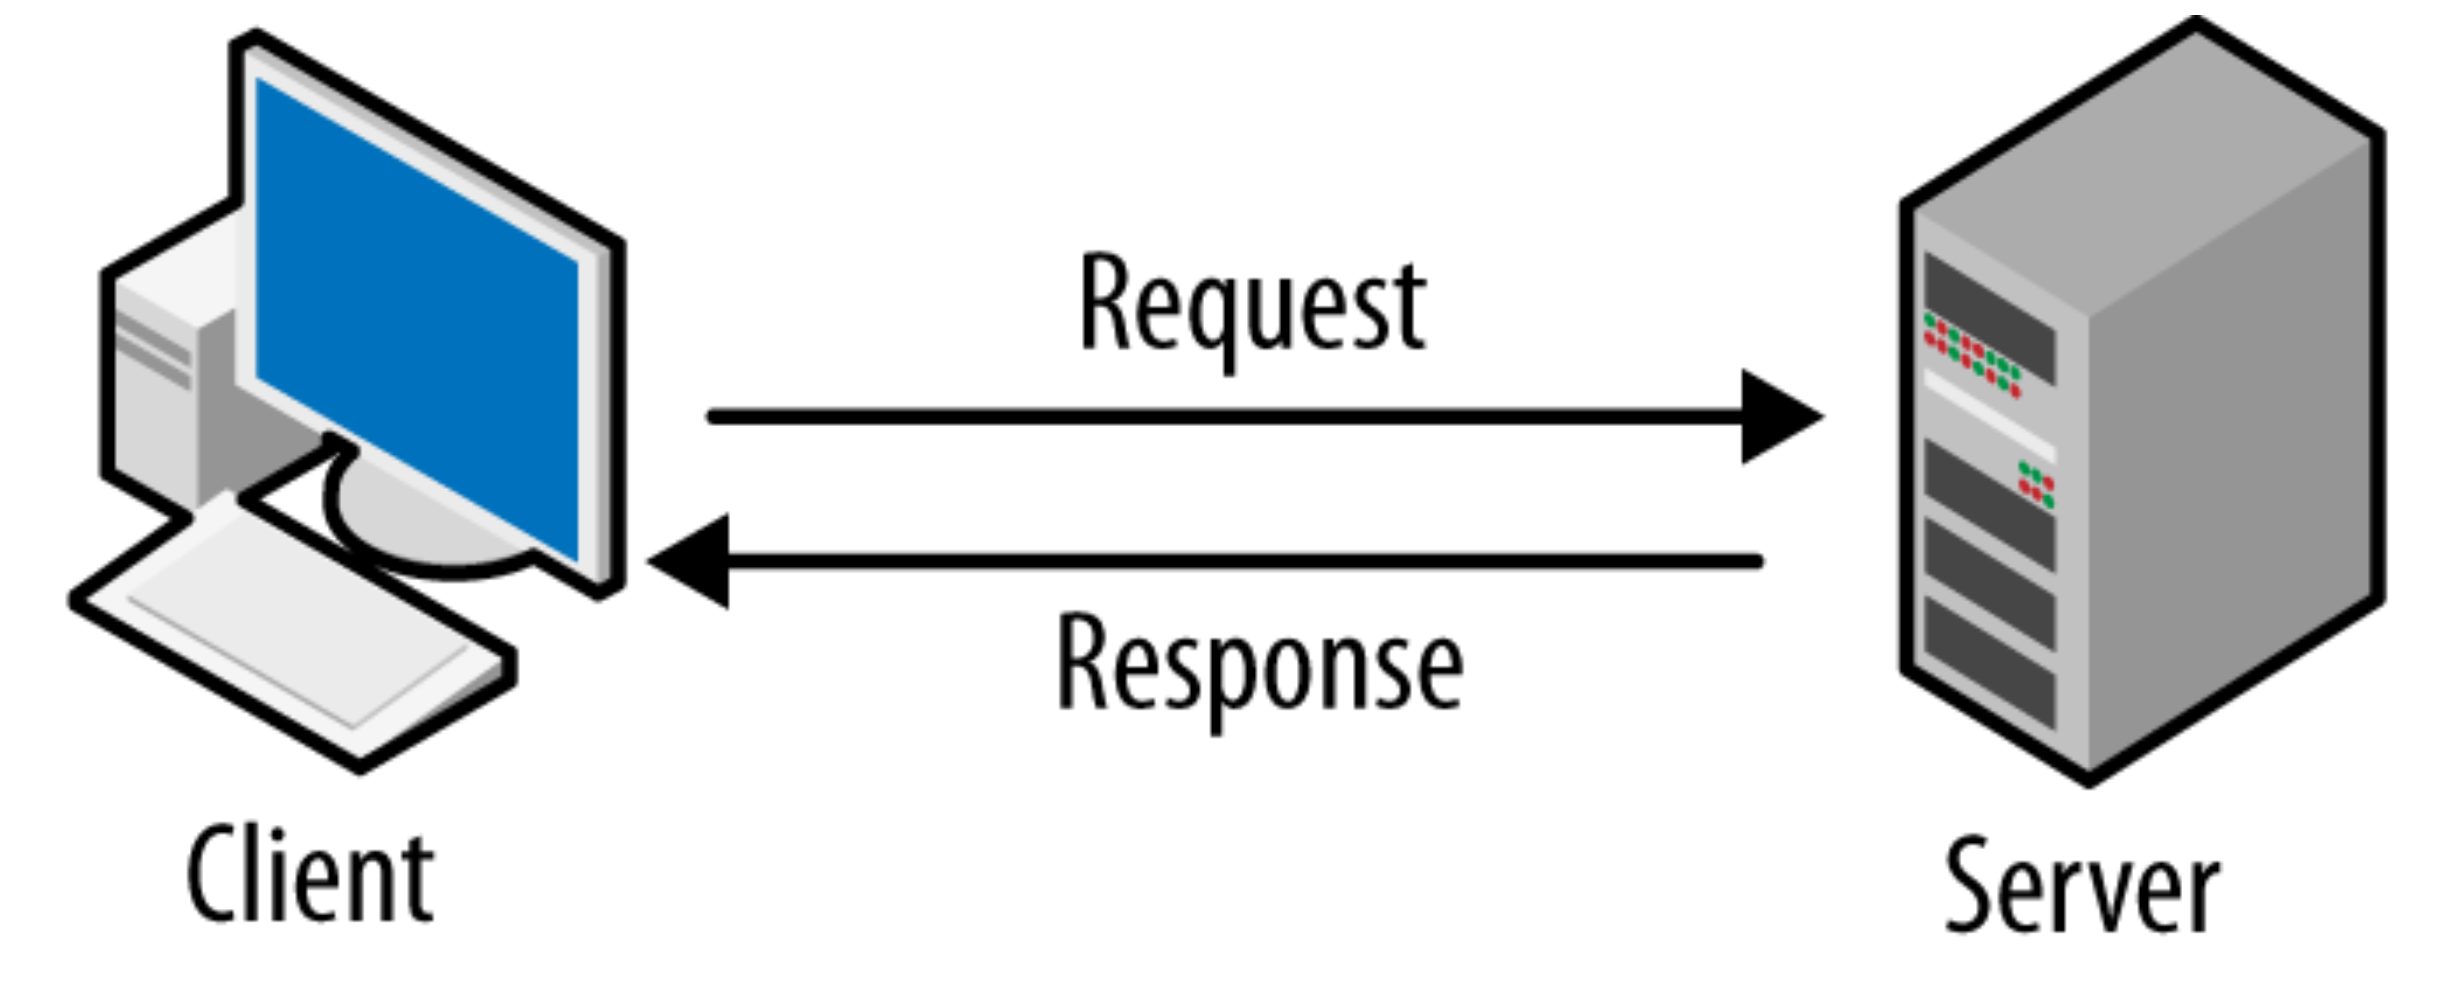
\includegraphics[width=100mm, scale=2]{figs/clientServerArch.png}
    \caption{Arhitectura 3-tier. Sursa~\cite{ClientServer}}
	\label{fig:clientServerArch}
\end{figure}
\ \\

Protocolul HTTP este un protocol request-reponse, care se bazează pe o arhitectură client-server. \\

Un {\it HTTP request} reprezintă modalitatea prin care browserul web, în cazul acestui proiect, solicită resurse. Fiecare request conține:
\begin{itemize}
	\setlength\itemsep{0.5em}
    \item Versiunea HTTP
    \item URL (Uniform Resource Locator)
    \begin{itemize}
		\setlength\itemsep{0.5em}
        \item Informații despre locația resursei solicitată de client
    \end{itemize}
    \item Metoda HTTP
    \begin{itemize}
		\setlength\itemsep{0.5em}
        \begingroup \color{blue}
        \item GET \endgroup
        \item HEAD
        \begingroup \color{blue}
        \item POST \endgroup
        \begingroup \color{blue}
        \item GET \endgroup
        \begingroup \color{blue}
        \item DELETE \endgroup
        \item TRACE
        \item OPTIONS
        \item CONNECT
        \item PATCH
    \end{itemize}
    \item HTTP Request Header
    \begin{itemize}
		\setlength\itemsep{0.5em}
        \item Conține informații despre browser-ul clientului, resursa cerută, encoding, server, etc.
    \end{itemize}
    \item Body (opțional, doar pentru anumite requesturi)
    \begin{itemize}
		\setlength\itemsep{0.5em}
        \item Conține informații transmise serverului (pentru anumite metode HTTP)
    \end{itemize}
\end{itemize}
\ \\

Un {\it HTTP response} este informația pe care o primesc clienții de la server ca răspuns la request. Acest răspuns conține:
\begin{itemize}
	\setlength\itemsep{0.5em}
    \item Status
    \begin{itemize}
		\setlength\itemsep{0.5em}
        \item Cod din 3 cifre care indică dacă requestul a fost încheiat cu succes
    \end{itemize}
    \item HTTP Response Header
    \begin{itemize}
		\setlength\itemsep{0.5em}
        \item Conține informații despre limba și formatul conținutului din body
    \end{itemize}
    \item Body
    \begin{itemize}
		\setlength\itemsep{0.5em}
        \item Conține informația solicitată printr-un request
    \end{itemize}
\end{itemize}
%%%%%%%%%%%%%%%%%%%%%%%%%%%%%%%%%%%%%%%%%%%%%%%%%%%%%%%%%%%%%%%%%%%%%%%%%%%%%%%%%%%%%%%%%%%%%%%%%%%%%%%%%%%%%%%%%%%%%%%%%%%%%%%%%%%%%%%%%%%%
\subsection{Arhitectura 3-Tier}
Arhitectura 3-Tier sau 3-Layer este o arhitectură pe 3 nivele: 
\begin{itemize}
	\setlength\itemsep{0.5em}
    \item Nivelul prezentării
    \begin{itemize}
        \setlength\itemsep{0.5em}
        \item Acest nivel este reprezentat de modulul de front-end al aplicație, interfața cu care utilizatorii vor interacționa în mod direct
        \item Acest nivel a fost construit în aplicație folosind:
        \begin{itemize}
            \setlength\itemsep{0.5em}
            \item Librăria {\it React Typescript}
            \item Pentru componente, este utilizată libraria {\it Ant Design}
            \item Pentru customizarea componentelor s-a utilizat {\it Styled Components}, un framework pentru stilizare, CSS-in-JS
        \end{itemize}
    \end{itemize}
    \item Nivelul aplicației
    \begin{itemize}
        \setlength\itemsep{0.5em}
        \item Acest nivel este reprezentat de modulul de back-end al aplicației
        \item Aici sunt procesate informațiile primite de la nivelul superior, cel de prezentare
        \item Nivelul interacționează în mod direct cu serverul. Acesta transmite cererea clientului la server, la fel și răspunsul serverului către client
        \item Pentru implementarea acestui nivel în aplicație, am folosit:
        \begin{itemize}
            \setlength\itemsep{0.5em}
            \item .NET Framework
            \item Entity Framework Core, un Object-Relational Mapper, care creează un layer între limbaj și baza de date
            \item MediatR, implementarea în .NET a patternului
        \end{itemize}
    \end{itemize}
    \item Nivelul datelor
    \begin{itemize}
        \setlength\itemsep{0.5em}
        \item Cunoscut ca nivelul bazei de date
        \item Aici se găsesc servere de baze de date unde se pot stoca și prelua informații
        \item Pentru acest nivel, am folosit Microsoft SQL Server
    \end{itemize}
\end{itemize}
\vspace{1em}
Avantajul utilizării acestui pattern arhitectural este că permite ca un layer să fie modificat, fără să fie afectate celelalte.
\begin{figure}[h]
	\centering
	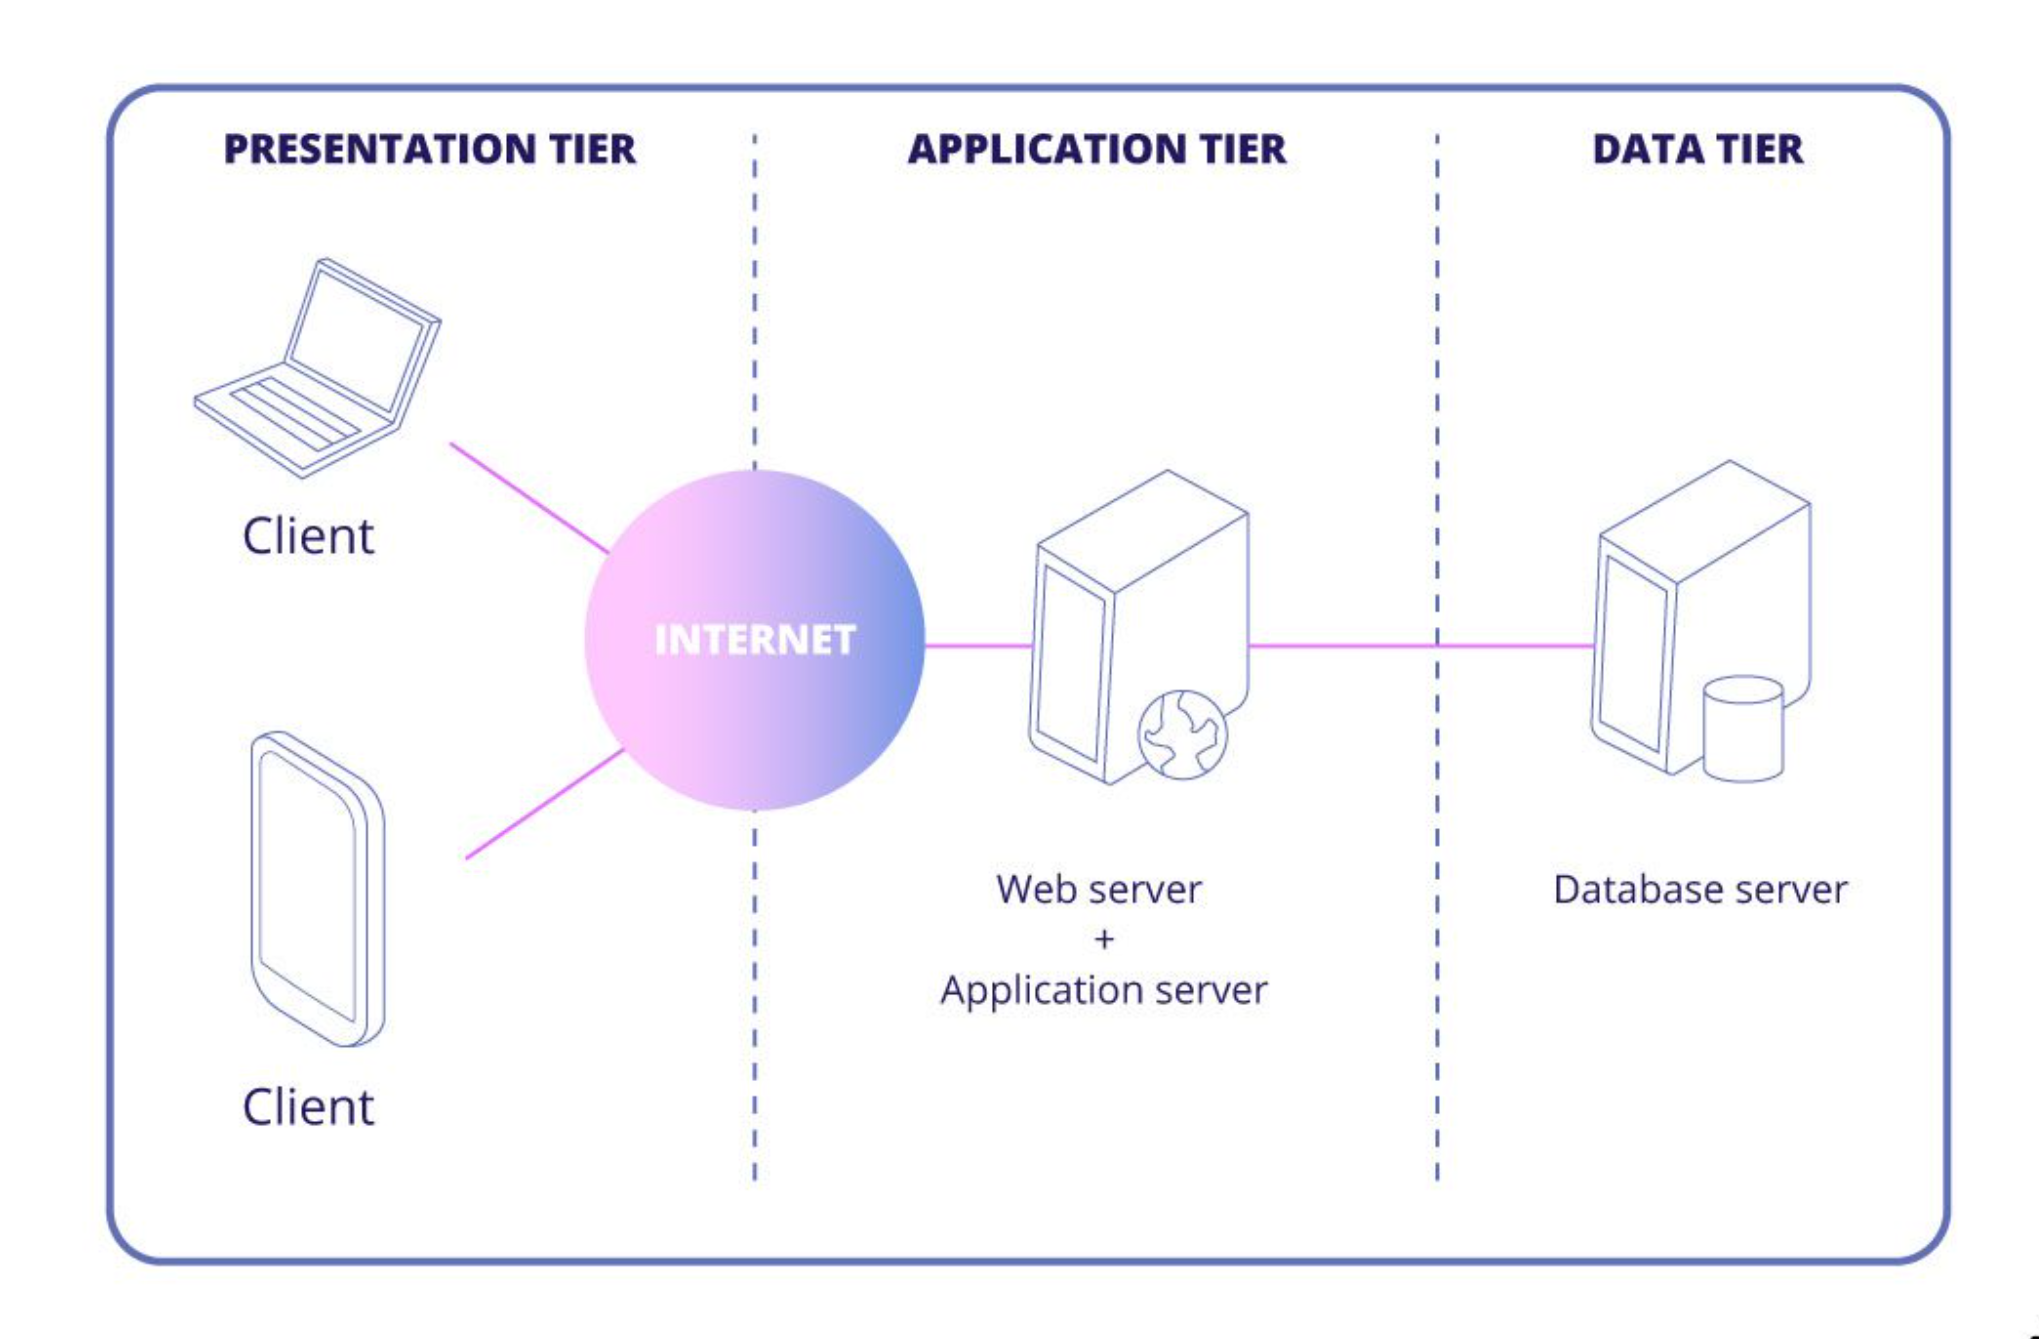
\includegraphics[width=100mm, scale=1]{figs/threetier.png}
    \caption{Arhitectura 3-tier. Sursa~\cite{ThreeTier}}
	\label{fig:threetier}
\end{figure}
%%%%%%%%%%%%%%%%%%%%%%%%%%%%%%%%%%%%%%%%%%%%%%%%%%%%%%%%%%%%%%%%%%%%%%%%%%%%%%%%%%%%%%%%%%%%%%%%%%%%%%%%%%%%%%%%%%%%%%%%%%%%%%%%%%%%%%%%%%%%
\subsection{Mediator Design Pattern}
Scopul utilizării acestui design pattern este de a reduce dependințele dintre obiecte, restricționând comunicarea între obiecte și mijlocind colaborarea printr-un mediator. \\

\noindent Avantajele utilizării mediatorului sunt:
\begin{itemize}
	\setlength\itemsep{0.5em}
    \item Comunicarea între mai multe componente poate fi extrasă într-un singur loc, fiind mai ușor de înțeles și modificat, acolo unde e cazul (Single Responsability Principle)
    \item Se pot introduce noi mediatori fără a schimba componentele deja existente
    \item Cuplarea între componente este redusă {\it (Low coupling)}
\end{itemize}
\begin{figure}[H]
	\centering
	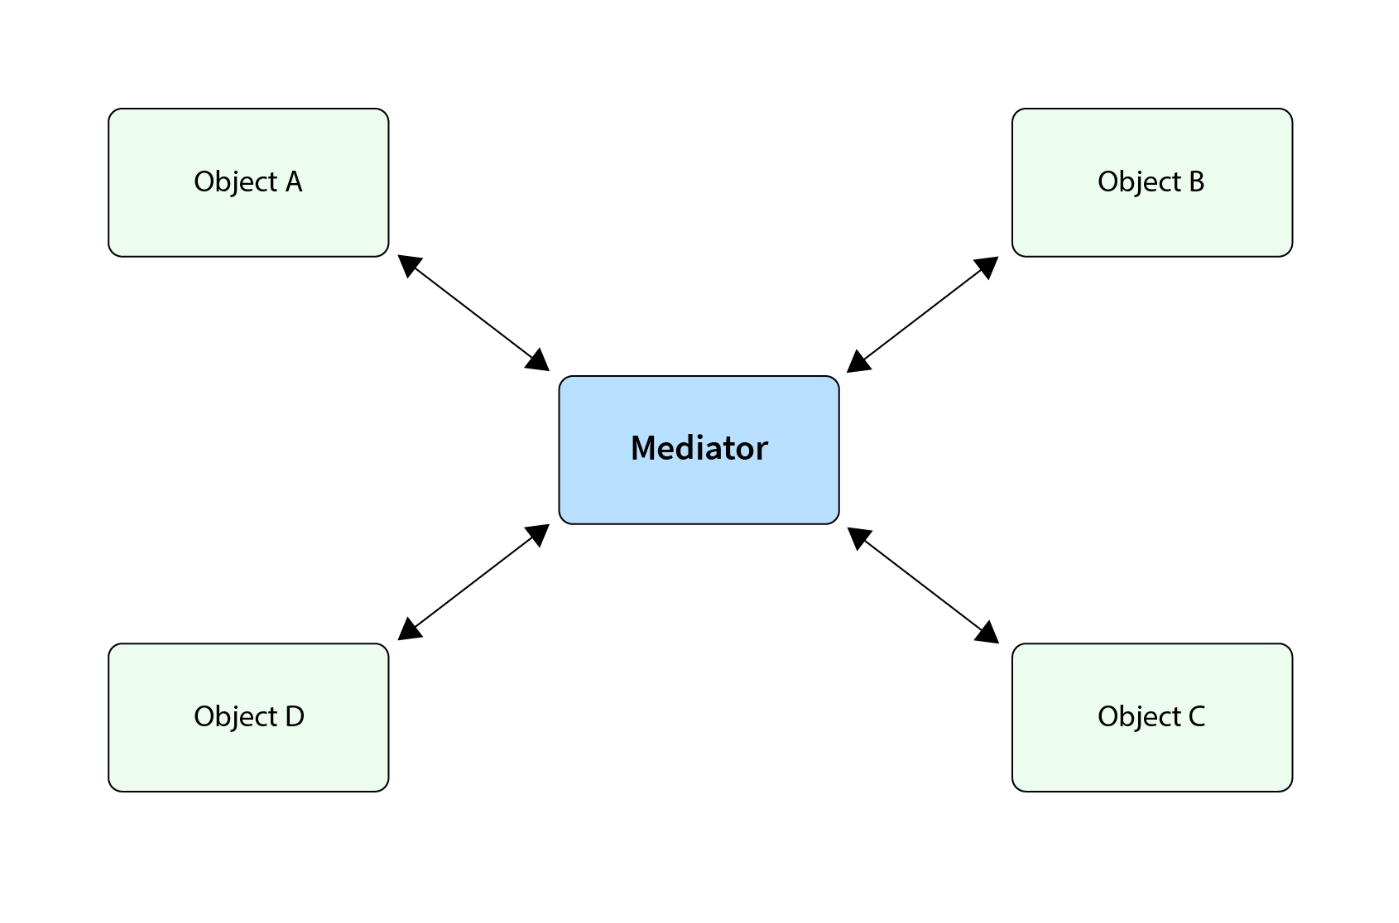
\includegraphics[width=100mm, scale=1]{figs/mediator.png}
    \caption{Diagramă Mediator Design Pattern. Sursa~\cite{Mediator}}
	\label{fig:mediator}
\end{figure}
%%%%%%%%%%%%%%%%%%%%%%%%%%%%%%%%%%%%%%%%%%%%%%%%%%%%%%%%%%%%%%%%%%%%%%%%%%%%%%%%%%%%%%%%%%%%%%%%%%%%%%%%%%%%%%%%%%%%%%%%%%%%%%%%%%%%%%%%%%%%
\subsection{CQRS}
Command-Query Responsibility Segregation sau CQRS este un design pattern care separă comenzile de interogări.\\
Comenzile sunt cele care scriu sau actualizează date în baza de date, iar o interogare citește datele din baza de date.
 
\begin{figure}[H]
	\centering
	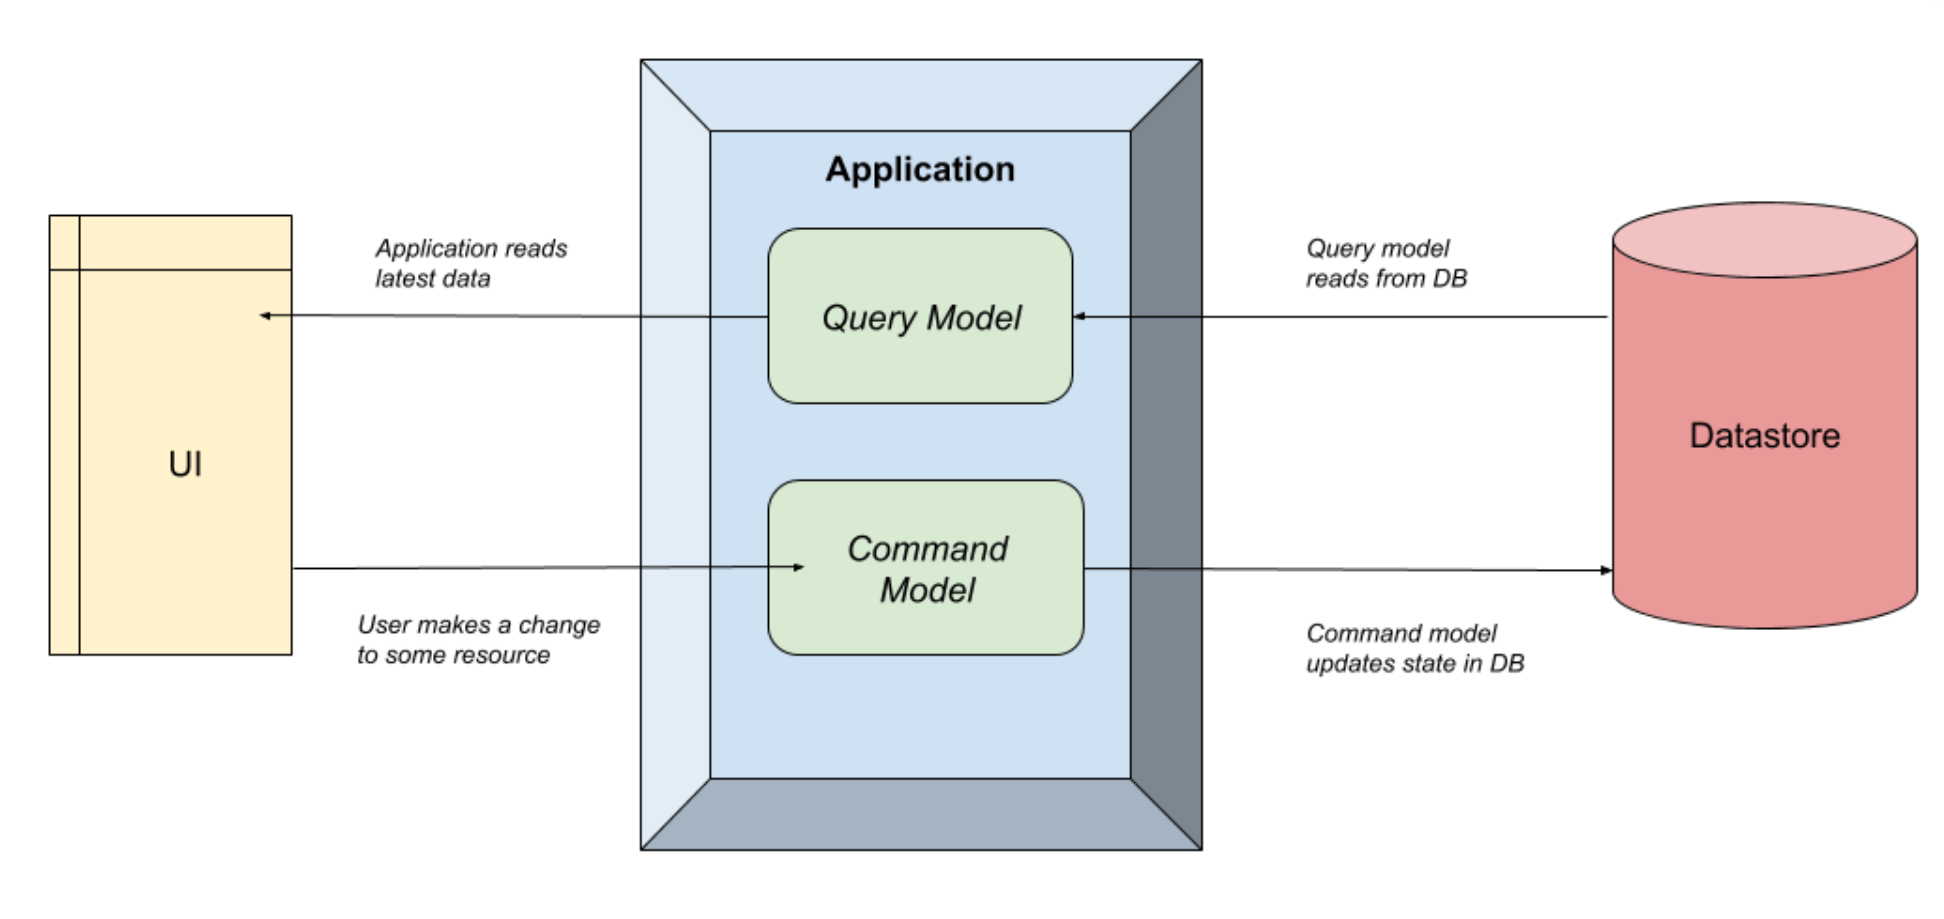
\includegraphics[width=100mm, scale=2]{figs/cqrs.png}
    \caption{Diagramă CQRS. Sursa~\cite{CQRS}}
	\label{fig:cqrs}
\end{figure}
%%%%%%%%%%%%%%%%%%%%%%%%%%%%%%%%%%%%%%%%%%%%%%%%%%%%%%%%%%%%%%%%%%%%%%%%%%%%%%%%%%%%%%%%%%%%%%%%%%%%%%%%%%%%%%%%%%%%%%%%%%%%%%%%%%%%%%%%%%%%
\subsection{Fluent Validation}
Fluent Validation este o librarie  din .NET pentru validarea modelelor. \\ 
Avantajul folosirii acestei librarii constă în faptul că logica de validare poate fi separată de modele și se renunță la adnotări.

În exemplul din figura \ref{fig:fluentValidation}, câmpul de firstName a fost completat cu un string gol, deși în validator modelul trebuie să aibă acest câmp este marcat ca fiind {\it required}.
De asemenea, a fost adăugată o validare extra pentru numărul de caractere și, fiind încălcată, este menționată în răspunsul din Swagger.
\begin{figure}[H]
	\centering
	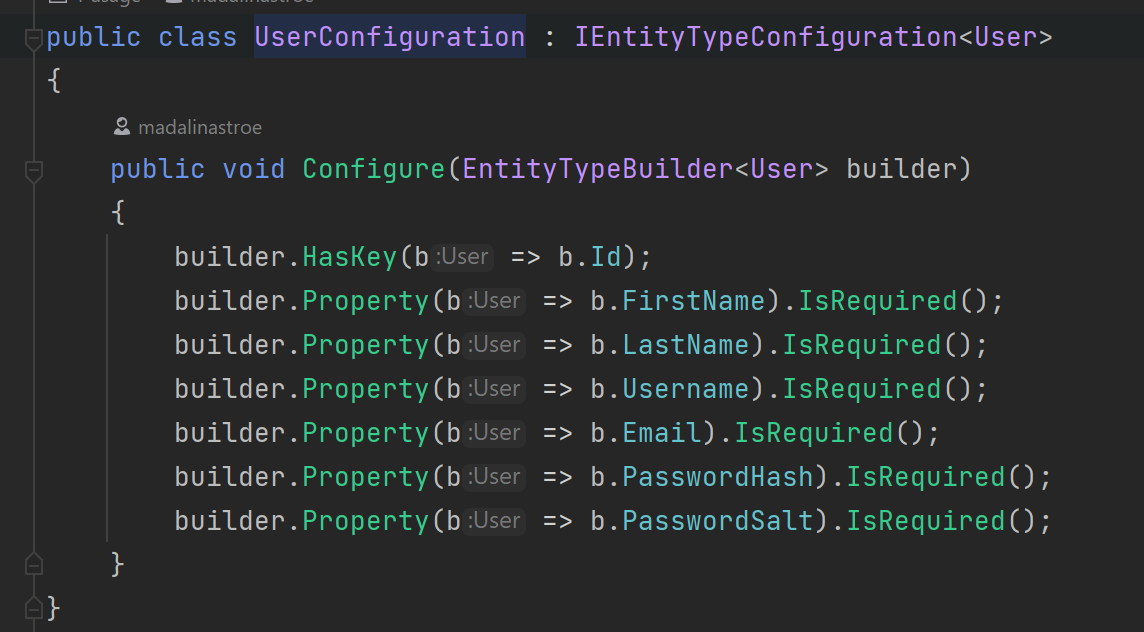
\includegraphics[width=100mm, scale=2]{figs/userConfigValidation.png}
	\caption{Configurare validări pentru modelul unui utilizator}
	\label{fig:userConfigValidation}
\end{figure}

\begin{figure}[H]
	\centering
	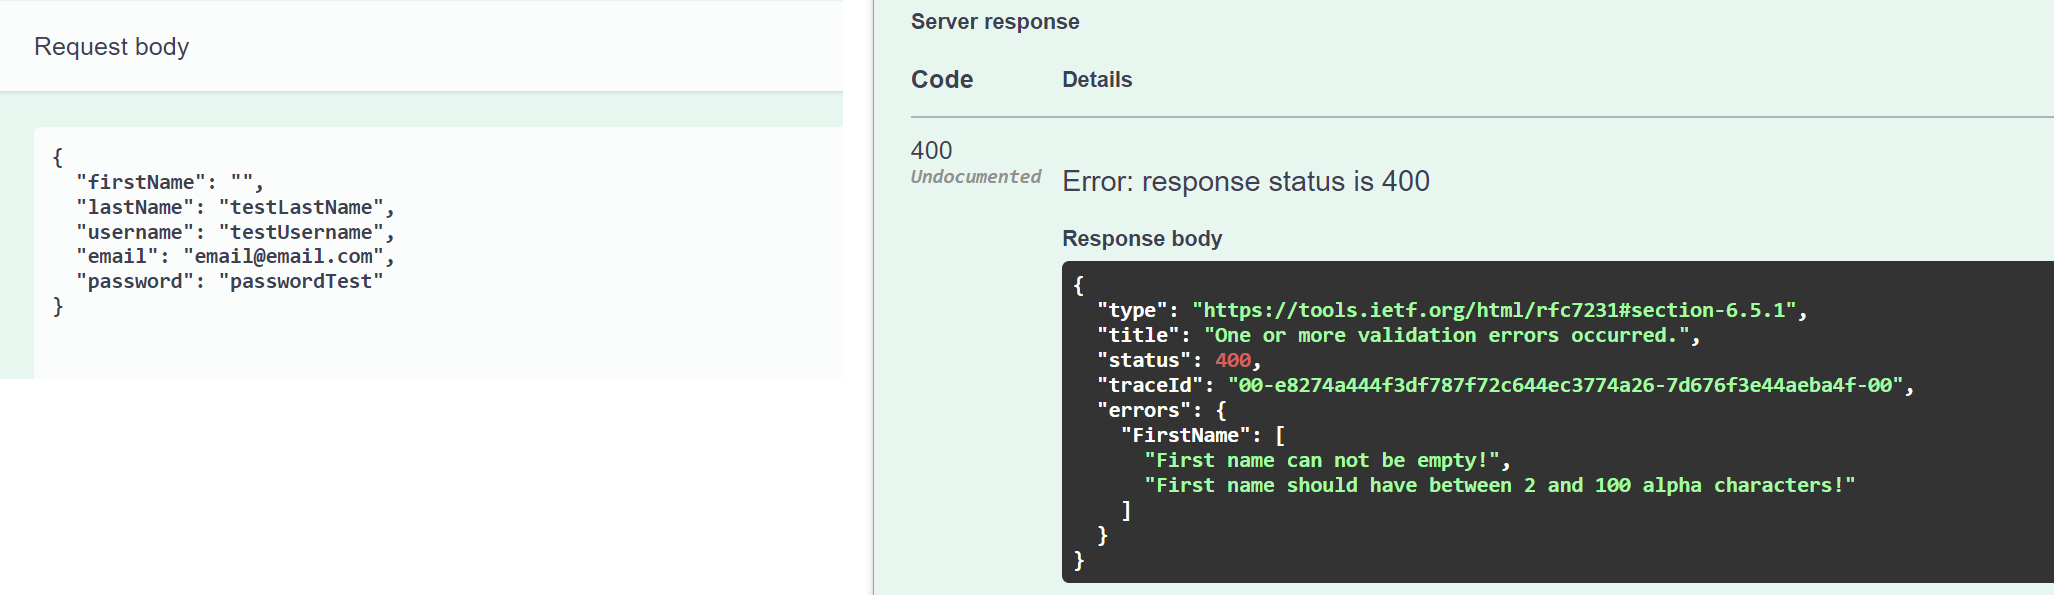
\includegraphics[width=150mm]{figs/fluentValidations.png}
	\caption{Request - Response folosind Fluent Validation}
	\label{fig:fluentValidation}
\end{figure}
%%%%%%%%%%%%%%%%%%%%%%%%%%%%%%%%%%%%%%%%%%%%%%%%%%%%%%%%%%%%%%%%%%%%%%%%%%%%%%%%%%%%%%%%%%%%%%%%%%%%%%%%%%%%%%%%%%%%%%%%%%%%%%%%%%%%%%%%%%%%
\section{Modul frontend}
\subsection{React}
Este un framework pentru dezvoltarea interfeței utilizator. Cu ajutorul acesteia, codul scris și componentele devin reutilizabile.\\
A fost dezvoltat de Facebook în 2011 și este cel mai popular framework din acest moment. 
Avantajele folosirii React sunt: 
\begin{itemize}
	\setlength\itemsep{0.5em}
    \item Ușor de învățat și folosit
    \item Componentele sunt reutilizabile
    \item Oferă flexibilitate
    \item SEO friendly
\end{itemize}

\begin{figure}[H]
	\centering
	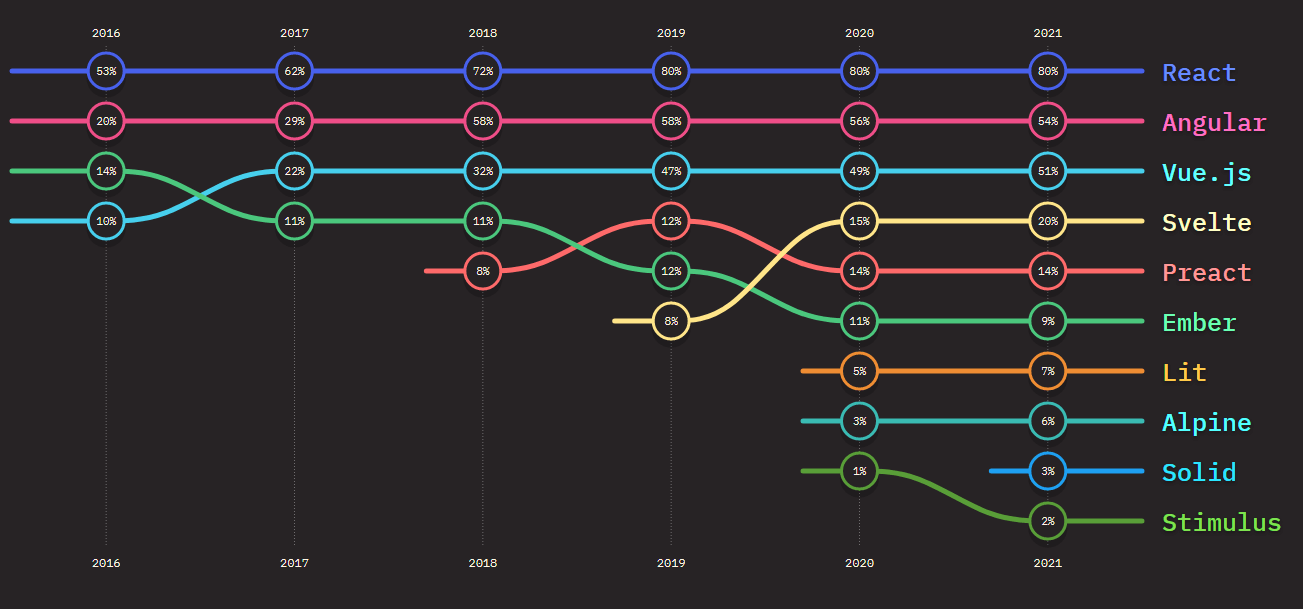
\includegraphics[width=100mm, scale=2]{figs/uiFrameworks.png}
    \caption{Cele mai populare frameworkuri pentru UI. Sursa~\cite{UIPopularity}}
    \label{fig:uiFrameworks}
\end{figure}
%%%%%%%%%%%%%%%%%%%%%%%%%%%%%%%%%%%%%%%%%%%%%%%%%%%%%%%%%%%%%%%%%%%%%%%%%%%%%%%%%%%%%%%%%%%%%%%%%%%%%%%%%%%%%%%%%%%%%%%%%%%%%%%%%%%%%%%%%%%%
\subsection{Ant Design}
Este o librărie din React, care conține componente ușor de utilizat.
Componentele pot fi customizate cu ajutorul designului oferit de librarie, dar și din exterior, cu ajutorul CSS.
Avantajele folosirii acestei librării sunt: 
\begin{itemize}
	\setlength\itemsep{0.5em}
    \item Design-ul consistent și accesibil
    \item Suport pentru Typescript și Javascript
    \item Form-uri ușor de customizat
    \item Variații pentru fiecare component
\end{itemize}
%%%%%%%%%%%%%%%%%%%%%%%%%%%%%%%%%%%%%%%%%%%%%%%%%%%%%%%%%%%%%%%%%%%%%%%%%%%%%%%%%%%%%%%%%%%%%%%%%%%%%%%%%%%%%%%%%%%%%%%%%%%%%%%%%%%%%%%%%%%%
\subsection{Styled Components}
Folosind CSS-in-JS, cu ajutorul librarie styled-components, componentele pot fi ajustate aplicând direct un stil customizat.
Avantajele folosirii sunt:
\begin{itemize}
	\setlength\itemsep{0.5em}
    \item Reutilizarea - precum componentele din React, pentru a evita duplicarea, acesta poate fi reutilizabil atunci când se aplică pe componente
    \item CSS
    \item Generează nume unice pentru fiecare clasa pentru targetarea corectă a componentelor
\end{itemize}

\begin{figure}[ht]
	\centering
	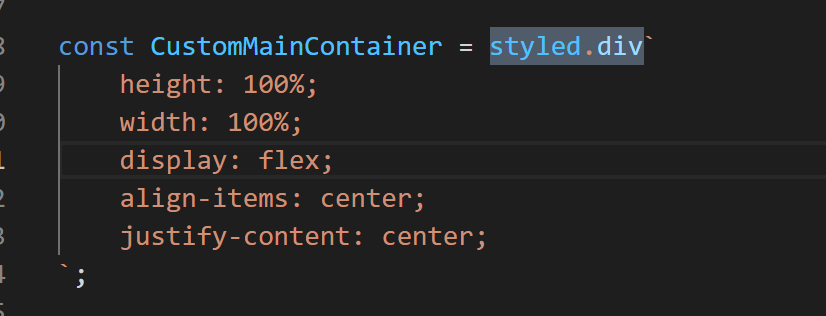
\includegraphics[width=100mm, scale=2]{figs/styledcomp.png}
	\caption{Exemplu utilizare styled-components}
	\label{fig:styledcomp}
\end{figure}
%%%%%%%%%%%%%%%%%%%%%%%%%%%%%%%%%%%%%%%%%%%%%%%%%%%%%%%%%%%%%%%%%%%%%%%%%%%%%%%%%%%%%%%%%%%%%%%%%%%%%%%%%%%%%%%%%%%%%%%%%%%%%%%%%%%%%%%%%%%%
\subsection{i18n}
Librăria i18next este folosită pentru internaționalizarea proiectului; mai exact, cu ajutorul acesteia rezolvăm partea de traducere a aplicației.\\
În acest fel, foarte simplu, tot conținutul aplicației poate fi schimbat în limba dorită, dacă sunt adăugate traducerile corespunzătoare.
%%%%%%%%%%%%%%%%%%%%%%%%%%%%%%%%%%%%%%%%%%%%%%%%%%%%%%%%%%%%%%%%%%%%%%%%%%%%%%%%%%%%%%%%%%%%%%%%%%%%%%%%%%%%%%%%%%%%%%%%%%%%%%%%%%%%%%%%%%%%
\section{Modele de Procesare a limbajului natural}
\subsection{FinBERT}
Bidirectional Encoder Representations from Transformers sau BERT este unul dintre cele mai folosite modele în Procesarea de Limbaj Natural din ultimii ani.
Este diferit față de modelele din anii anteriori, având un mecanism de self-attention, procesând textul bidirecțional.\\

Ce reprezintă un mecanism {\it self-attention}? În secțiunea "Self-Attention at a High Level" din~\cite{IllustratedTransformer},
rezumând câteva idei principale din publicația Attention Is All You Need~\cite{TransformerModel}, self-attention este o metodă folosită pentru a "privi" alte cuvinte relevante din enunț în timpul procesării cuvântului curent.
Bert~\cite{BERT} se bazează pe arhitectura Transformer~\cite{TransformerModel}, un model care a apărut în 2017, care depinde de aproximativ o sută de milioane de parametri.\\

\noindent Arhitectura Transformer, în figura \ref{fig:transformersArch}, este compusă din următoarele părți: 
\begin{itemize}
    \setlength\itemsep{0.5em}
    \item Tokenizarea textului
    \item Codificarea poziționala care injectează informații despre poziția inputului
    \item Codificarea contextuală a secvenței de intrare, pe nivelul de self-attention
    \item Nivelul feed forward care funcționează ca o memorie statică, cheie-valoare
    \item Nivelul de cross-atention decodifică secvența de ieșire
\end{itemize}
\begin{figure}[ht]
	\centering
	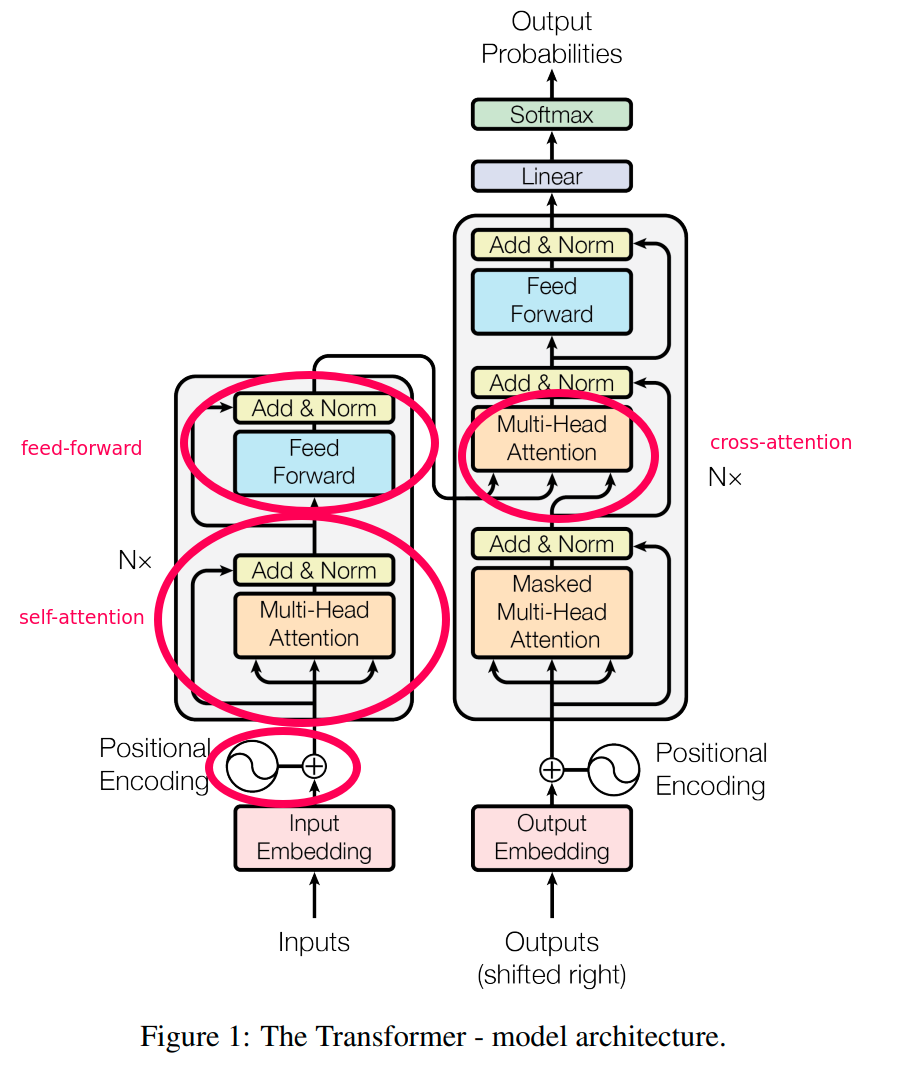
\includegraphics[width=100mm, scale=0.5]{figs/transformersArch.png}
    \caption{Arhitectura Transformers. Sursa~\cite{Transformers}}
	\label{fig:transformersArch}
\end{figure}
\ \\
În BERT, inputul este adus în primul nivel, apoi este transformat în alte codificări în următoarele nivele. 
Spre deosebire de abordările dinainte, prima etapă este etapa de pre-antrenare (en: pre-training), unde folosește 2 task-uri nesupervizate.
După această etapă, modelul poate să fie perfecționat pentru o sarcină specifică, precum analiza de sentimente. \\

Analiza de sentimente pentru un text reprezintă extragerea sentimentelor sau opiniilor oamenilor dintr-un text scris.
Analiza sentimentelor financiare diferă de analiza de sentimente prin scopul ei, pentru că rezultatul acestei analize va determina modul în care piața va fi influențată de deciziile financiare.\\
În~\cite{FinBERT1}, autorii spun despre FinBERT că este un model de analiză a textului bazat pe BERT, cu un domeniu specific. Acest model a fost antrenat pe un corpus de 4.9 miliarde de tokeni compuși din rapoarte ale companiilor, transcripturi ale conferințelor și rapoarte de analiză, conform \cite{FinBERT2}.\\

În Statele Unite ale Americii, toate companiile cotate la bursă depun rapoarte anuale, cunoscute sub numele de Form 10-K și rapoarte trimestriale, cunoscute sub numele de 10-Q. Aceste documente sunt publice și oferă o imagine de ansamblu a situației financiare a companiei.\\
Cele menționate mai sus, alături de rapoarte ale analiștilor, care oferă măsuri rezumative cu recomandări, și teleconferințe trimestriale pe care directorii companiilor le au cu investitorii pentru a discuta despre performanța firmei, formează un corpus financiar. \\
Un corpus sau corpora reprezintă o colecție de texte sau fișiere audio organizate în seturi de date (en: datasets). Un corpus este, în general, folosit pentru antrenarea sistemelor bazate pe Inteligență Artificială. 
%%%%%%%%%%%%%%%%%%%%%%%%%%%%%%%%%%%%%%%%%%%%%%%%%%%%%%%%%%%%%%%%%%%%%%%%%%%%%%%%%%%%%%%%%%%%%%%%%%%%%%%%%%%%%%%%%%%%%%%%%%%%%%%%%%%%%%%%%%%%
\subsection{Sumarizator de text}
Sumarizarea este procesul de producere a unei versiuni mai scurte a unui text sau document, păstrând ideile importante din textul original.
Deși modelul BERT este folosit pentru multe task-uri de NLP, în diferite domenii și subdomenii, acesta nu este soluția și pentru sumarizarea textului sau traduceri. În acest caz, apare BART (Denoising Sequence-to-Sequence Pre-training for Natural
Language Generation, Translation, and Comprehension), care folosește arhitectura sequence-to-sequence din Transformers și este un model folosit pentru clasificarea și generarea textului.\\
Este implementat ca un model sequence-to-sequence cu un codificator bidirecțional pentru textul corupt și un decodificator stânga-dreapa.
Arhitectura este asemănătoare cu arhitectura BERT, cu câteva diferențe, menționate în ~\cite{BARTArchitecture}: 
\begin{itemize}
    \setlength\itemsep{0.5em}
    \item Fiecare nivel al decodificatorului efectuează suplimentar funcția de cross-atention pe ultimul strat ascuns al codificatorului
    \item BERT folosește o rețea feed-forward suplimentară, spre deosebire de BART
\end{itemize}
\ \\
Acest model este pre-antrenat folosind un framework {\it Corrupt and Reconstruct}~\cite{CorruptAndReconstruct} care ia un text, aplică o funcție de zgomot, apoi antrenează modelul să reconstruiască textul original. 
Printre funcțiile de zgomot avem: 
\begin{itemize}
    \setlength\itemsep{0.5em}
    \item Mascarea tokenilor (Token Masking) - se maschează anumiți token și se încearcă reconstrucția textului original
    \item Ștergerea tokenilor (Token deletion) - se șterg anumiți token și se încearcă reconstrucția textului original
    \item Rotația documentului (Document Rotation) - Mutarea anumitor tokeni pentru ca modelul să identifice începutul secvenței
    \item Permutarea enunțului (Sentence Permutation) - Se iau toate frazele din document și sunt amestecate
    \item Completarea texului (Text infilling) - Un număr fix de tokeni este șters și înlocuit cu o singură mască. Modelul învață să prezică numărul de tokeni ce lipsesc dintr-un span și conținutul acestora~\cite{SpanBERT}
\end{itemize}
\begin{figure}[H]
	\centering
	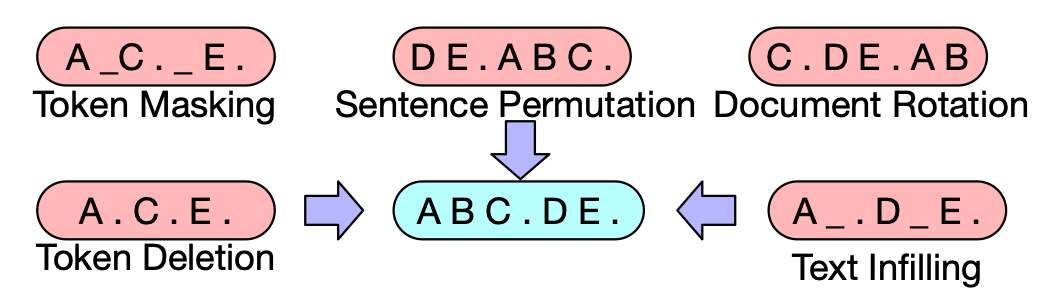
\includegraphics[width=100mm, scale=0.5]{figs/bartNoise.png}
    \caption{BART - Funcții de zgomot (Noising Functions). Sursa~\cite{BART}}
	\label{fig:bartNoise}
\end{figure}

BART este folosit pentru sumarizarea textului; în funcție de abordare, aceasta poate fi de două tipuri: abstractivă sau extractivă. \\
Sumarizarea extractivă identifică și extrage cele mai semnificative enunțuri din text, pe când, prin sumarizarea abstractivă,
se încearcă înțelegerea întregului text și generarea unui sumar cu un text parafrazat, cea de-a doua metodă fiind utilizată și de BART.
Modelul ales în acest proiect este bazat pe modelele DistilBART și este evaluat folosind metrica ROUGE~\cite{Rouge}, bazat pe suprapunerea dintre secvența produsă și secvența corectă. 
%%%%%%%%%%%%%%%%%%%%%%%%%%%%%%%%%%%%%%%%%%%%%%%%%%%%%%%%%%%%%%%%%%%%%%%%%%%%%%%%%%%%%%%%%%%%%%%%%%%%%%%%%%%%%%%%%%%%%%%%%%%%%%%%%%%%%%%%%%%%
\subsection{Keyphrase Extractor}
Extragerea de cuvinte sau fraze cheie reprezintă o tehnică prin care sunt extrase cuvintele părțile importante dintr-un text. \\
În~\cite{KBIR}, autorii spun că frazele sau cuvintele cheie captează cele mai importante idei și identificarea lor automată ajută foarte mult în sarcini precum clasificarea, sumarizarea, etc.
Modelul KBIR folosește o combinație de mascare a tokenilor (Masked Language Modeling - MLM), mascare a expresiilor (Keyphrase Bounday Infilling - KBI) și învățarea constrativă (Keyphrase Replacement Classification - KRC).

%%%%%%%%%%%%%%%%%%%%%%%%%%%%%%%%%%%%%%%%%%%%%%%%%%%%%%%%%%%%%%%%%%%%%%%%%%%%%%%%%%%%%%%%%%%%%%%%%%%%%%%%%%%%%%%%%%%%%%%%%%%%%%%%%%%%%%%%%%%%
\section{Aplicații similare}
În momentul de față, există destul de puține aplicații publice pentru analiza textelor financiare. 
\subsection{Serviciul de înțelegere a limbajului natural dezvoltat de IBM}
{\noindent Acest serviciu are următoarele funcționalități:}
\begin{itemize}
    \setlength\itemsep{0.5em}
    \item Analiza textului în mai multe domenii - Legal, Media și Financiar
    \item Textul analizat poate să fie copiat în field-ul din aplicație sau poate să fie referit prin URL
    \item Pentru partea de extracție din text, pot fi ca rezultat următoarele:
    \begin{itemize}
        \setlength\itemsep{0.5em}
        \item Entitațile extrase care pot aparține unui tip (ex: Organization, Job title, etc.)
        \item Cuvintele cheie extrase
        \item Conceptele extrase
        \item Relațiile dintre entitați
    \end{itemize}
    \item Pentru partea de clasificare a textului, pot fi ca rezultat următoarele:
    \begin{itemize}
        \setlength\itemsep{0.5em}
        \item Scorul sentimentului pe întregul document
        \item Scorul sentimentului pe fiecare entitate extrasă 
        \item Scorul sentimentului pe fiecare entitate cuvânt cheie sau frază 
        \item Clasificarea emoțiilor pe întregul document (ex: Sadness, Joy, Disgust, Fear, Anger, etc.)
        \item Clasificarea emoțiilor pentru fiecare entitate
        \item Clasificarea emoțiilor pentru fiecare cuvânt cheie sau frază
        \item Clasificarea în categorii, ierarhic
    \end{itemize}
    \item Pentru partea lingvistică a textului, pot fi ca rezultat următoarele:
    \begin{itemize}
        \setlength\itemsep{0.5em}
        \item Rolurile semantice (Subiect + Acțiune + Forma obiectului)
        \item Sintaxa - pentru fiecare token se specifică partea de vorbire
    \end{itemize}
\end{itemize}
\begin{figure}[H]
	\centering
	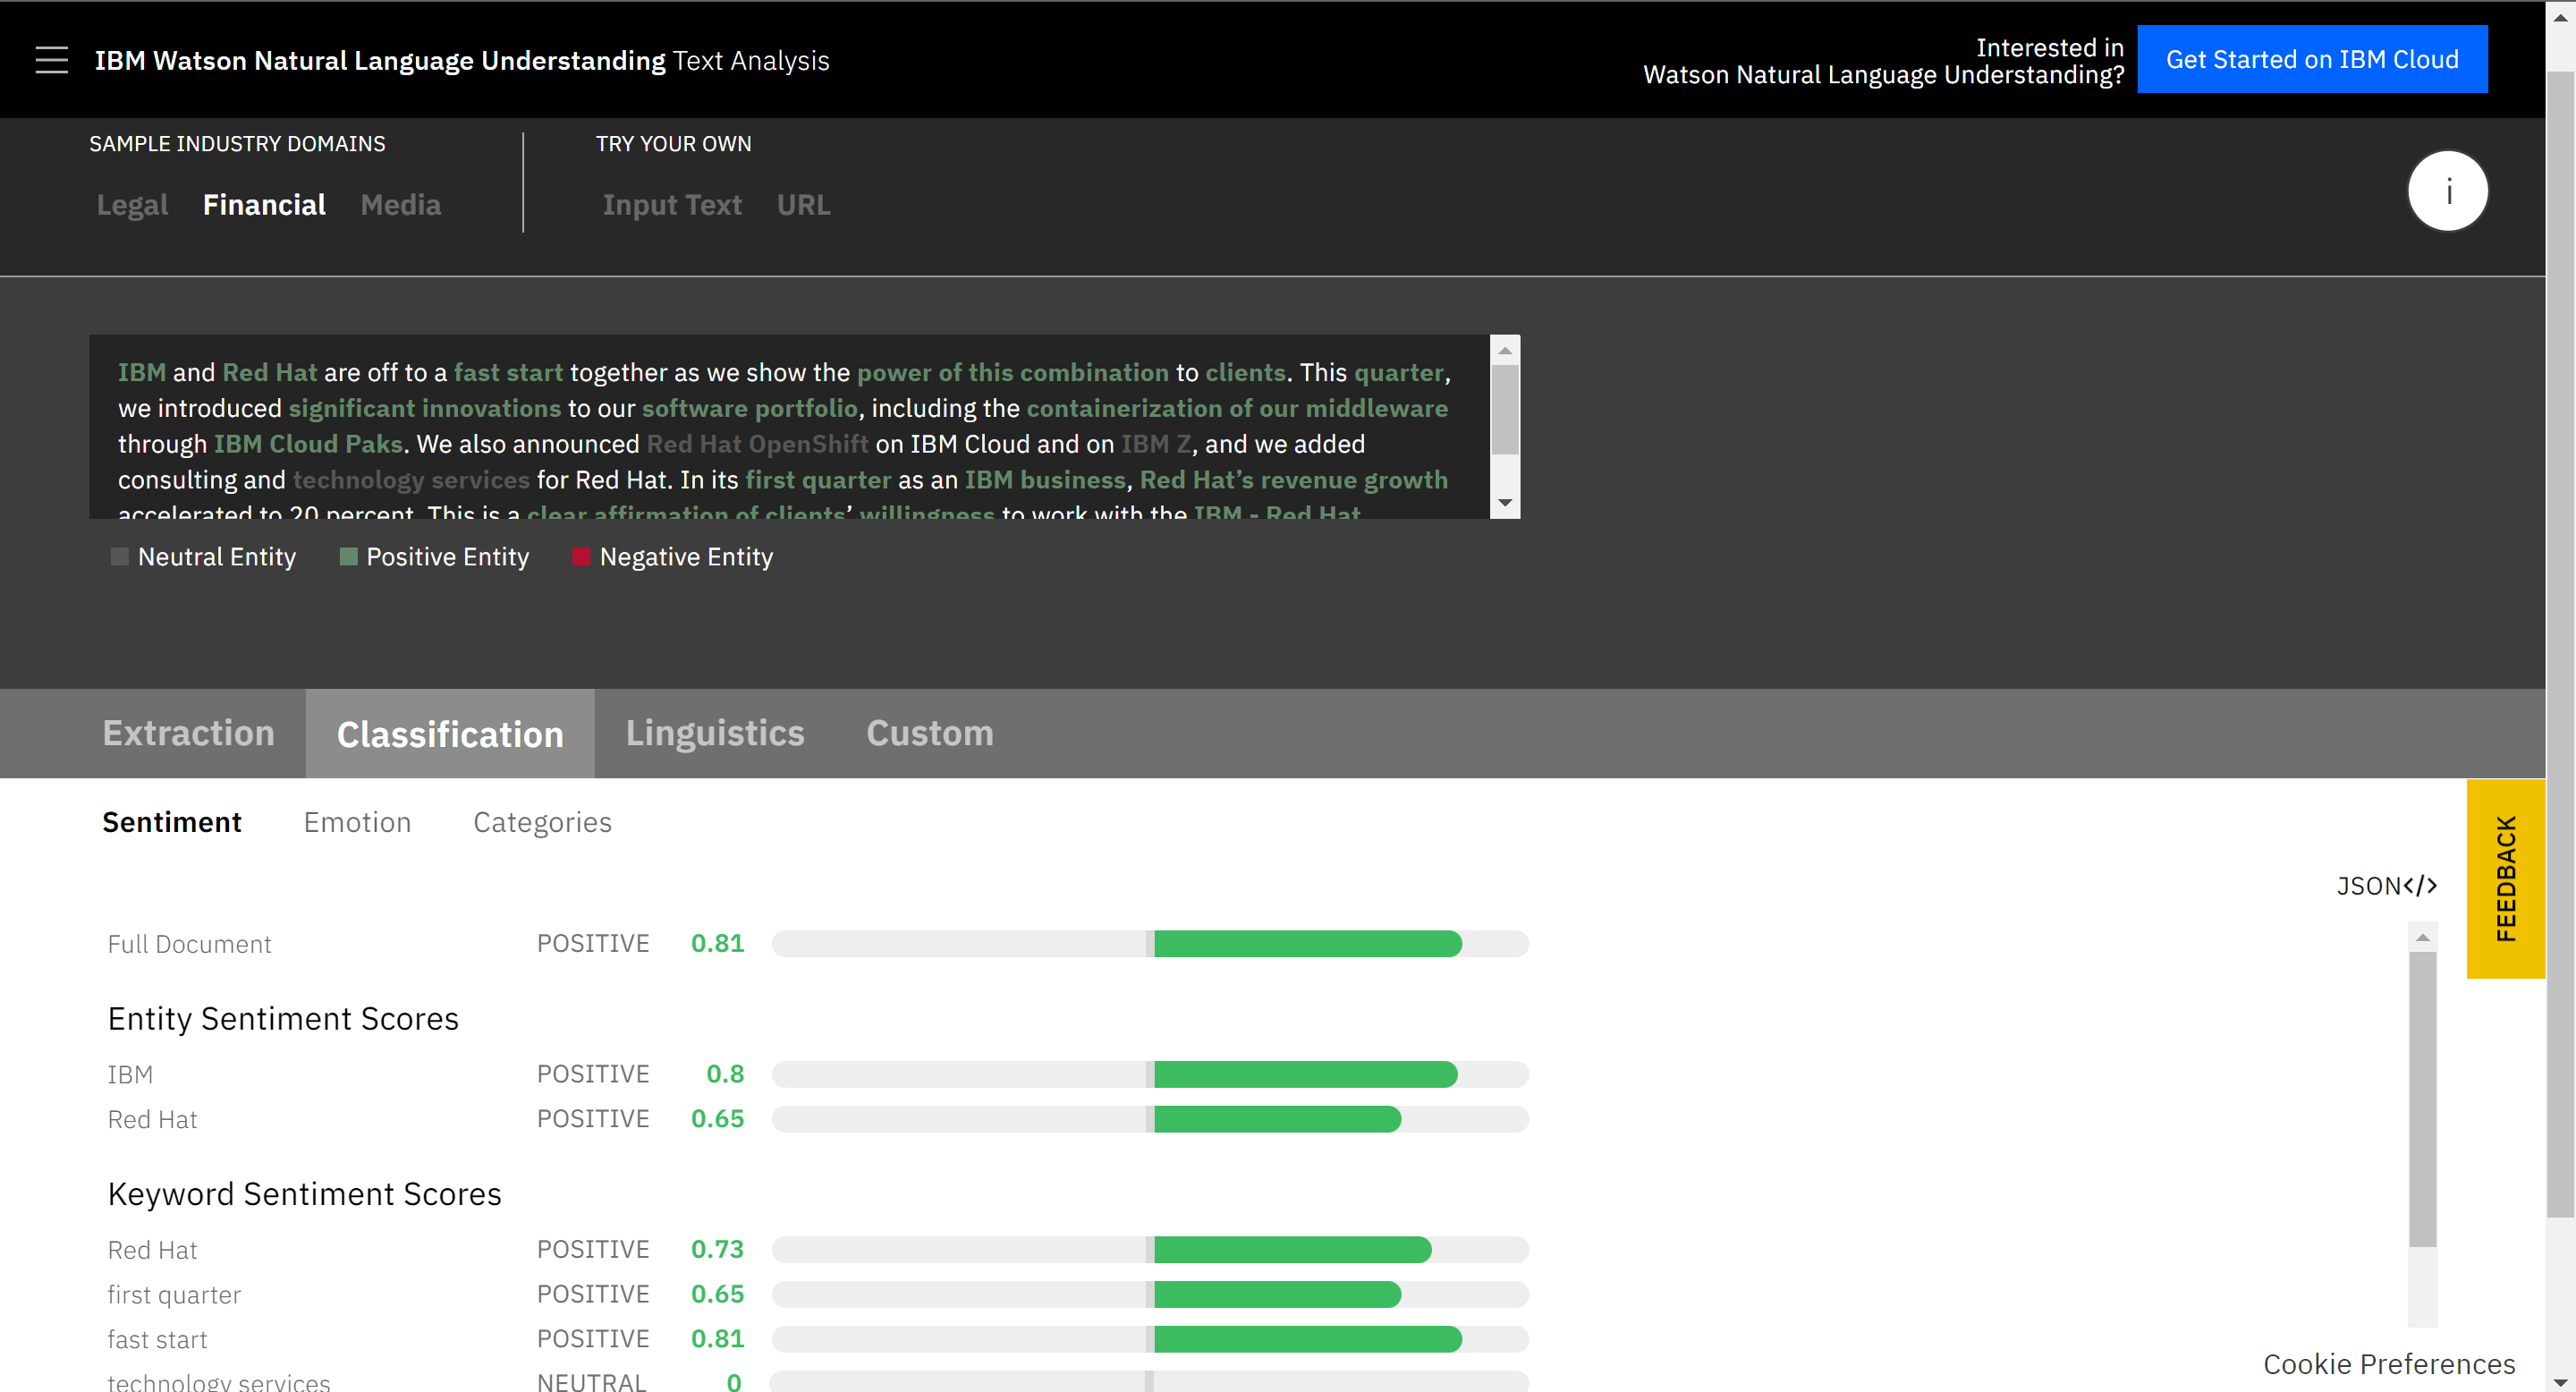
\includegraphics[width=150mm]{figs/ibmCloud.png}
    \caption{Servicii IBM}
	\label{fig:ibmCloud}
\end{figure}
\subsection{Google Cloud Natural Language}
{\noindent Acest serviciu are următoarele funcționalități:}
\begin{itemize}
    \setlength\itemsep{0.5em}
    \item Entitațile extrase care pot aparține unui tip (ex: Organization, Location, Person, Event, Other, etc.)
    \item Scorul sentimentului și magnitudinea pe întregul document
    \item Scorul sentimentului și magnitudinea pe fiecare entitate extrasă 
    \item Sintaxa - pentru fiecare token (inclusiv semne de punctuație) se specifică partea de vorbire(cu mai multe informații specifice pentru fiecare, spre exemplu, caz, gen, timp, număr),lemma, morfologia, etc.
    \item Clasificarea în categorii
\end{itemize}
\begin{figure}[H]
	\centering
	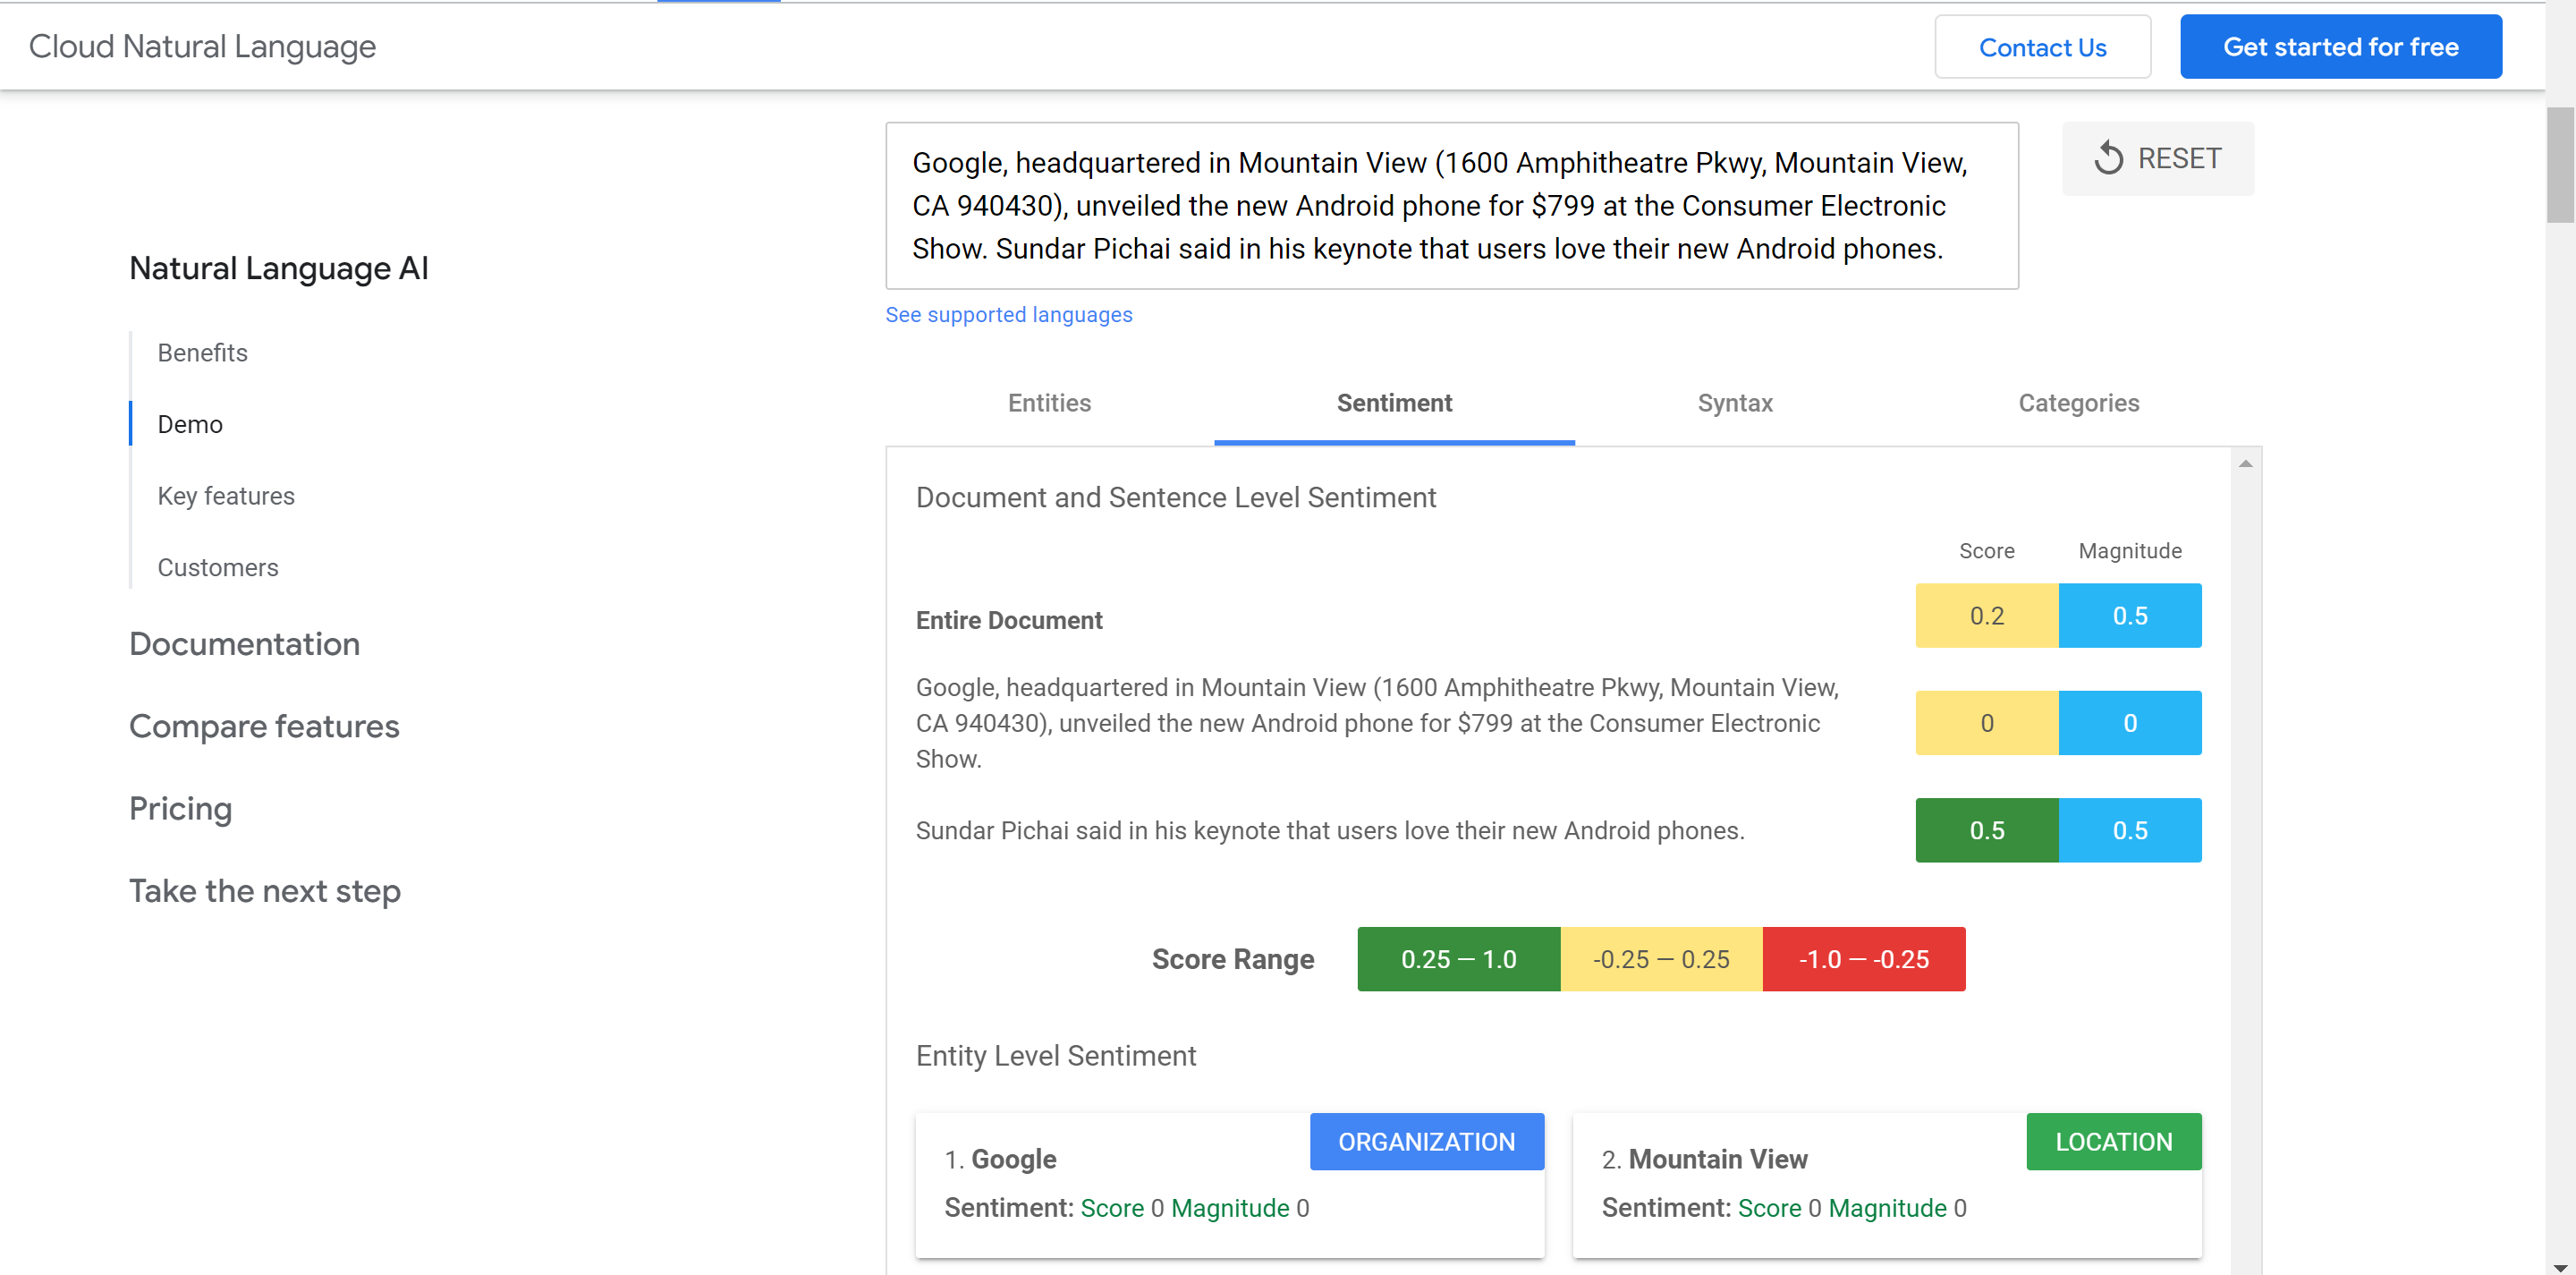
\includegraphics[width=150mm]{figs/googleSearch.png}
    \caption{Servicii Google Cloud Natural Language}
	\label{fig:googleSearch}
\end{figure}
\subsection{Microsoft AI}
{\noindent Acest serviciu are următoarele funcționalități:}
\begin{itemize}
    \setlength\itemsep{0.5em}
    \item Scorul sentimentului pe întreg textul
    \item Extracția entităților, iar acolo unde este posibil, fiecare entitate se află sub un link de Wikipedia
    \item Bing Entity Search oferă un sumar al informațiilor relevante pentru fiecare entitate găsită la punctul anterior
\end{itemize}
\begin{figure}[t]
	\centering
	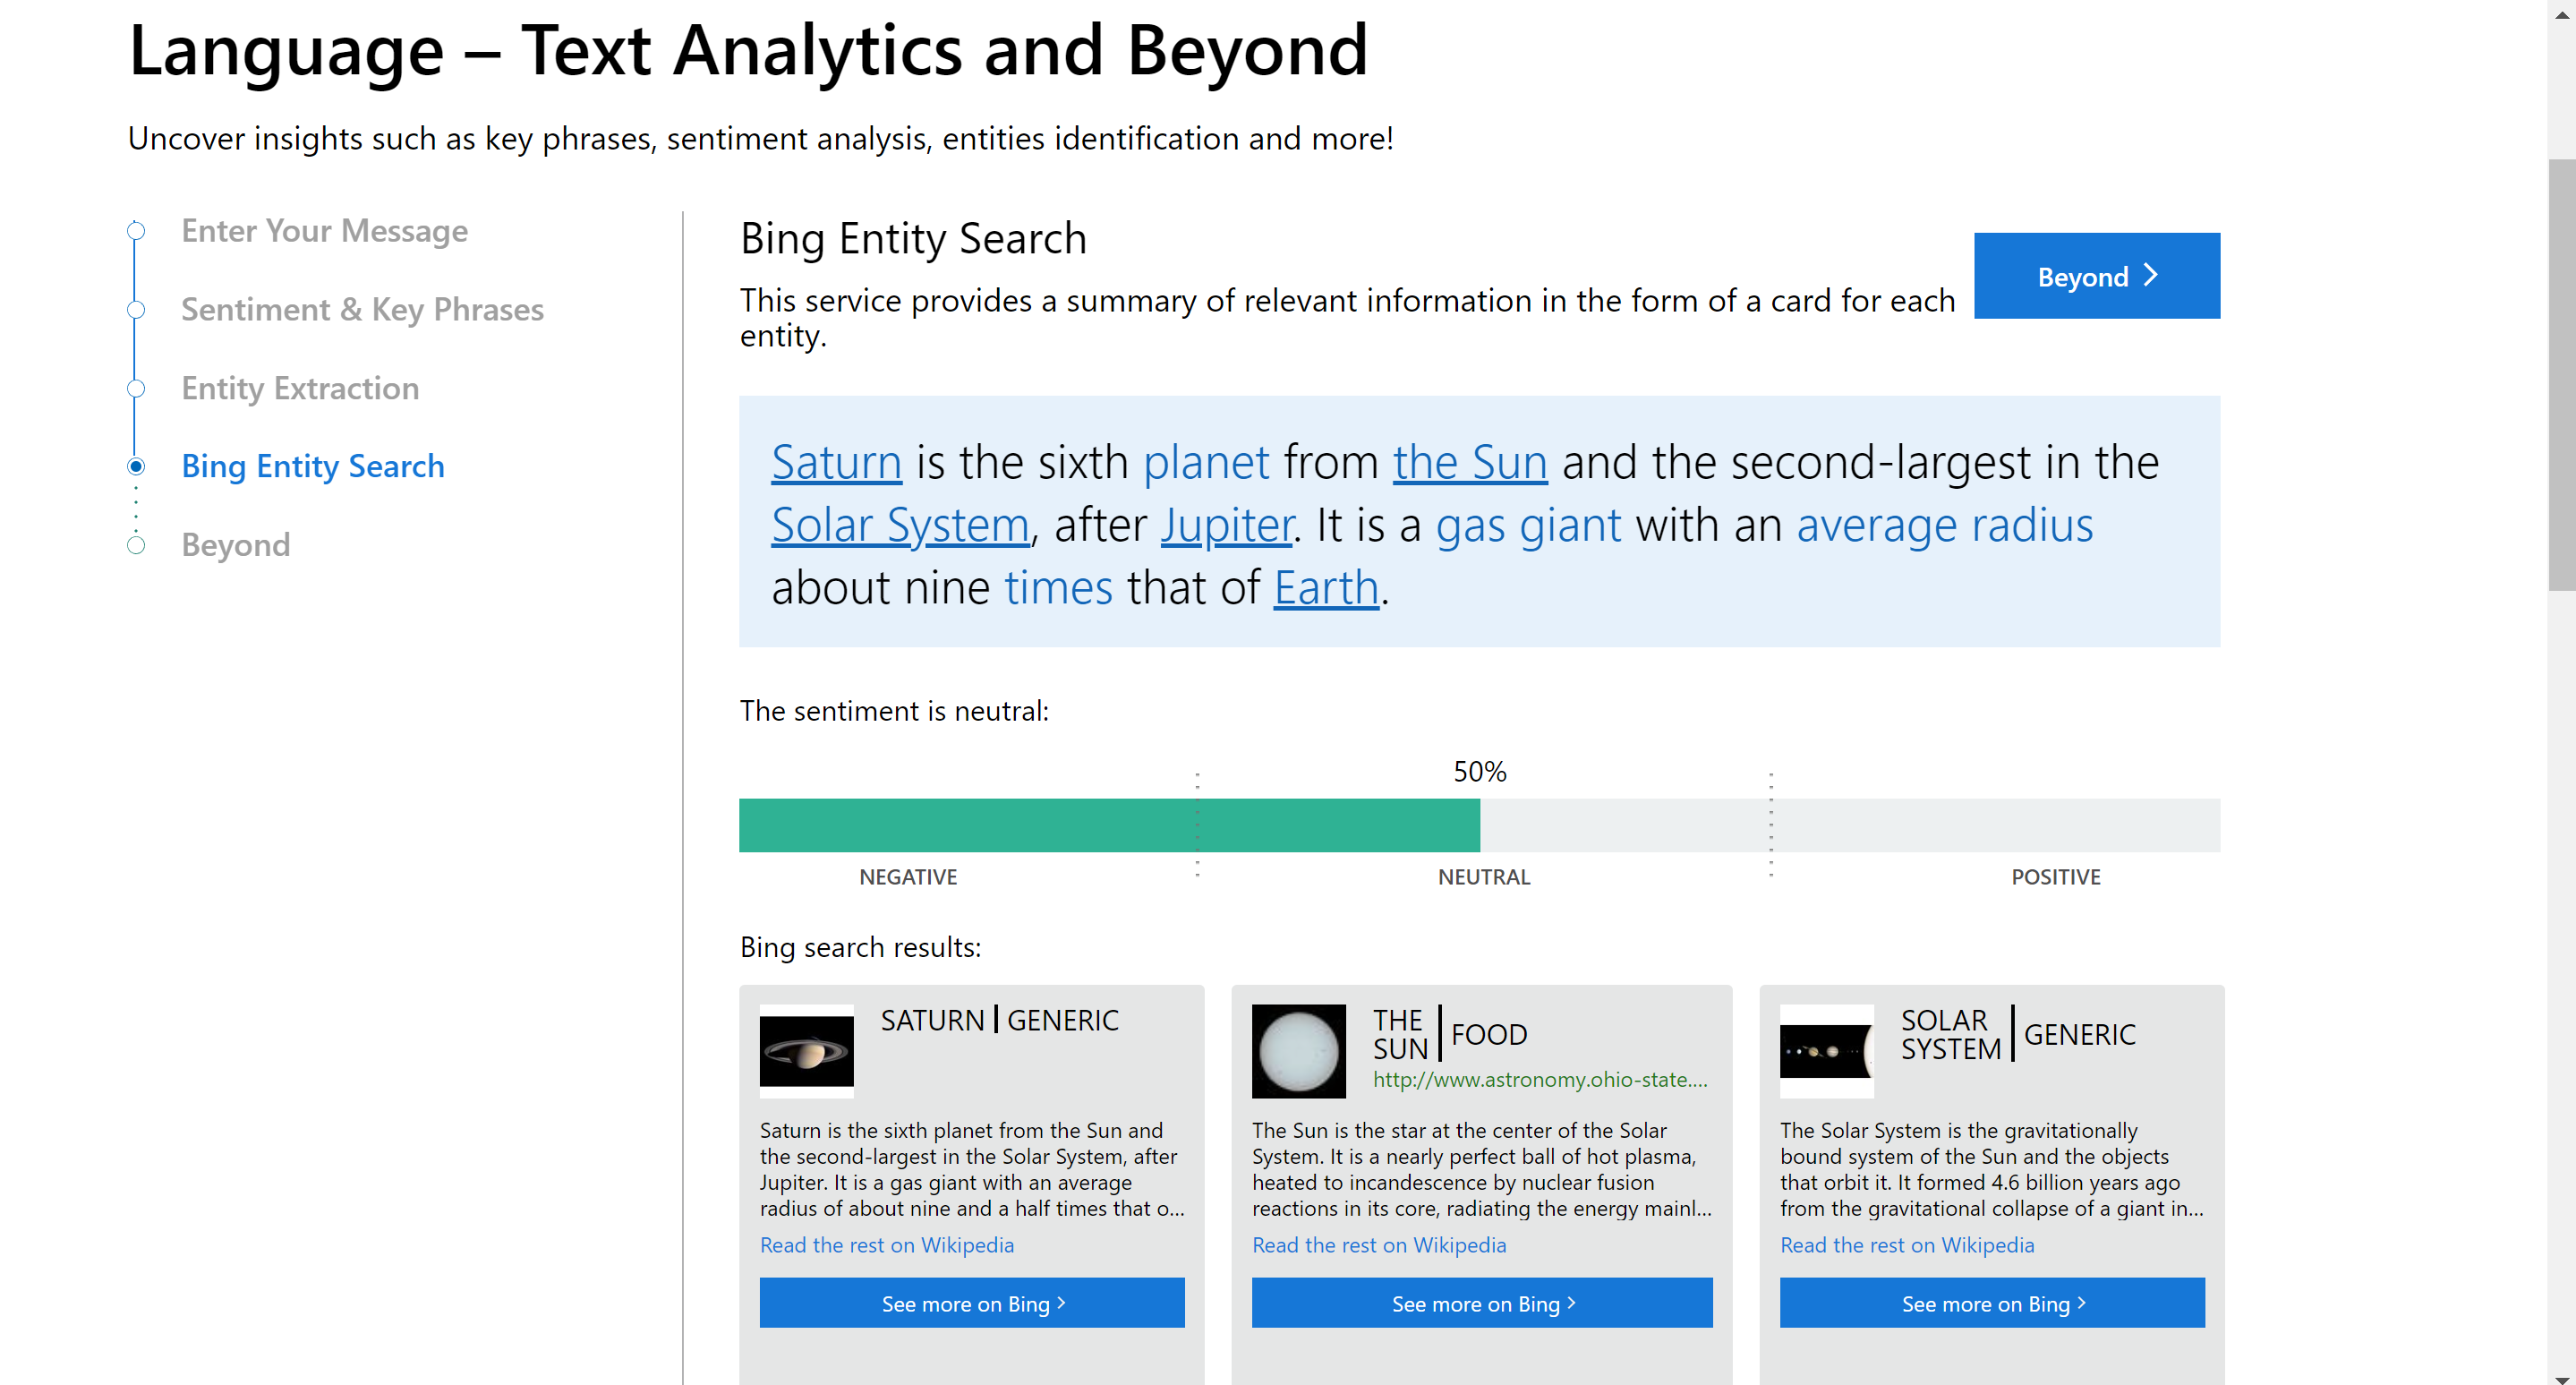
\includegraphics[width=150mm]{figs/msDemo.png}
    \caption{Servicii Microsoft AI}
	\label{fig:msDemo}
\end{figure}
\subsection{Google Trends}
{\noindent Acest serviciu are următoarele funcționalități:}
\begin{itemize}
    \setlength\itemsep{0.5em}
    \item Evoluția unui cuvânt sau a unei expresii într-o perioada de timp, într-o anumită regiune, dintr-o anumită categorie, căutare în mai multe formate
    \item Rezultatele sunt vizuale, afișate pe line chart-uri și hărți
    \item Sugestii de subiecte conexe și căutări similare
    \item Căutări populare zilnice și în timp real
    \item Căutările anului, pe categorii (Oameni, Emisiuni TV, Rețete, Simptome, etc.)
\end{itemize}
\begin{figure}[H]
	\centering
	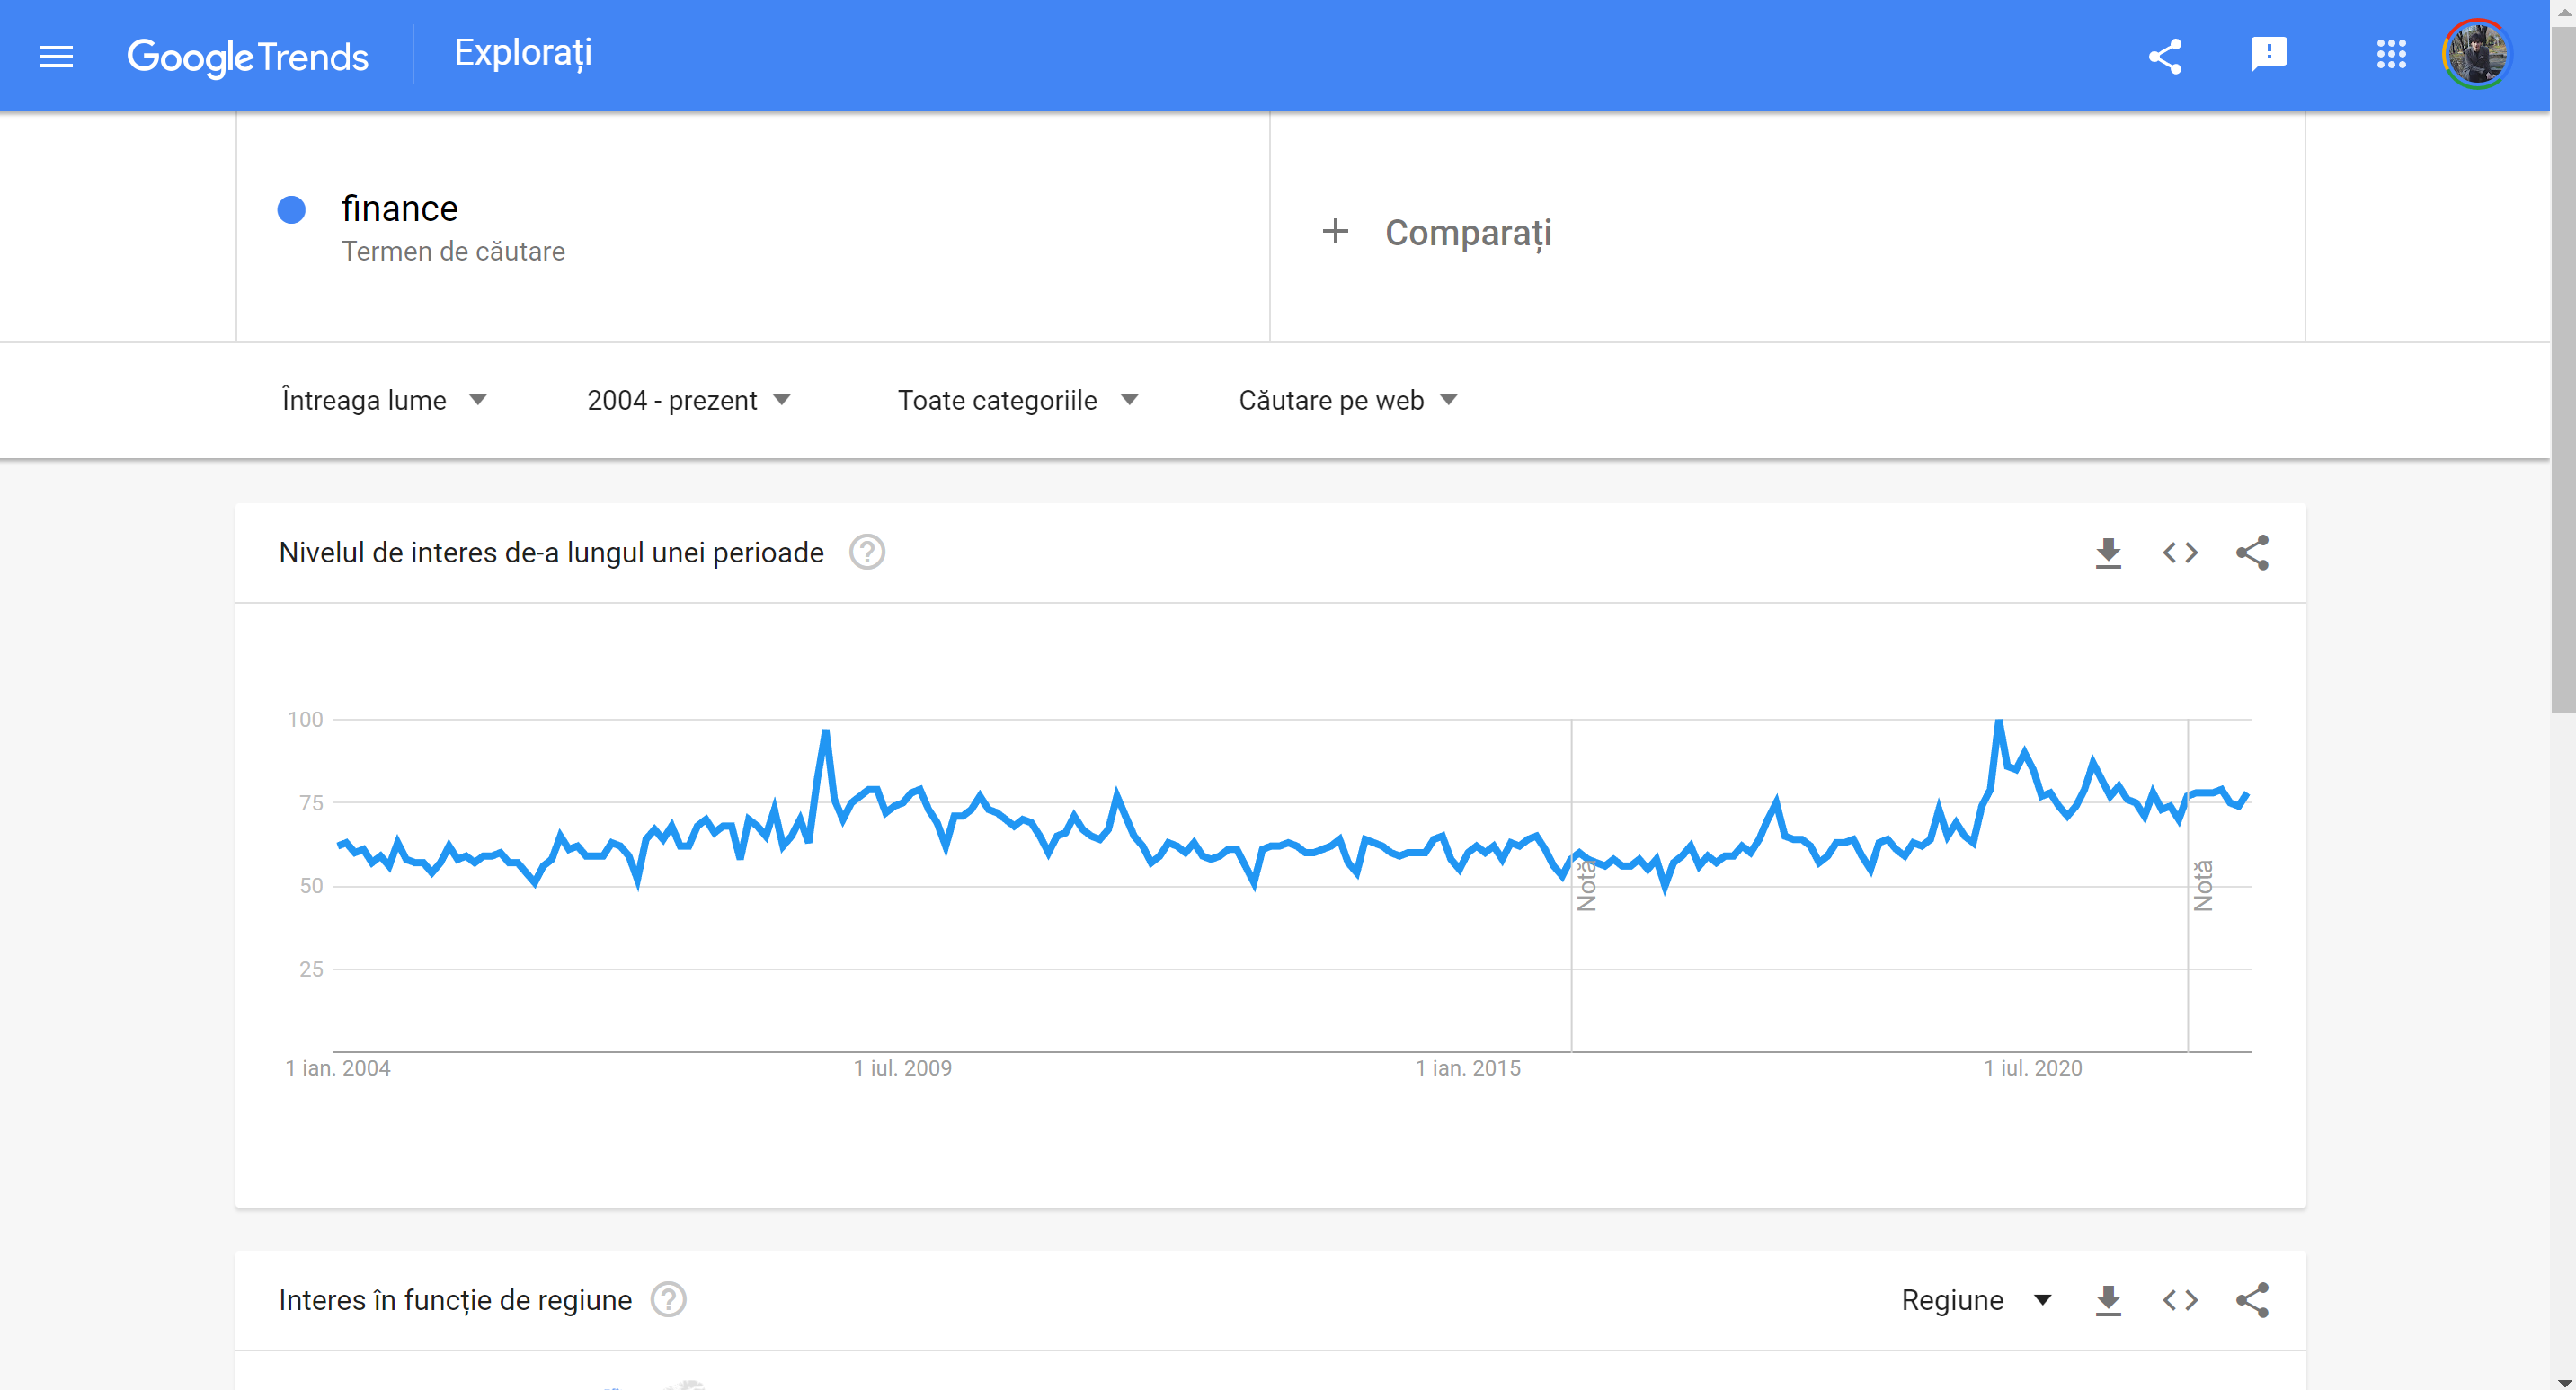
\includegraphics[width=150mm]{figs/googleTrends.png}
    \caption{Servicii Google Trends}
	\label{fig:googleTrends}
\end{figure}



\begin{table}[H]
	\caption{Comparație între aplicația prezentată și ale servicii existente}
	\centering                          % tabel centrat 
	\begin{tabular}{|c|c|c|c|c|c|}          % 4 coloane centrate 
		\hline
		 & IBM & Microsoft AI & Google Search & Google Trends & Aplicație\\ [2ex]   % inserare tabel
		%heading
		\hline                              % linie orizontal simpla
		Serviciu gratuit & NU & NU & NU & DA & DA \\[2ex]               % corpul tabelului 
		Sumarizare & NU & NU & NU & NU & DA \\ [2ex]
        Extracție entități & DA & DA & DA & NU & DA \\ [2ex]
        Analiză sentiment financiar & DA & NU & NU & NU & DA \\[2ex]
        Analiză popularitate & NU & NU & NU & DA & DA \\[2ex]
		Salvare analiză în cont & NU & NU & NU & NU & DA \\[2ex]           % [1ex] adds vertical space
        UI ușor de înțeles și folosit & NU & NU & NU & DA & DA \\[2ex] 
        \hline                              
	\end{tabular}
	% titlul tabelului
	\label{tab:nonlin}                % eticheta folosita pentru referirea tabelului in text; referirea in text se va face cu \ref{table:nonlin}
\end{table} % \chapter{Studiu Bibliografic}

\chapter{Analiză și Fundamentare Teoretică}
\label{ch:analysis}
\pagestyle{fancy}

\section{Cerințe funcționale și non-funcționale}
%%%%%%%%%%%%%%%%%%%%%%%%%%%%%%%%%%%%%%%%%%%%%%%%%%%%%%%%%%%%%%%%%%%%%%%%%%%%%%%%%%%%%%%%%%%%%%%%%%%%%%%%%%%%%%%%%%%%%%%%%%%%%%%%%%%%%%%%%%%%%%%%%%%%%%%%%%
\subsection{Cerințe funcționale}
\begin{itemize}
    \setlength\itemsep{0.5em}
    \item Pentru un utilizator neautentificat, sunt realizabile următoarele acțiuni:
    \begin{itemize}
		\setlength\itemsep{0.5em}
        \item Accesare pagină de Logare
        \item Accesare pagină de Creare cont nou
        \item Încercare de logare
        \item Încercare de creare cont nou
    \end{itemize}
    \item Pentru un utilizator autentificat, sunt realizabile următoarele acțiuni:
    \begin{itemize}
		\setlength\itemsep{0.5em}
        \item Accesare pagină de Dashboard
        \begin{itemize}
            \setlength\itemsep{0.5em}
            \item Adăugare text în caseta de text
            \item Trimitere text spre procesare prin apăsarea butonului de Submit
            \item Vizualizare rezultate
            \item Generare grafic pentru vizualizarea evoluției cuvintelor cheie extrase într-o perioadă de timp selectată de utilizator
            \item Salvare articol (text analizat și rezultatele obținute)
        \end{itemize}
        \item Accesare pagină de Profil
        \begin{itemize}
            \setlength\itemsep{0.5em}
            \item Editare câmp nume
            \item Editare câmp prenume
            \item Editare câmp nume de utilizator, cu condiția să nu fie atribuit altui cont
            \item Editare câmp email, cu condiția să nu fie atribuit altui cont
            \item Editare câmp parolă
        \end{itemize}
        \item Accesare pagina de Trenduri
        \begin{itemize}
            \setlength\itemsep{0.5em}
            \item Generare grafic pentru vizualizarea celor mai populare 10 subiecte într-o perioadă de timp selectată de utilizator
            \item Vizualizarea unui WordCloud, constituit din cuvintele cheie sau expresiile extrase din textele analizate
        \end{itemize}
        \item Accesare pagină de Evoluție
        \begin{itemize}
            \setlength\itemsep{0.5em}
            \item Generare grafic pentru vizualizarea numărului de apariții pentru un cuvânt ales și o perioadă de timp selectată de utilizator
        \end{itemize}
        \item Accesare pagină de Istoric
        \begin{itemize}
            \setlength\itemsep{0.5em}
            \item Vizualizare articole salvate în istoric
            \item Accesarea analizei detaliate a unui articol selectat
            \item Ștergerea unui articol selectat
        \end{itemize}
    \end{itemize}
\end{itemize}
\newpage

\subsection{Cerințe pentru funcții de analiză a unui text}
\begin{itemize}
    \setlength\itemsep{0.5em}
    \item Funcție de analiză a sentimentelor dintr-un text financiar
    \item Funcție de sumarizare a unui text
    \item Funcție de extragere a cuvintelor
\end{itemize}
%%%%%%%%%%%%%%%%%%%%%%%%%%%%%%%%%%%%%%%%%%%%%%%%%%%%%%%%%%%%%%%%%%%%%%%%%%%%%%%%%%%%%%%%%%%%%%%%%%%%%%%%%%%%%%%%%%%%%%%%%%%%%%%%%%%%%%%%%%%%%%%%%%%%%%%%%%
\subsection{Cerințe non-funcționale}
\begin{itemize}
    \setlength\itemsep{0.5em}
    \item Securitatea
    \begin{itemize}
        \setlength\itemsep{0.5em}
        \item Pentru a accesa anumite resurse, utilizatorul trebuie mai întâi să își creeze un cont, apoi să se logheze în aplicație
        \item La crearea contului, înainte să fie salvată, parola trece print-o funcție de hashing cu salt, cu scopul de a avea un rezultat diferit pentru același input al mai multor utilizatori, daca va fi cazul
        \item La logarea în aplicație se generează un token pentru a putea autoriza utilizatorul atunci când dorește să acceseze anumite resurse
    \end{itemize}
    \item Compatibilitatea
    \begin{itemize}
        \setlength\itemsep{0.5em}
        \item Aplicația a fost creată și rulată utilizând ca sistem de operare Windows OS
        \item Pentru a utiliza alt sistem de operare, spre exemplu MacOS, singura diferență este baza de date, fiind necesar găsirea unui echivalent al Microsoft SQL Server Management
    \end{itemize}
\end{itemize}

%%%%%%%%%%%%%%%%%%%%%%%%%%%%%%%%%%%%%%%%%%%%%%%%%%%%%%%%%%%%%%%%%%%%%%%%%%%%%%%%%%%%%%%%%%%%%%%%%%%%%%%%%%%%%%%%%%%%%%%%%%%%%%%%%%%%%%%%%%%%%%%%%%%%%%%%%%

\section{Cazuri de utilizare}
Folosind îndrumările din~\cite{UseCasesGuidlines} pentru crearea și detalierea cazurilor de utilizare a aplicației, trebuie avute în vedere următoarele aspecte: 
\begin{enumerate}
    \setlength\itemsep{0.5em}
    \item {\it Enunțarea precondițiilor}, adică a stării sau stărilor în care sistemul se află înaintea începerii executării operațiunilor specifice cazului de utilizare
    \item {\it Descrierea flow-ului principal}, care trebuie să acopere următoarele: când și unde începe cazul, când cazul de utilizare interacționează cu actorii și când schimbă date, când cazul folosețe date stocate sau dorește să stocheze datele, când și cum este finalizat cazul
    \item {\it Descrierea flow-ului alternativ}, care trebuie să descrie ce se întâmplă cu sistemul în cazurile în care apare o eroare
    \item {\it Enunțarea postcondițiilor}, adică a stării sau stărilor în care sistemul ajunge după ce cazul este finalizat
  \end{enumerate}
%%%%%%%%%%%%%%%%%%%%%%%%%%%%%%%%%%%%%%%%%%%%%%%%%%%%%%%%%%%%%%%%%%%%%%%%%%%%%%%%%%%%%%%%%%%%%%%%%%%%%%%%%%%%%%%%%%%%%%%%%%%%%%%%%%%%%%%%%%%%%%%%%%%%%%%%%%
\subsection{Utilizator neautentificat}

\begin{figure}[h]
	\centering
	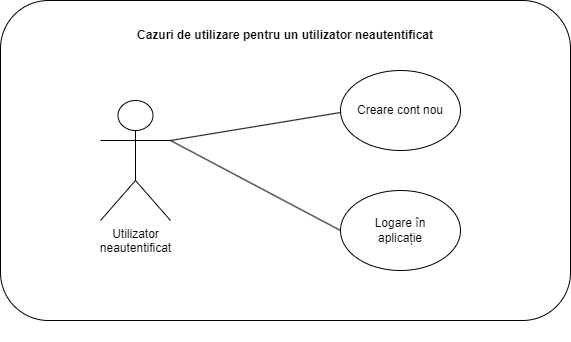
\includegraphics[width=100mm]{figs/useCaseUnauthenticated.png}
    \caption{Cazuri de utilizare pentru un utilizator neautentificat}
	\label{fig:useCaseUnauthenticated}
\end{figure}

\subsubsection{Descrierea cazurilor de utilizare pentru un utilizator neautentificat în figura \ref{fig:useCaseUnauthenticated}}
\begin{enumerate}
    \item Creare cont nou 
    \begin{itemize}
        \setlength\itemsep{0.5em}
        \item Un utilizator neautentificat poate să acceseze pagina de creare cont nou și să se înregistreze în aplicație
        \item Precondiții: utilizatorul neautentificat trebuie să se afle pe pagina de Creare cont nou
        \item Flow principal
        \begin{enumerate}
            \item Utilizatorul neautentificat introduce informațiile necesare: nume, prenume, nume de utilizator, email și parola
            \item Utilizatorul apasă pe butonul de trimitere
            \item Crearea unui nou cont a fost realizată cu succes și utilizatorul este redirecționat la pagina de logare în aplicație
        \end{enumerate}
        \item Flow alternativ
        \begin{enumerate}
            \item Utilizatorul neautentificat introduce informațiile necesare: nume, prenume, nume de utilizator, email și parola
            \item Utilizatorul apasă pe butonul de trimitere
            \item Emailul sau numele de utilizator deja sunt folosite de alt cont
            \item Flow-ul este reluat
        \end{enumerate}
        \item Postcondiții: Dacă a fost creat cu succes contul, utilizatorul este redirecționat la pagina de logare în aplicație
    \end{itemize}

    \item Logare
    \begin{itemize}
        \setlength\itemsep{0.5em}
        \item Un utilizator neautentificat poate să acceseze pagina de logare și să intre în aplicație, dacă acesta are deja un cont creat
        \item Precondiții: utilizatorul neautentificat trebuie să se afle pe pagina de logare
        \item Flow principal
        \begin{enumerate}
            \item Utilizatorul neautentificat introduce informațiile necesare: nume de utilizator sau email și parola
            \item Utilizatorul apasă pe butonul de trimitere
            \item Logarea s-a făcut cu succes și utilizatorul este acum autentificat și redirecționat la pagina de Dashboard
        \end{enumerate}
        \item Flow alternativ
        \begin{enumerate}
            \item Utilizatorul neautentificat introduce informațiile necesare: nume de utilizator sau email și parola
            \item Utilizatorul apasă pe butonul de trimitere
            \item Credențialele sunt greșite
            \item Flow-ul este reluat
        \end{enumerate}
        \item Postcondiții: Dacă utilizatorul s-a logat în aplicație, este redirecționat la pagina de Dashboard
    \end{itemize}
  \end{enumerate}

%%%%%%%%%%%%%%%%%%%%%%%%%%%%%%%%%%%%%%%%%%%%%%%%%%%%%%%%%%%%%%%%%%%%%%%%%%%%%%%%%%%%%%%%%%%%%%%%%%%%%%%%%%%%%%%%%%%%%%%%%%%%%%%%%%%%%%%%%%%%%%%%%%%%%%%%%%
\newpage
\subsection{Utilizator autentificat}
\begin{figure}[ht]
	\centering
	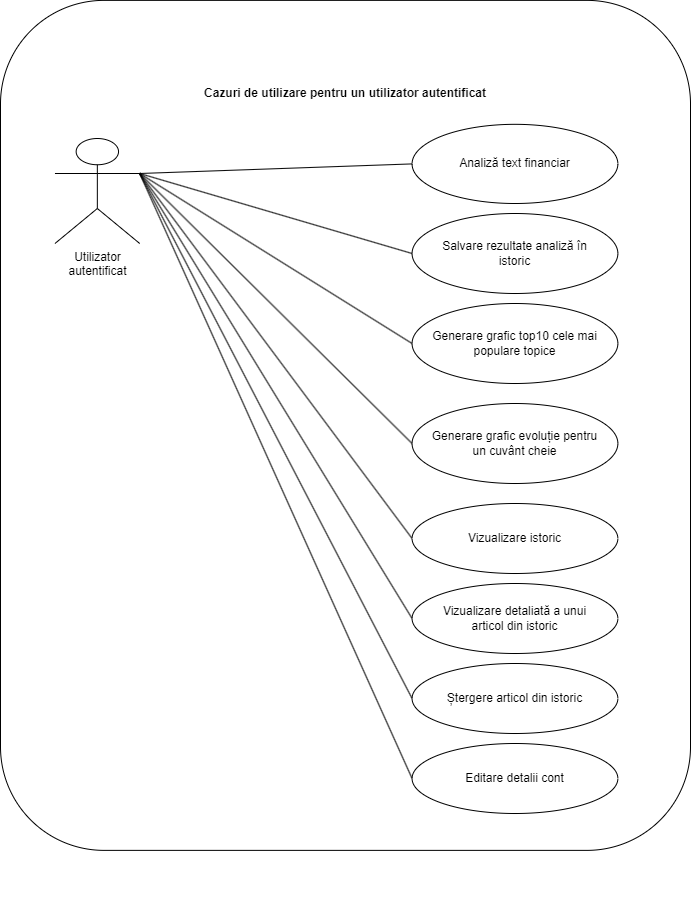
\includegraphics[width=100mm]{figs/useCasesAuthenticated.png}
    \caption{Cazuri de utilizare pentru un utilizator autentificat}
	\label{fig:useCasesAuthenticated}
\end{figure}
\subsubsection{Descrierea cazurilor de utilizare pentru un utilizator autentificat în figura \ref{fig:useCasesAuthenticated}}
\begin{enumerate}
    \setlength\itemsep{0.5em}
    \item Analizare text financiar
    \begin{itemize}
        \setlength\itemsep{0.5em}
        \item Un utilizator autentificat poate să introducă un text financiar și să îl obțină o analiză detaliată
        \item Precondiții: utilizatorul autentificat trebuie să se afle pe pagina de Dashboard
        \item Flow principal
        \begin{enumerate}
            \setlength\itemsep{0.5em}
            \item Utilizatorul autentificat introduce textul
            \item Utilizatorul apasă pe butonul de trimitere
            \item Apare un buton pentru a-l trimite pe utilizator într-o pagină cu rezultatele obținute în urma analizei
        \end{enumerate}
        \item Flow alternativ
        \begin{enumerate}
            \setlength\itemsep{0.5em}
            \item Utilizatorul autentificat introduce textul
            \item Utilizatorul apasă pe butonul de trimitere
            \item Modelul care trebuie să transmită rezultatele încă se încarcă
            \item Flow-ul este reluat
        \end{enumerate}
        \item Postcondiții: Dacă textul a fost analizat și apare butonul care îl trimite pe utilizator într-o pagină cu rezultatele obținute în urma analizei
    \end{itemize}

    \item Salvare rezultate analiză în istoric
    \begin{itemize}
        \setlength\itemsep{0.5em}
        \item Un utilizator autentificat poate să salveze rezultatele detaliate ale analizei textului
        \item Precondiții: utilizatorul autentificat trebuie să se afle în pagina de Dashboard, în partea cu toate informațiile detaliate
        \item Flow principal
        \begin{enumerate}
            \setlength\itemsep{0.5em}
            \item Utilizatorul autentificat apasă pe butonul de salvare
            \item Se deschide un modal pentru confirmare
            \item Se confirmă și articoul analizat este salvat în istoricul utilizatorului
        \end{enumerate}
        \item Postcondiții: Dacă utilizatorul a salvat articolul, acesta va apărea în tabelul din pagina de istoric
    \end{itemize}
\ \\
    Diagrama FlowChart se găsește în figura \ref{fig:saveArticleFlowchart}.
    \begin{figure}[H]
        \centering
        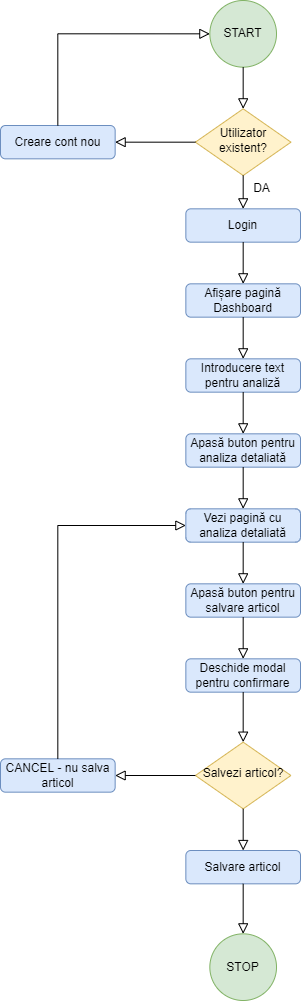
\includegraphics[height=100mm]{figs/saveArticleFlowchart.png}
        \caption{Diagramă FlowChart pentru salvarea rezultatelor unui text analizat în istoric}
        \label{fig:saveArticleFlowchart}
    \end{figure}

    \item Generare grafic pentru top 10 cele mai populare subiecte din aplicație
    \begin{itemize}
        \setlength\itemsep{0.5em}
        \item Un utilizator autentificat poate să genereze un grafic pentru a vedea top 10 cele mai populare cuvinte cheie (subiecte) din aplicație
        \item Precondiții: utilizatorul autentificat trebuie să se afle în pagina de Trending
        \item Flow principal
        \begin{enumerate}
            \setlength\itemsep{0.5em}
            \item Utilizatorul autentificat selectează o perioadă
            \item Utilizatorul apasă pe butonul de trimitere
            \item Apar rezultatele pe grafic
        \end{enumerate}
        \item Flow alternativ
        \begin{enumerate}
            \setlength\itemsep{0.5em}
            \item Utilizatorul autentificat selectează o perioadă
            \item Utilizatorul apasă pe butonul de trimitere
            \item Utilizatorul este notificat că nu există date din perioada selectată de acesta
            \item Flow-ul este reluat, selectând altă perioadă
        \end{enumerate}
        \item Postcondiții: Utilizatorul rămâne în pagina de Trending, având posibilitatea selectării altei perioade
    \end{itemize}

    \ \\
    Diagrama FlowChart se găsește în figura \ref{fig:trends}.
    \begin{figure}[H]
        \centering
        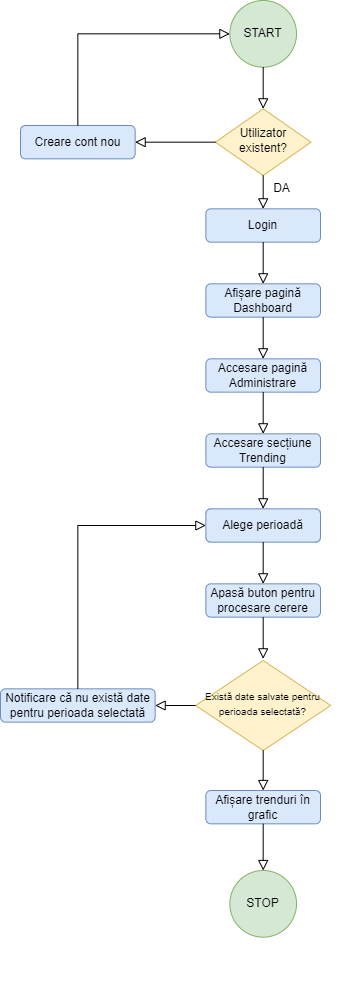
\includegraphics[height=100mm]{figs/trends.png}
        \caption{Diagramă FlowChart pentru generare grafic cu top 10 trenduri în aplicație}
        \label{fig:trends}
    \end{figure}

    \item Generare grafic pentru a vizualiza evoluția unui cuvânt cheie, într-o anumită perioadă
    \begin{itemize}
        \setlength\itemsep{0.5em}
        \item Un utilizator autentificat poate să genereze un grafic pentru a vedea evoluția unui cuvânt cheie, într-o anumită perioadă
        \item Precondiții: utilizatorul autentificat trebuie să se afle în pagina de Evoluție
        \item Flow principal
        \begin{enumerate}
            \setlength\itemsep{0.5em}
            \item Utilizatorul autentificat selectează o perioadă
            \item Utilizatorul autentificat introduce cuvântul
            \item Utilizatorul apasă pe butonul de trimitere
            \item Apar rezultatele pe grafic
        \end{enumerate}
        \item Flow alternativ
        \begin{enumerate}
            \setlength\itemsep{0.5em}
            \item Utilizatorul autentificat selectează o perioadă
            \item Utilizatorul autentificat introduce cuvântul
            \item Utilizatorul apasă pe butonul de trimitere
            \item Utilizatorul este notificat că nu există date, posibil din cauza perioadei sau din cauză că până acum nu a mai fost căutat cuvântul
            \item Flow-ul este reluat, selectând altă perioadă
        \end{enumerate}
        \item Postcondiții: Utilizatorul rămâne în pagina de Evoluție, având posibilitatea selectării altei perioade sau introducerii altui cuvânt
    \end{itemize}

    \item Vizualizare istoric
    \begin{itemize}
        \setlength\itemsep{0.5em}
        \item Un utilizator autentificat poate să vizualizeze istoricul
        \item Precondiții: utilizatorul autentificat poate să se afle în orice pagină
        \item Flow principal
        \begin{enumerate}
            \setlength\itemsep{0.5em}
            \item Utilizatorul autentificat selectează din bara de nagivare butonul de Istoric
            \item Utilizatorul este redirecționat la pagina de Istoric, unde poate vedea tabelul cu articolele salvate până acum
        \end{enumerate}
        \item Postcondiții: Utilizatorul este redirecționat la pagina de Istoric, unde poate vedea tabelul cu articolele salvate până acum
    \end{itemize}

    \item Vizualizarea detaliată a unui articol din istoric
    \begin{itemize}
        \setlength\itemsep{0.5em}
        \item Un utilizator autentificat poate să vizualizeze mai multe detalii ale unui articol salvat în istoric
        \item Precondiții: utilizatorul autentificat trebuie să se afle în pagina de Istoric
        \item Flow principal
        \begin{enumerate}
            \setlength\itemsep{0.5em}
            \item Utilizatorul autentificat apasă pe butonul de Vezi mai mult din dreptul articolului pe care dorește să îl redeschidă
            \item Apare un modal de confirmare
            \item Utilizatorul confirmă că vrea să revadă analiza acelui articol
            \item Utilizatorul este redirecționat în pagina de Dashboard, de această dată fără opțiunea de a salva articolul (pentru că acesta deja există în istoric)
        \end{enumerate}
        \item Flow alternativ
        \begin{enumerate}
            \setlength\itemsep{0.5em}
            \item Utilizatorul autentificat apasă pe butonul de Vezi mai mult din dreptul articolului pe care dorește să îl redeschidă
            \item Apare un modal de confirmare
            \item Utilizatorul nu confirmă că vrea să revadă analiza acelui articol
            \item Utilizatorul rămâne în pagina de Istoric
        \end{enumerate}
        \item Postcondiții: Utilizatorul este direcționat în pagina cu analiza detaliată a articolului selectat
    \end{itemize}


    \item Ștergere a unui articol din istoric
    \begin{itemize}
        \setlength\itemsep{0.5em}
        \item Un utilizator autentificat poate să șteargă un articol salvat în istoric
        \item Precondiții: utilizatorul autentificat trebuie să se afle în pagina de Istoric
        \item Flow principal
        \begin{enumerate}
            \setlength\itemsep{0.5em}
            \item Utilizatorul autentificat apasă pe butonul de Șterge din dreptul articolului pe care dorește să îl redeschidă
            \item Apare un modal de confirmare
            \item Utilizatorul confirmă că vrea să șteargă articolul
            \item Articolul este șters și tabelul este actualizat
        \end{enumerate}
        \item Flow alternativ
        \begin{enumerate}
            \setlength\itemsep{0.5em}
            \item Utilizatorul autentificat apasă pe butonul de Șterge din dreptul articolului pe care dorește să îl redeschidă
            \item Apare un modal de confirmare
            \item Utilizatorul nu confirmă că vrea să șteargă articolul
            \item Utilizatorul rămâne în pagina de Istoric și tabelul nu este actualizat
        \end{enumerate}
        \item Postcondiții: Se actualizează tabelul din istoricul utilizatorului și rămâne în pagina de Istoric
    \end{itemize}

    \ \\
    Diagrama FlowChart se găsește în figura \ref{fig:deleteArticle}.
    \begin{figure}[H]
        \centering
        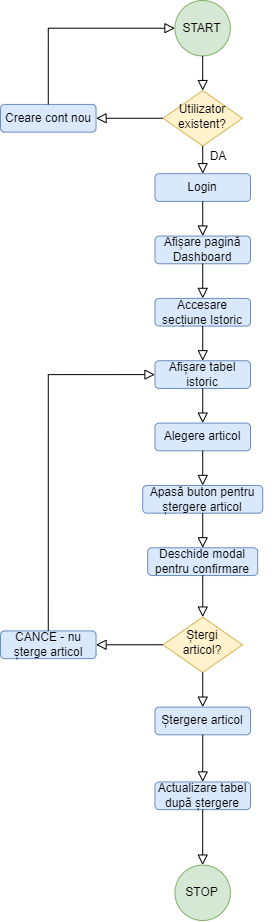
\includegraphics[height=110mm]{figs/deleteArticle.png}
        \caption{Diagramă FlowChart pentru ștergere articol din istoric}
        \label{fig:deleteArticle}
    \end{figure}

    \item Editare detalii cont
    \begin{itemize}
        \setlength\itemsep{0.5em}
        \item Un utilizator autentificat poate să editeze detaliile contului
        \item Precondiții: utilizatorul autentificat trebuie să se afle în pagina de Profil
        \item Flow principal
        \begin{enumerate}
            \setlength\itemsep{0.5em}
            \item Utilizatorul autentificat editează unul sau mai multe din câmpurile: nume, prenume, nume de utilizator, email, parolă nouă și confirmă parola
            \item Utilizatorul apasă pe butonul de trimitere
            \item Utilizatorul este notificat că detaliile contului au fost modificate cu succes
        \end{enumerate}
        \item Flow alternativ
        \begin{enumerate}
            \setlength\itemsep{0.5em}
            \item Utilizatorul autentificat editează unul sau mai multe din câmpurile: nume, prenume, nume de utilizator, email, parolă nouă și confirmă parola
            \item Unul dintre câmpurile de email sau nume de utilizator este deja folosit de alt cont
            \item Utilizatorul apasă pe butonul de trimitere
            \item Utilizatorul este notificat că email-ul sau numele de utilizator este deja folosit de alt cont
            \item Flow-ul este reluat
        \end{enumerate}
        \item Postcondiții: Detaliile contului au fost modificate cu succes
    \end{itemize}
  \end{enumerate}


%%%%%%%%%%%%%%%%%%%%%%%%%%%%%%%%%%%%%%%%%%%%%%%%%%%%%%%%%%%%%%%%%%%%%%%%%%%%%%%%%%%%%%%%%%%%%%%%%%%%%%%%%%%%%%%%%%%%%%%%%%%%%%%%%%%%%%%%%%%%%%%%%%%%%%%%%%
%%%%%%%%%%%%%%%%%%%%%%%%%%%%%%%%%%%%%%%%%%%%%%%%%%%%%%%%%%%%%%%%%%%%%%%%%%%%%%%%%%%%%%%%%%%%%%%%%%%%%%%%%%%%%%%%%%%%%%%%%%%%%%%%%%%%%%%%%%%%%%%%%%%%%%%%%%

\section{Algoritmi utilizați}
\subsection{Algoritmul pentru autorizarea accesului utilizatorului la anumite resurse}
Atunci când un utilizator nou își creează un cont și se loghează în aplicație, identitatea acestuia este verificată printr-un proces de autentificare. \\
Pentru a accesa anumite resurse, acesta trebuie să fie autorizat. Spre exemplu, pentru e efectua operații de ștergere a unor elemente importante, utilizatorul trebuie să aibă permisiunile necesare.
Așadar, pentru partea de autorizare utilizator, mecanismul este următorul: în momentul în care clientul trimite un request de logare în aplicație, se returnează un token pentru autorizarea requesturilor viitoare, dacă nu există deja unul. \\

Validarea tokenului pentru un anumit utilizator depinde de utilizator (pentru că serviciul folosește un map cu userId și token), de valabilitatea tokenului și dacă valoarea stocată în map corespunde cu valoarea transmisă pentru verificare. 
Dacă toate cele 3 condiții sunt îndeplinite, utilizatorul are permisiunea de a efectua operația pentru care s-a făcut această verificare.

\subsection{Algoritmul pentru crearea unei parole puternice}
O funcție de hashing este folosită pentru a lua un mesaj de o orice lungime, apoi în urma procesării, va rezulta un răspuns de lungime fixă.
Spre exemplu, funcția de hashing SHA512 va produce o valoarea de 512 biți, indiferent de lungimea valorii de intrare. Această funcție a fost folosită pentru a asigura securitatea parolei la înregistrarea unui utilizator nou.\\

Problema la funcțiile de hashing apare pentru că același input va produce același output de lungime fixă. 
Pentru a asigura unicitatea rezultatului, se folosește un {\it salt}, un set de caractere care sunt adăugate la finalul parolei, în acest caz, înainte să treacă prin funcția de hashing.


%%%%%%%%%%%%%%%%%%%%%%%%%%%%%%%%%%%%%%%%%%%%%%%%%%%%%%%%%%%%%%%%%%%%%%%%%%%%%%%%%%%%%%%%%%%%%%%%%%%%%%%%%%%%%%%%%%%%%%%%%%%%%%%%%%%%%%%%%%%%%%%%%%%%%%%%%%

\section{Protocoale utilizate}
\subsection{Protocolul HTTP}
Protocolul HTTP este un protocol utilizat pentru a transmite date între un server Web și un broswer (Google Chrome, Firefox, etc.). Se bazează pe protocolul de comunicare TCP/IP.\\
Se bazează pe mecanismul request-response, unde clientul (în acest caz, browserul) inițiază un request, apoi așteaptă un răspuns de la server.\\
Serverul procesează requestul primit de la client, apoi trimite răspunsul, după care conexiunea se întrerupe. Așadar, clientul și serverul sunt conectați doar pentru requestul și răspunsul curent, concluzionând astfel că 
protocolul HTTP este un protocol fără conexiune.\\
Tot din acest motiv, clientul și serverul nu rețin informații unul despre celalălalt, concluzionând că protocolul HTTP este un protocol fără stare, după cum putem afla din ~\cite{HTTPDefinition}.
\begin{figure}[H]
	\centering
	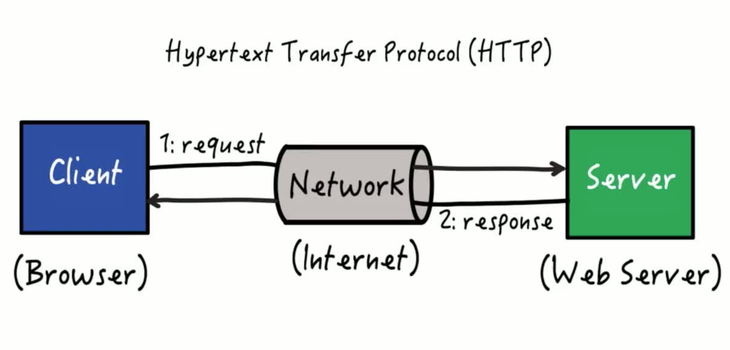
\includegraphics[width=100mm, scale=1]{figs/http.png}
    \caption{Protocolul HTTP. Sursa~\cite{HTTPDiagram}}
	\label{fig:http}
\end{figure}

\subsection{Protocolul TCP/IP}
Pentru SQL Server, protocolul TCP/IP se utilizează cel mai des, pentru că acesta permite dispozitivelor să comunice între diferite dispozitive.\\
De fiecare dată când se trimite ceva prin intermediul Internetului, modelul TCP/IP structurează informația în pachete pe care apoi le transmite prin cele 4 nivele: Aplicație, Transport, Internet, Acces rețea.
Informațiile sunt trimise în ordine, apoi sunt reasamblate în ordine inversă la celalalt capăt, așa cum este menționat aici~\cite{TCPDefinition}.\\

Protocolul TCP stabilește o conexiune între host-uri (server și baza de date, în acest caz), apoi asigură că pachetele de date sunt livrate.
\begin{figure}[H]
	\centering
	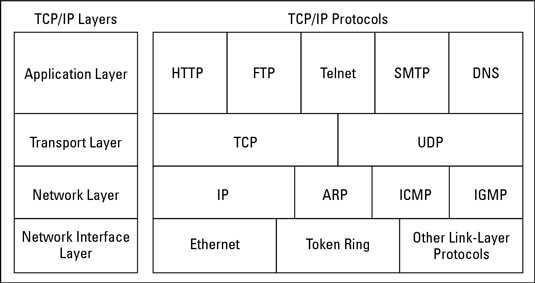
\includegraphics[width=100mm, scale=1]{figs/tcp.jpg}
    \caption{Modelul TCP/IP. Sursa~\cite{TCPDiagram}}
	\label{fig:tcp}
\end{figure}

%%%%%%%%%%%%%%%%%%%%%%%%%%%%%%%%%%%%%%%%%%%%%%%%%%%%%%%%%%%%%%%%%%%%%%%%%%%%%%%%%%%%%%%%%%%%%%%%%%%%%%%%%%%%%%%%%%%%%%%%%%%%%%%%%%%%%%%%%%%%%%%%%%%%%%%%%%
\subsection{Protocolul SMTP}
SMTP sau Simple Mail Transfer Protocol, este un protocol de email utilizat pentru a trimite mesaje dintr-un cont de email în altul, prin intermediul Internetului, bazat pe adresele de email.\\
Permite trimiterea unui mesaj spre unul sau mai mulți destinatari, includerea atașamentelor precum text, video, fotografii.\\
Atunci când un mail este trimis de la un client, acesta va ajunge la un server SMTP care e responsabil pentru transmiterea email-urilor mai departe, spre destinatar (serverul de mail al destinatarului).\\
De fiecare data când un mail este trimis, o conexiune se va deschide între serverul SMTP și serverul destinatar, care va asigura transmiterea datelor spre un destinatar valid. Altfel, email-ul revine la expeditor.
\begin{figure}[H]
	\centering
	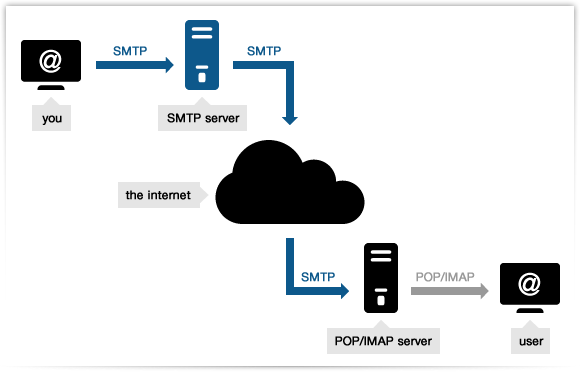
\includegraphics[width=100mm, scale=1]{figs/smtp.png}
    \caption{Protocolul SMTP. Sursa~\cite{SMTP}}
	\label{fig:smtp}
\end{figure} % \chapter{Analiză și Fundamentare Teoretică}

\chapter{Proiectare de Detaliu și Implementare}
\pagestyle{fancy}

\section{Structura aplicației}
Aplicația se bazează pe arhitectura client-server, folosind un mecanism de comunicare request-response. Clientul trimite un request spre server, iar serverul procesează cererea clientului și trimite un răspuns către acesta.
Utilizarea acestui tip de arhitectură are următoarele avantaje, cum sunt menționate aici~\cite{CSAdvantages}
\begin{itemize}
	\setlength\itemsep{0.5em}
	\item Centralizarea informațiilor
	\begin{itemize}
		\setlength\itemsep{0.5em}
		\item Toate informațiile necesare pot fi găsite într-un loc
	\end{itemize}
	\item Scalabilitatea
	\begin{itemize}
		\setlength\itemsep{0.5em}
		\item Numărul de clienți și servere poate fi ușor extins
		\item Chiar dacă numărul clienților sau al serverelor crește, nu reprezintă nicio problemă pentru că totul este deja centralizat și poate fi găsit și accesat cu ușurință de către persoanele autorizate
	\end{itemize}
	\item Securitatea
	\begin{itemize}
		\setlength\itemsep{0.5em}
		\item Sistemul este bine protejat, putând adauga anumite drepturi de acces pentru utilizatori
	\end{itemize}
\end{itemize}

Un tip de arhitectură client-server este {\it Arhitectura 3-tier} sau Arhitectura pe 3 nivele. Acestea sunt: nivelul prezentare, fiind reprezentat de partea de interfață cu utilizatorul, nivelul aplicație,
care cuprinde partea de logică și nivelul de date, care reprezintă mediul de stocare.\\
Nivelul de prezentare, de fapt, este reprezentat de partea de client a sistemului, iar partea de aplicație este reprezentată de partea de server alături de baza de date pentru a putea efectua diferite operații.\\

Partea de client a fost implementată utilizând React Typescript, iar partea de server a fost implementată utilizând ASP.NET Core. Pentru baza de date s-a utilizat Microsoft SQL Server Management Studio.\\

Clientul interacționează cu serverul folosind protocolul de comunicare HTTP. Acesta trimite request-uri spre server, urmând a fi procesate și returnat un răspuns. Pentru procesarea anumitor request-uri venite de la client,
serverul interacționează și cu baza de date, folosind ca protocol de comunicare TCP/IP. \\
Operațiile pe care serverul le poate realiza la nivelul bazei de date constă în operații de stocare, citire a datelor deja stocate, actualizare a datelor și ștergere. \\

\noindent În figura \ref{fig:conceptualArchitecture} este reprezentată diagrama conceptuală a aplicației.
\begin{figure}[H]
	\centering
	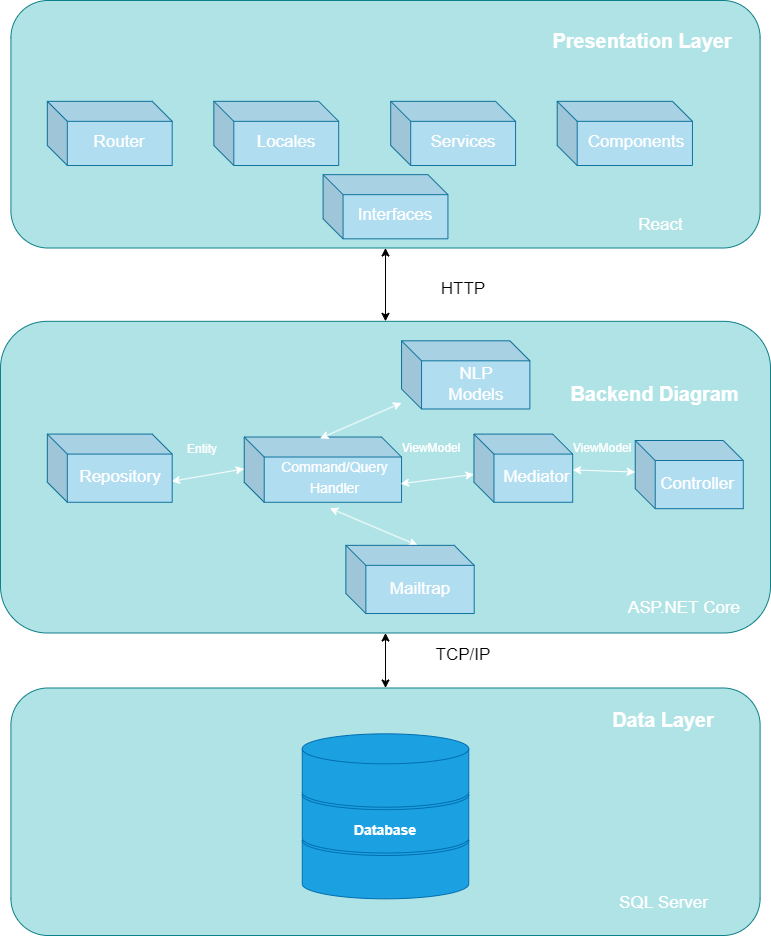
\includegraphics[height=200mm]{figs/conceptualArchitecture.png}
	\caption{Arhitectura conceptuală a sistemului}
	\label{fig:conceptualArchitecture}
\end{figure}
\newpage

\section{Structura bazei de date}
În figura \ref{fig:dbDiagram} este reprezentată diagrama bazei de date. Această diagramă a fost creată cu ajutorul dbdiagram.io~\cite{DbDiagram}
\begin{figure}[H]
	\centering
	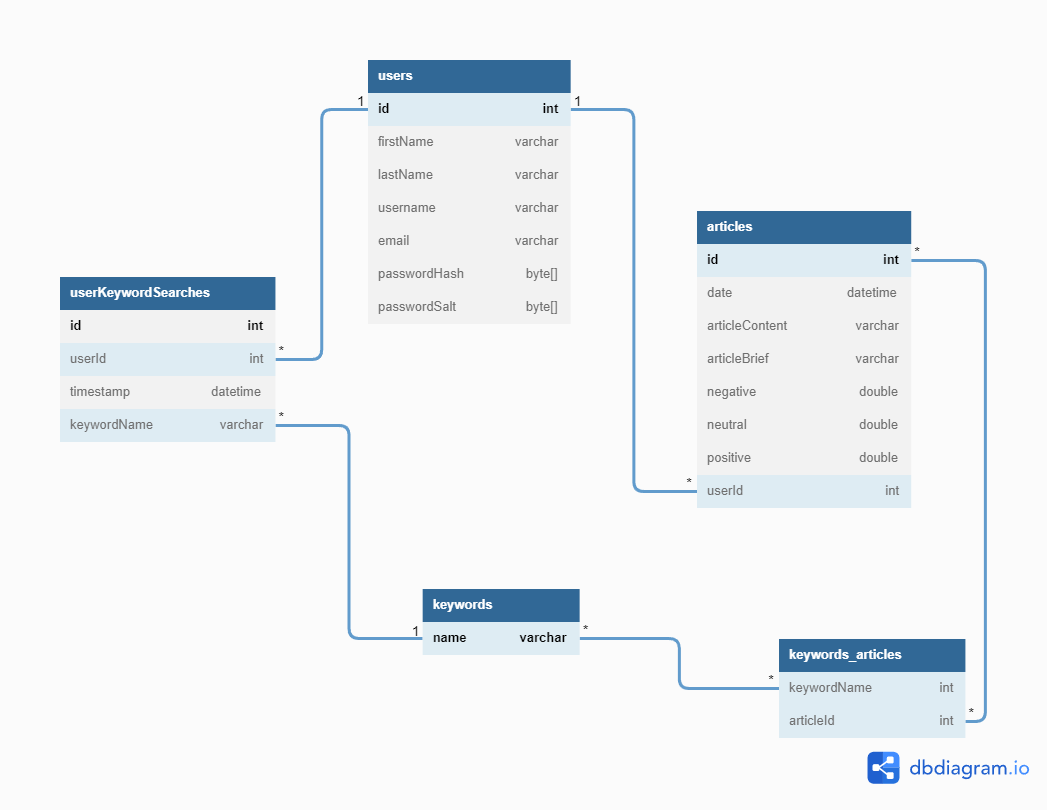
\includegraphics[width=150mm]{figs/dbDiagram.png}
	\caption{Diagrama bazei de date}
	\label{fig:dbDiagram}
\end{figure}

Tabelele din baza de date sunt următoarele: Users, Keywords, UserKeywordSearches, Articles și o tabelă pentru a ilustra relația dintre Keywords și Articles.
\subsubsection{Tabela Users}
Această tabelă conține informațiile despre un utilizator.
\begin{itemize}
	\setlength\itemsep{0.5em}
	\item Id - reprezintă Id-ul utilizatorului, un identificator unic și este cheie primară în acest tabel
	\item FirstName - reprezintă prenumele utilizatorului, nu poate fi null și nu include caractere speciale sau cifre
	\item LastName - reprezintă numele utilizatorului, nu poate fi null și nu include caractere speciale sau cifre
	\item Email - reprezintă email-ul utilizatorului, nu poate avea duplicat, trebuie să aiba formatul corect pentru email
	\item Username - reprezintă numele de utilizator, nu poate fi null, poate avea caractere speciale sau cifre
	\item PasswordHash și PasswordSalt - reprezintă parola utilizatorului (explicată în partea de nivel de aplicație), nu poate fi null
\end{itemize}

\subsubsection{Tabela Keywords}
Această tabelă conține informațiile despre un keyword.
\begin{itemize}
	\setlength\itemsep{0.5em}
	\item Name - reprezintă identificatorul keyword-ului (cuvântului cheie sau frazei) și este cheie primară în acest tabel
\end{itemize}

\subsubsection{Tabela UserKeywordSearches}
Această tabelă conține informațiile despre un cuvânt cheie sau expresie identificată în textul analizat de utilizator.
\begin{itemize}
	\setlength\itemsep{0.5em}
	\item UserId - reprezintă cheia străină în tabel, legătură cu utilizatorul care în a cărui analiză a fost identificat cuvântul cheie sau expresia
	\item Timestamp - reprezintă data când a fost efectuată analiza textului în care a fost identificat cuvântul cheie sau expresia
	\item KeywordName - reprezintă cheie străină în tabel, legătură cu cuvântul cheie sau expresia identificată în textul analizat de utilizator
\end{itemize}

\subsubsection{Tabela Articles}
Această tabelă conține informațiile despre un articol. În acest caz, articol reprezintă un rezultatul unei analize de text cu mai multe atribute care vor fi enumerate și explicate mai jos.
\begin{itemize}
	\setlength\itemsep{0.5em}
	\item Id - reprezintă Id-ul utilizatorului, un identificator unic și este cheie primară în acest tabel
	\item Date - reprezintă data când a fost salvat articolul (rezultatele obținute în urma analizei)
	\item ArticleContent - reprezintă conținutul inițial al textului, înainte de a fi efectuată analiza
	\item ArticleBrief - reprezintă conținutul sumarizat al textului, după ce a fost efectuată analiza
	\item Negative - reprezintă scorul negativ obținut în urma analizei de sentiment pe text financiar
	\item Neutral - reprezintă scorul neutru obținut în urma analizei de sentiment pe text financiar
	\item Positive - reprezintă scorul pozitiv obținut în urma analizei de sentiment pe text financiar
	\item UserId - reprezintă cheie străină în tabel, legătură cu utilizatorul care a analizat textul
\end{itemize}
\ \\
Relațiile între tabele sunt stabilite în felul următor: un utilizator poate realiza mai multe analize pe texte financiare, iar cuvintele cheie sau expresiile extrase reprezintă căutarile utilizatorului.
Deci un utilizator poate avea mai multe căutari, iar o căutare este legată de un singur utilizator.\\

\noindent Mai mult decât atât, în urma unei analize, utilizatorul poate salva rezultatele în istoricul său personal, creând o înregistrare nouă pentru un articol în baza de date. 
Un utilizator poate avea mai multe articole salvate, iar fiecare articol aparține unui utilizator. \\

\noindent Într-un articol sunt salvate cuvintele cheie sau expresiile identificate în urma analizei, așadar un articol poate avea mai multe cuvinte cheie și un cuvânt cheie poate fi identificat în mai multe articole, pentru diferiți utilizatori.\\

\section{Structura modulului de backend}
În figura \ref{fig:backendDiagram} este reprezentată diagrama modulului de backend.
\begin{figure}[H]
	\centering
	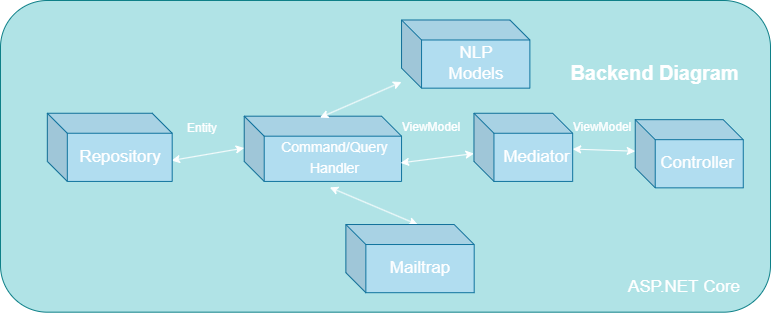
\includegraphics[width=150mm]{figs/backendDiagram.png}
	\caption{Diagrama modulului de backend}
	\label{fig:backendDiagram}
\end{figure}

Modulul de backend este, de fapt, serverul din arhitectura client-server. Acesta se ocupă de procesarea request-urilor venite de la utilizator folosind un mediator.\\
Problema pe care o rezolvă adăugarea unui mediator este decuplarea componentelor unui sistem. Acestea nu vor comunica în mod direct între ele, interacțiunea fiind mediată. Avantajul folosirii interacțiunii mijlocite 
constă în faptul că, dacă vor apărea modificări noi, componentele deja existente nu vor fi afectate. \\
Poate exista, într-adevăr, și un dezavantaj - poate ajunge destul de complex în funcție de cerințele sistemului, așa cum este menționat aici ~\cite{MediatorDisadvantage}.\\

Legătura dintre backend și baza de date se face în felul următor: în fișierul din modulul de backend există un fișier {\it appsettings.json} unde se declară un ConnectionString pentru conexiunea la baza de date (poate fi văzut în figura \ref{fig:connectionString}, creată utilizând~\cite{Carbon}). Acel string de conexiune conține numele
bazei de date și alte câteva atribute care permit conectarea, dar pot fi opționale. 

\begin{figure}[H]
	\centering
	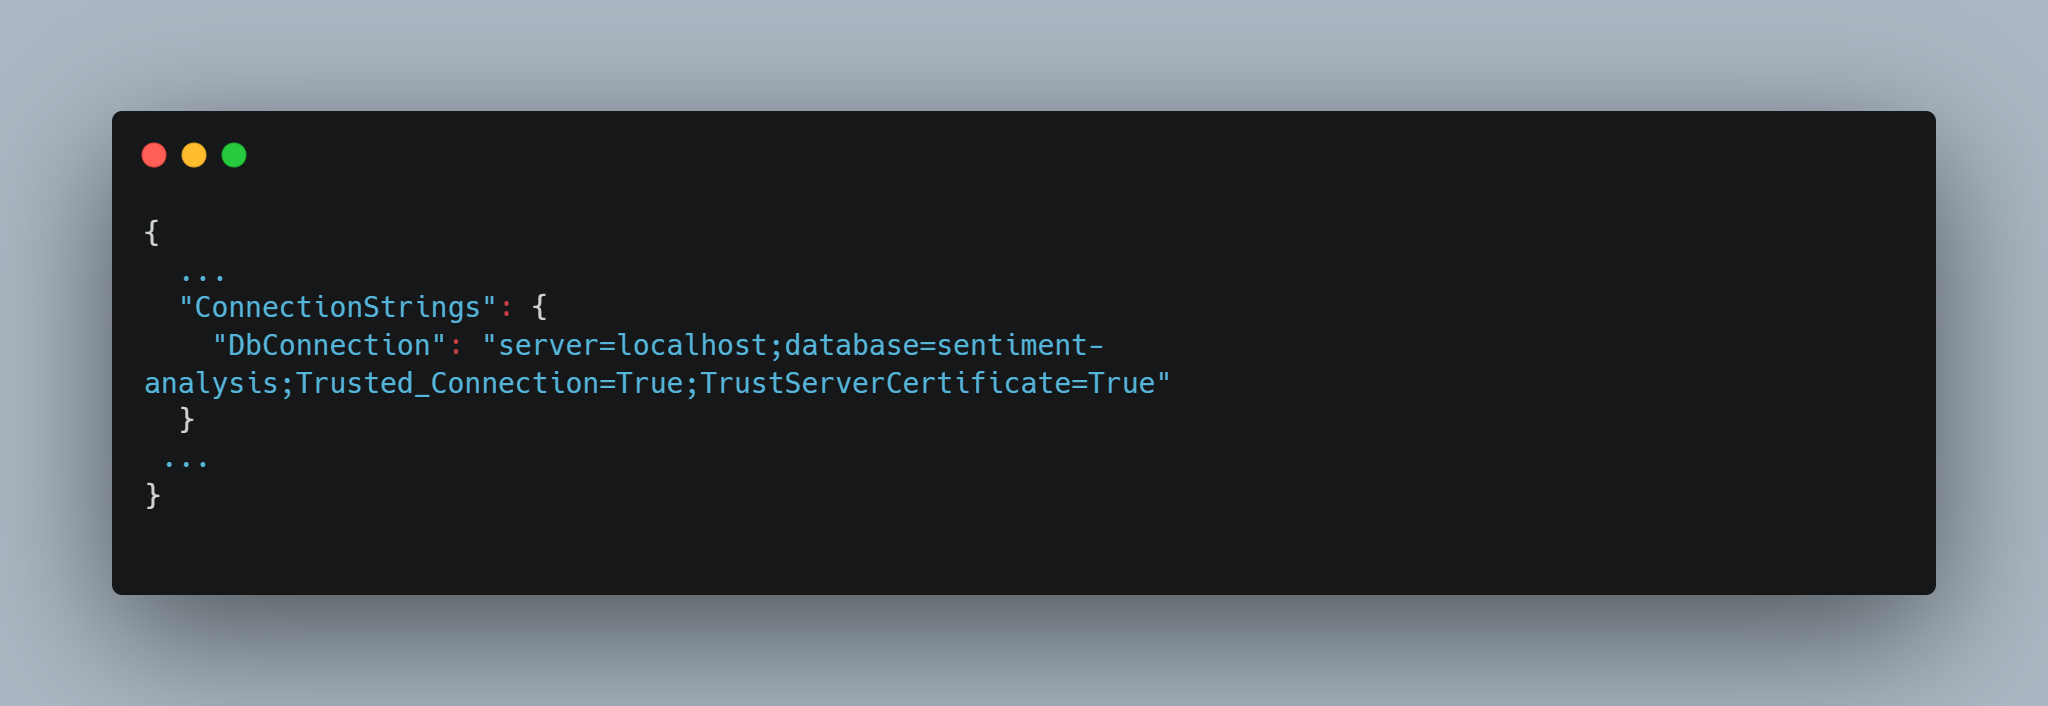
\includegraphics[width=150mm]{figs/connectionString.png}
	\caption{String de conectare backend cu baza de date}
	\label{fig:connectionString}
\end{figure}

\subsubsection{Repository}
În acest nivel se află legătura dintre aplicație și baza de date. Modelele create aici vor deveni entitați ale bazei de date.
Spre exemplu, clasa User cu atributele Id, FirstName, LastName, Username, Email, PasswordSalt, PasswordHash, va determina structura și atributele tabelei Users din baza de date, cea din urmă având toate atributele prezentate în clasă.

După crearea unui model, Entity Framework Core permite configurarea suplimentară a modelului, după cum poate fi văzut în figura \ref{fig:userEntityTypeConfiguration} și nu mai sunt necesare adnotări pentru atribute. În acest mod, a fost specificat că 
atributul de Id este cheie primară (implicit nu poate fi null), iar celelalte atribute FirstName, LastName, Username, Email, PasswordHash, PasswordSalt trebuie să fie diferite de null. 
\begin{figure}[H]
	\centering
	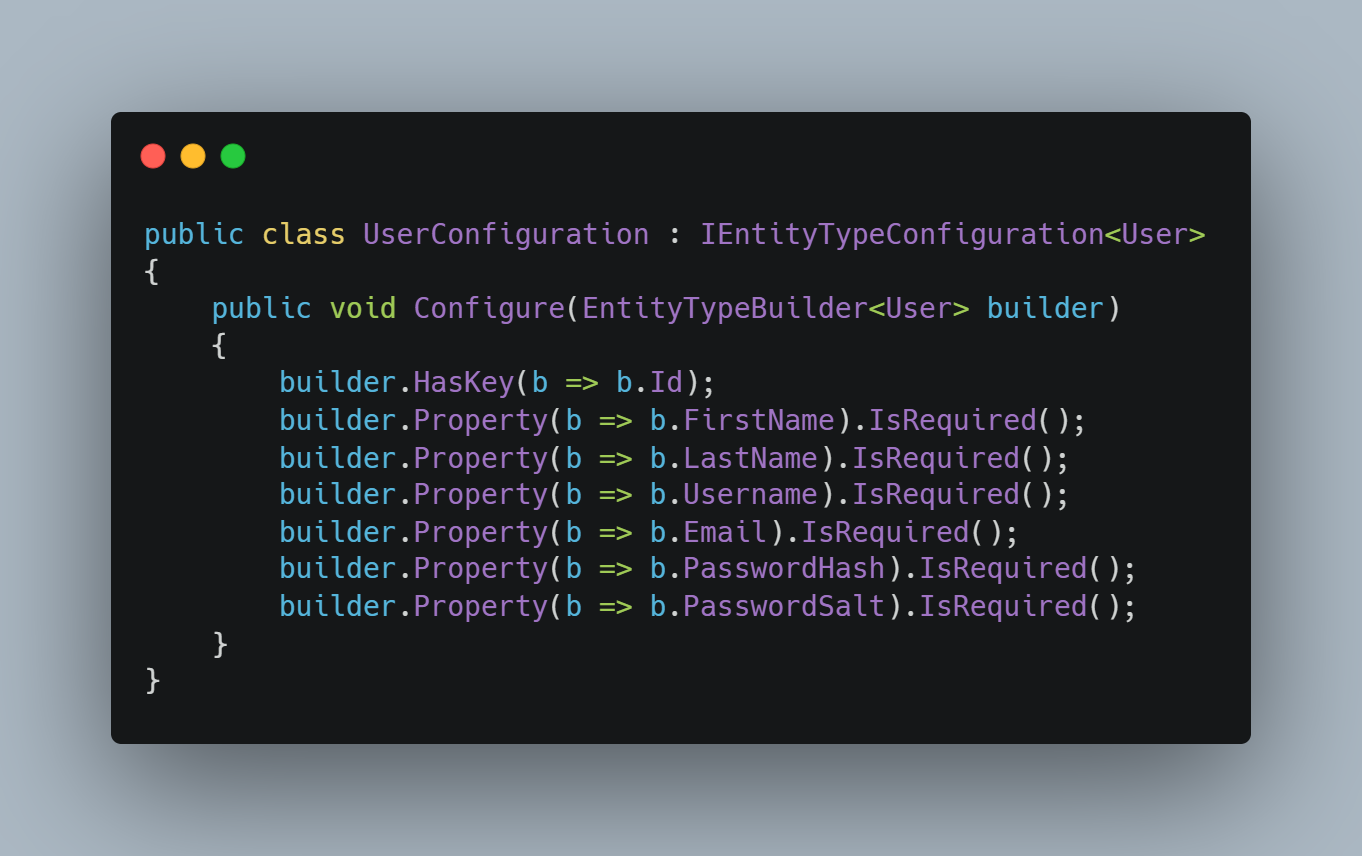
\includegraphics[width=100mm]{figs/userEntityTypeConfiguration.png}
	\caption{Configurare pentru modelul unui utilizator}
	\label{fig:userEntityTypeConfiguration}
\end{figure}

Aici se introduce conceptul de DbContext, care reprezintă o sesiune cu baza de date, când se pot face operații de tip stocare, interogare, actualizare și ștergere a elementelor din baza de date, creare de modele și maparea datelor.\\
DbContext este responsabil de deschiderea și gestionarea conexiunilor cu baza de date. \\
Pentru crearea unui model, DbContext îl construiește bazându-se pe configurarea dată și apoi este mapat. Pentru maparea datelor, rezultatele interogărilor sunt mapate la instanțe și entități definite de utilizator, cum sunt in figura \ref{fig:dbContext}.\\

Se adaugă conceptul de DbSet, prin care este posibilă aplicarea operațiilor de tip stocare, interogare, actualizare, ștergere pe acea entitate.\\
Clasele DbSet sunt proprietăți ale DbContextului și sunt mapate la baza de date care iau numele dat de utilizator.
DbSet este o implementare a patternului Repository, care înceară să adauge un layer între nivelul de acces la baza de date și nivelul de logică.

\begin{figure}[H]
	\centering
	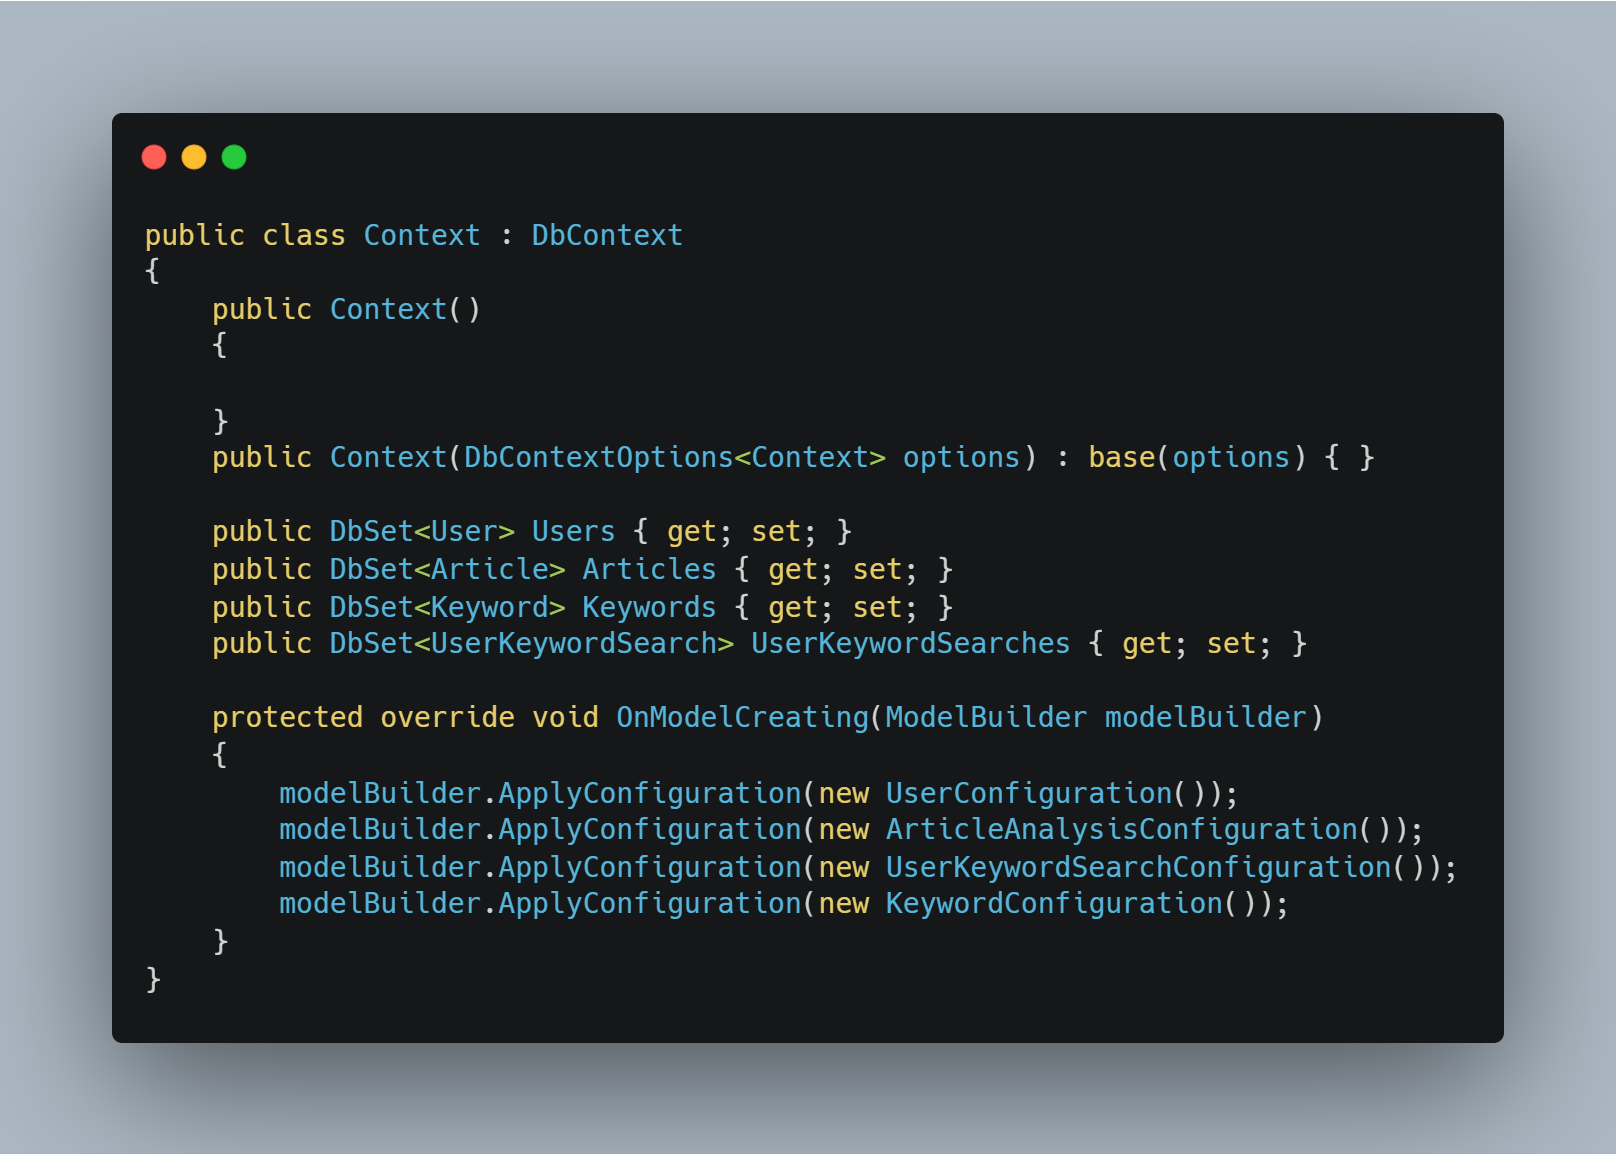
\includegraphics[width=150mm]{figs/dbContext.png}
	\caption{Configurare DbContext}
	\label{fig:dbContext}
\end{figure}

\subsubsection{Command/Query Handler}
Aici se află partea de logică și procesare a datelor din aplicație. Prin procesarea datelor înțelegem toate interacțiunile ce pot exista cu baza de date și din această cauză a fost introdus un pattern al cărui scop este de separare a operațiilor de citire și scriere în baza de date - CQRS sau Command and Query Responsibility Segregation. \\

Așadar, se face o separare în 2 modele, comenzi și interogări. Comenzile sunt, de fapt, operațiile ce presupun stocarea, actualizarea sau ștergerea din baza de date, iar interogările reprezintă citirile din baza de date. \\
În partea de comenzi, operațiile care se fac sunt următoarele, în funcție de clasă:
\begin{itemize}
	\setlength\itemsep{0.5em}
	\item User
	\begin{itemize}
		\setlength\itemsep{0.5em}
		\item AddUserCommand - care adaugă un utilizator nou, folosită pentru crearea unui cont nou
		\item EditUserCommand - care actualizează detaliile unui utilizator
		\item DeleteUserCommand - care șterge un utilizator
	\end{itemize}
	\item UserKeywordSearches
	\begin{itemize}
		\setlength\itemsep{0.5em}
		\item AddUserKeywordSearchCommand - care adaugă o nouă căutare ce cuprinde cuvântul cheie sau expresia identificată în textul analizat
	\end{itemize}
	\item Articles
	\begin{itemize}
		\setlength\itemsep{0.5em}
		\item AddArticleCommand - care adaugă un nou articol ce cuprinde toate rezultatele analizei efectuate pe un text financiar
		\item DeleteArticleCommand - care șterge un articol ce cuprinde toate rezultatele analizei efectuate pe un text financiar
	\end{itemize}
\end{itemize}
În partea de interogări, operațiile care se fac sunt următoarele, în funcție de clasă:
\begin{itemize}
	\setlength\itemsep{0.5em}
	\item User
	\begin{itemize}
		\setlength\itemsep{0.5em}
		\item GetUserDetailsQuery - care cere informațiile despre un anumit utilizator, într-un anumit format solicitat
		\item EditUserCommand - care actualizează detaliile unui utilizator
		\item DeleteUserCommand - care șterge un utilizator
	\end{itemize}
	\item UserKeywordSearches
	\begin{itemize}
		\setlength\itemsep{0.5em}
		\item GetKeywordStatisticsQuery - care interoghează baza de date și trimite înregistrările găsite pentru un anumit cuvânt cheie sau expresie într-o perioadă selectată
		\item GetSearchNumberOfOccurrencesQuery - care interoghează baza de date și trimite înregistrările pe zile pentru itemii (cuvinte cheie sau expresii) găsite în perioada selectată de timp
		\item FilterSearchesByPeriodCommand - care interoghează baza de date și trimite înregistrările găsite într-o perioadă selectată pentru cele mai populare 10 subiecte
	\end{itemize}
	\item Articles
	\begin{itemize}
		\setlength\itemsep{0.5em}
		\item GetArticlesQuery - care interoghează baza de date și trimite înregistrările găsite pentru pentru un anumit input, adică toate articolele salvate ale unui utilizator
		\item GetUserArticleQuery - care interoghează baza de date și trimite informații despre articolul selectat pentru ca utilizatorul să poată revedea analiza detaliată
	\end{itemize}
	\item TextAnalysis
	\begin{itemize}
		\setlength\itemsep{0.5em}
		\item GetSentimentScoreQuery - care realizează inferența modului de analiză de sentiment având drept input textul introdus de utilizator
		\item GetTextSummaryQuery -  care realizează inferența modului de sumarizare a textului având drept input textul introdus de utilizator
		\item GetKeyphrasesQuery - care realizează inferența modului de extragere a cuvintelor cheie sau expresiilor având drept input textul introdus de utilizator
	\end{itemize}
\end{itemize}
\paragraph{Model de comandă}
\begin{figure}[H]
	\centering
	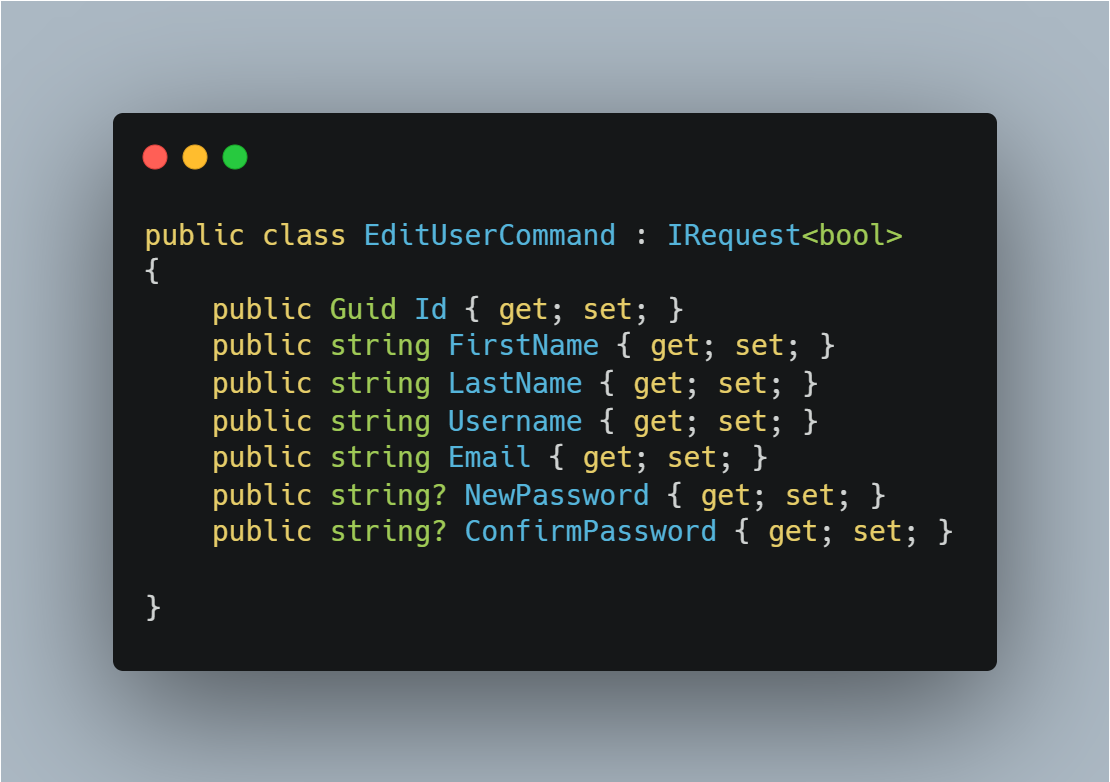
\includegraphics[width=100mm]{figs/editUserCommand.png}
	\caption{Comandă de editare utilizator}
	\label{fig:editUserCommand}
\end{figure}
Interfața IRequest acceptă tipul obiectului pe care Handlerul ar trebui să îl returneze, în acest caz, o valoare true sau false.
Un handler pentru această comandă este următorul, în figura \ref{fig:editUserCommandHandler}.
\begin{figure}[H]
	\centering
	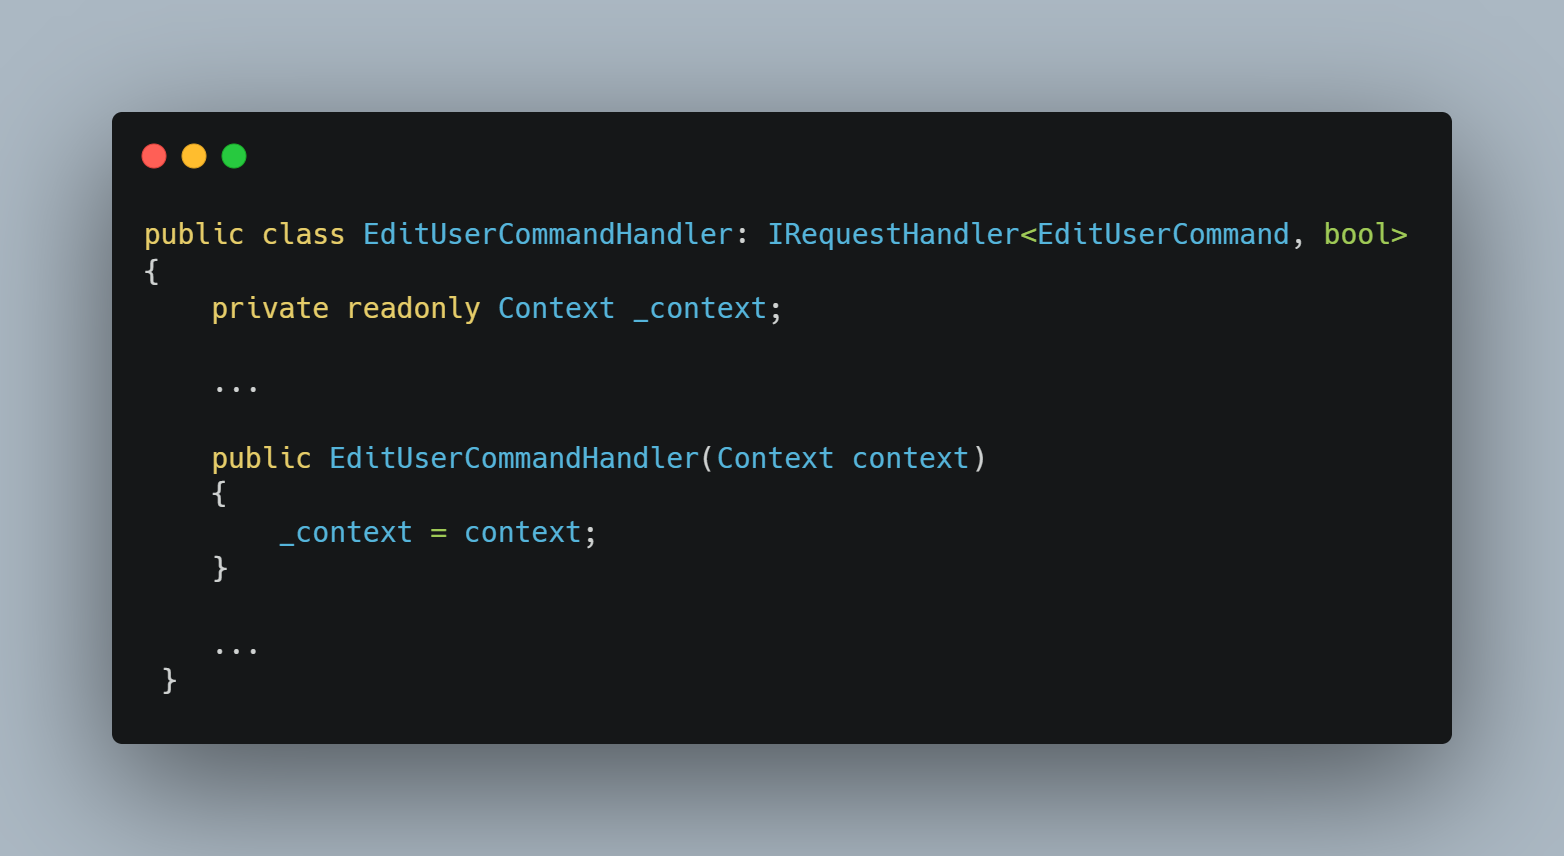
\includegraphics[width=150mm]{figs/editUserCommandHandler.png}
	\caption{Handler pentru comanda de editare utilizator}
	\label{fig:editUserCommandHandler}
\end{figure}
IRequestHandlerul acceptă 2 tipuri de parametri, după cum e specificat și aici~\cite{IRequestHandler}: requestul la care trebuie să răspundă și tipul care trebuie returnat.
\paragraph{Model de query}
În figura \ref{fig:getUserArticleQuery} este un query care solicită ca răspuns un ArticleViewModel (un model pentru vizualizare a unui articol salvat de utilizator), atunci când primește ca identificatori un UserId și un ArticleId.
Handlerul poate fi văzut în figura \ref{fig:getUserArticleQueryHandler}.
\begin{figure}[H]
	\centering
	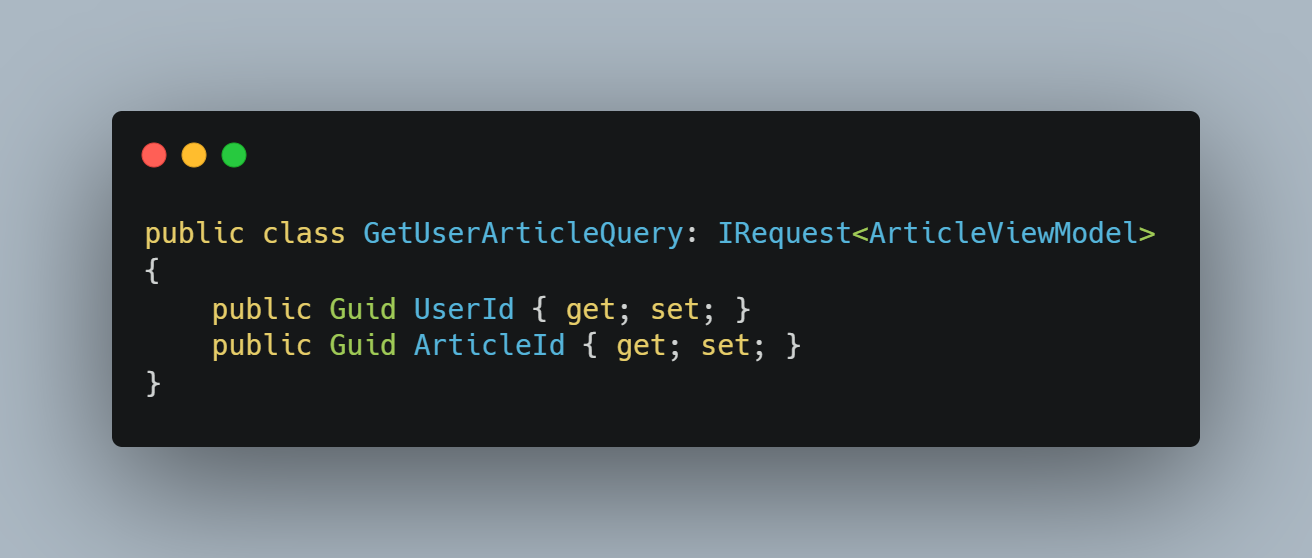
\includegraphics[width=100mm]{figs/getUserArticleQuery.png}
	\caption{Query de citire a informațiilor despre un articol salvat de utilizator}
	\label{fig:getUserArticleQuery}
\end{figure}

\begin{figure}[H]
	\centering
	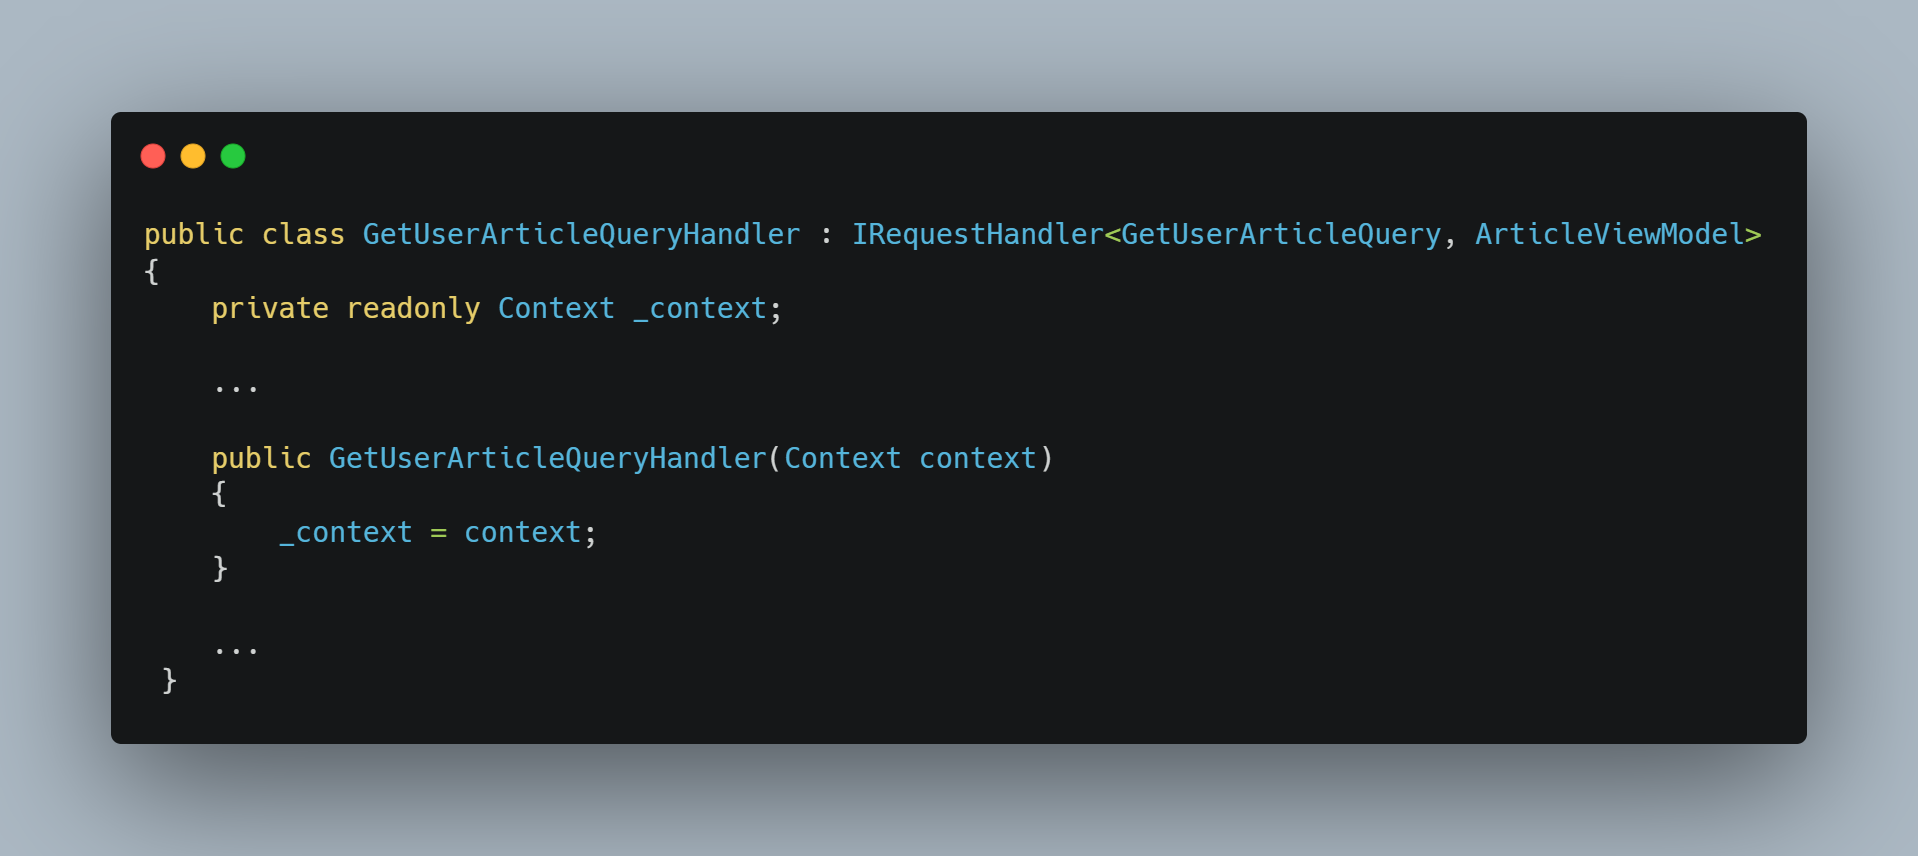
\includegraphics[width=100mm]{figs/getUserArticleQueryHandler.png}
	\caption{Handler al unui query de citire a informațiilor despre un articol salvat de utilizator}
	\label{fig:getUserArticleQueryHandler}
\end{figure}

\begin{figure}[H]
	\centering
	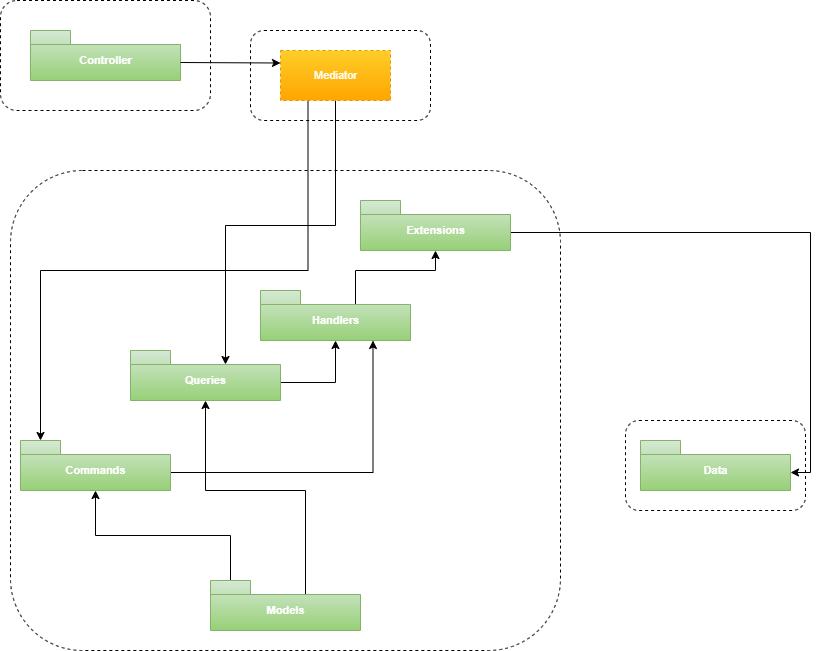
\includegraphics[width=150mm, height=100mm]{figs/packageBE.png}
	\caption{Diagrama pachetelor din modulul de backend}
	\label{fig:packageBE}
\end{figure}

După cum se poate vedea, handlerul este asemănător cu handler-ul comenzii de mai sus, diferența o face rezultatul trimis și metodele de validare din clase.
Tot în partea de logică a aplicației, sunt câteva handlere cu funcționalitate mai specială. 
\paragraph{Adăugare user nou}
\ \\
La crearea unui cont nou, în comandă sunt scrise toate informațiile necesare. De aici, câmpul de email mai este folosit și în trimiterea unui mail de confirmare a înregistrării. 
Pentru acest lucru am folosit Mailtrap, un server SMTP care ajută la testarea acestei funcționalități. 
Handlerul pentru această funcționalitate este în figura \ref{fig:sendRegistrationMail}.
\begin{figure}[H]
	\centering
	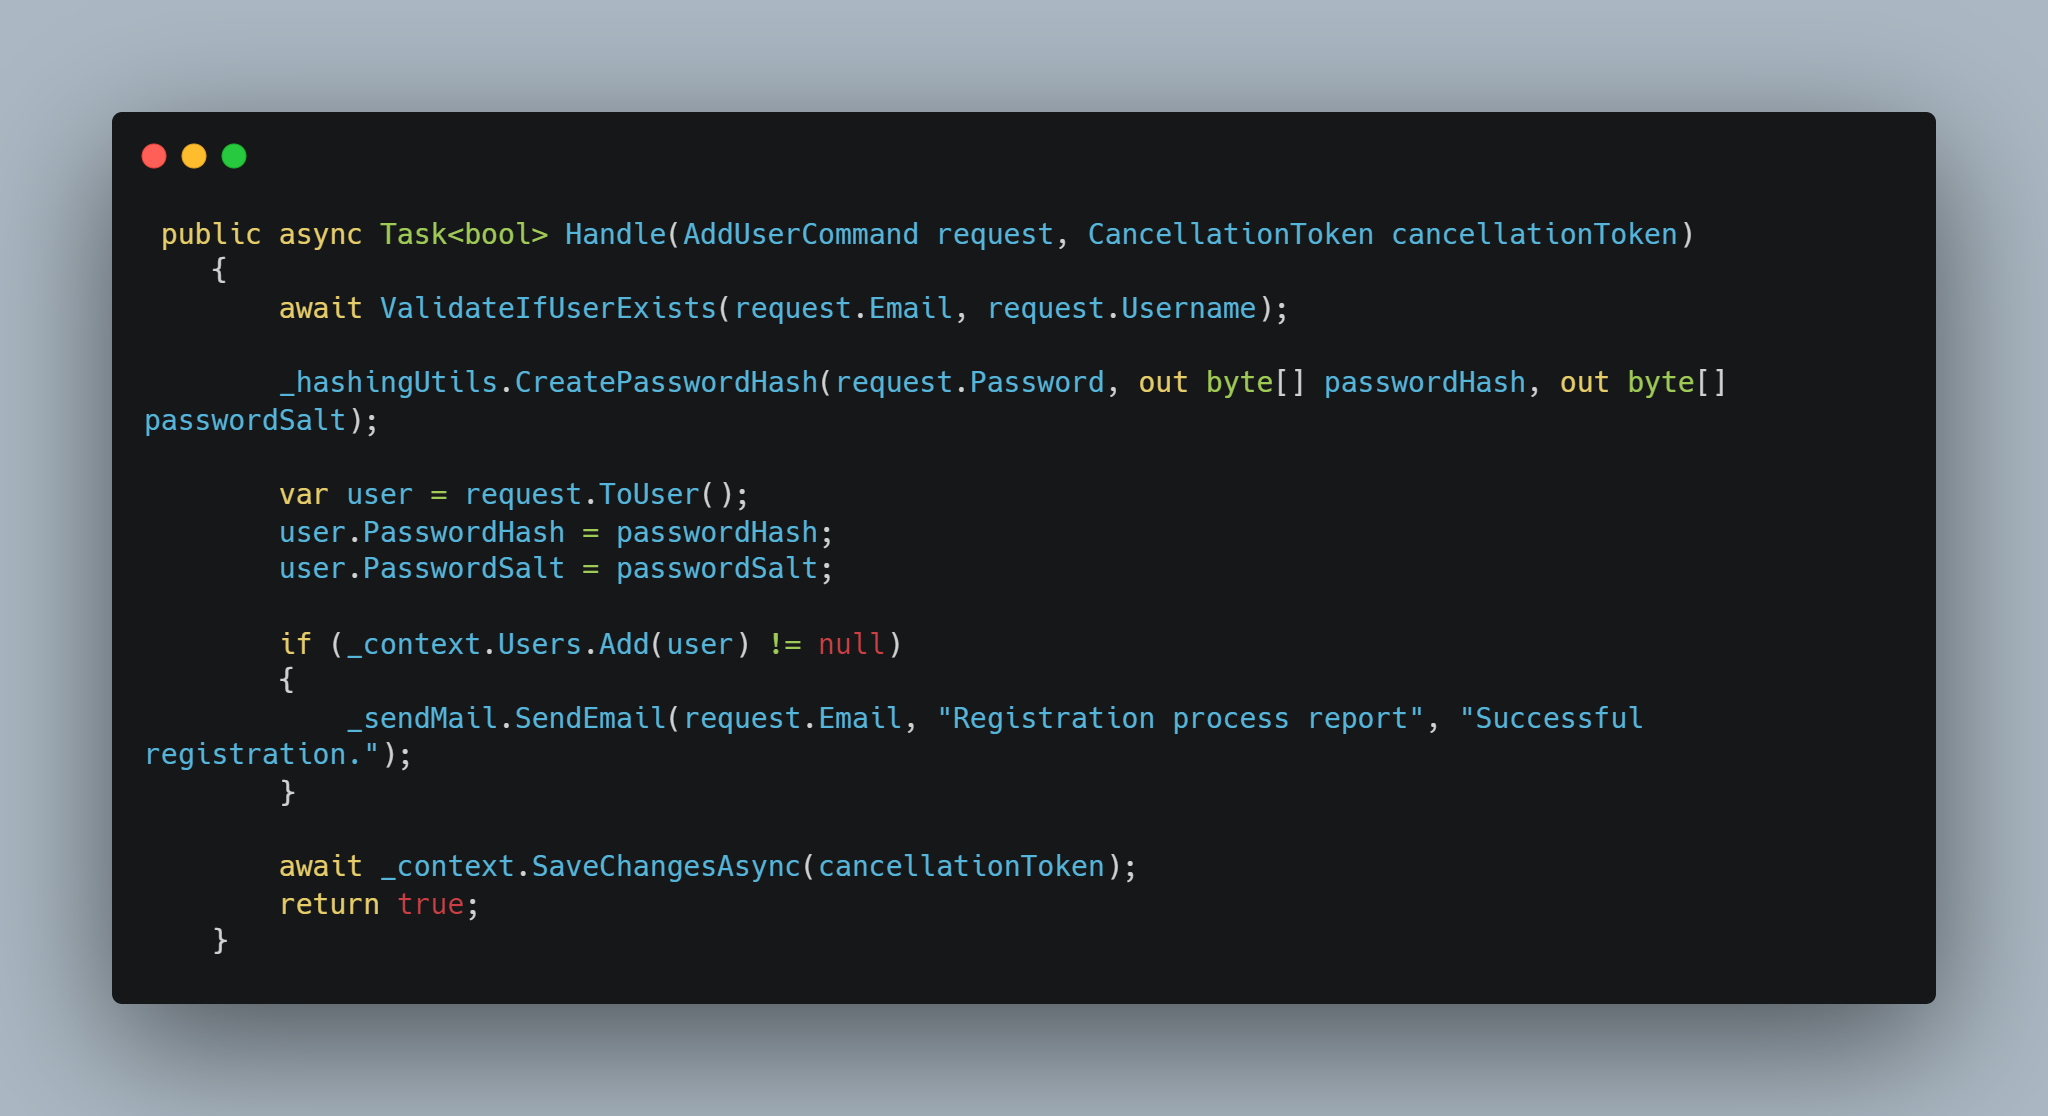
\includegraphics[width=100mm]{figs/sendRegistrationMail.png}
	\caption{Handler al unui query de citire a informațiilor despre un articol salvat de utilizator}
	\label{fig:sendRegistrationMail}
\end{figure}
Mai întâi se verifică dacă mai există alt utilizator cu același email sau nume de utilizator. În cazul în care există, va fi aruncată o excepție, altfel se continuă cu crearea unei parole criptate, se adaugă noul utilizator în baza de date și se trimite un email. 
Un exemplu de email este în figura \ref{fig:registrationReport}.
\begin{figure}[H]
	\centering
	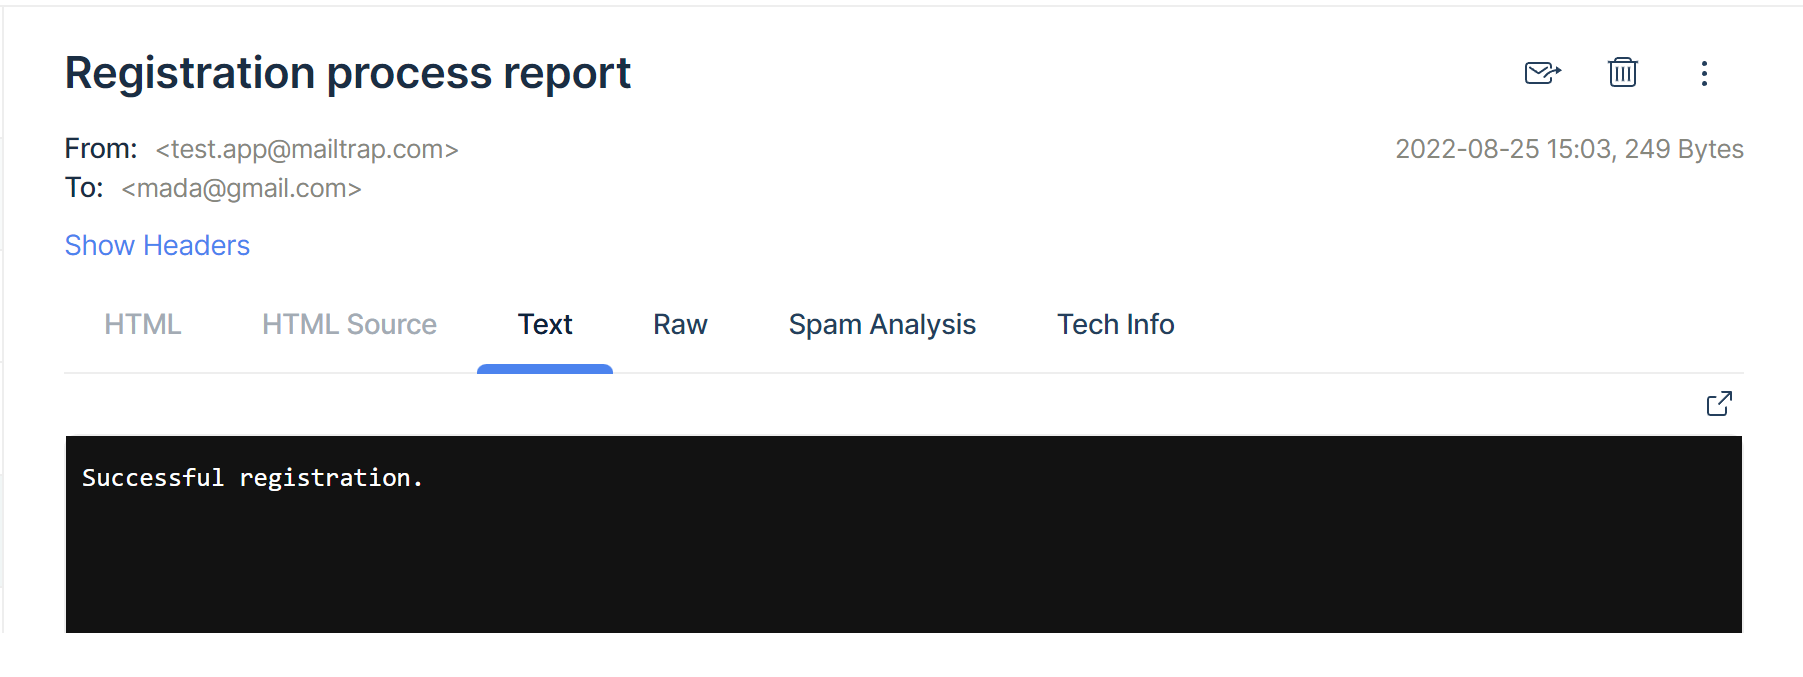
\includegraphics[width=100mm]{figs/registrationReport.png}
	\caption{Email de confirmare a procesului de creare de cont cu succes}
	\label{fig:registrationReport}
\end{figure}


Handlerele care se ocupă de analiza sentimentelor dintr-un text financiar, sumarizarea textului și extragerea cuvintelor cheie se află tot aici. Acestea folosesc un serviciu pentru a apela metodele specifice,exemplu în figururile \ref{fig:getKeyphrasesHelper} și \ref{fig:huggingFaceHelper} .
\begin{figure}[ht]
	\centering
	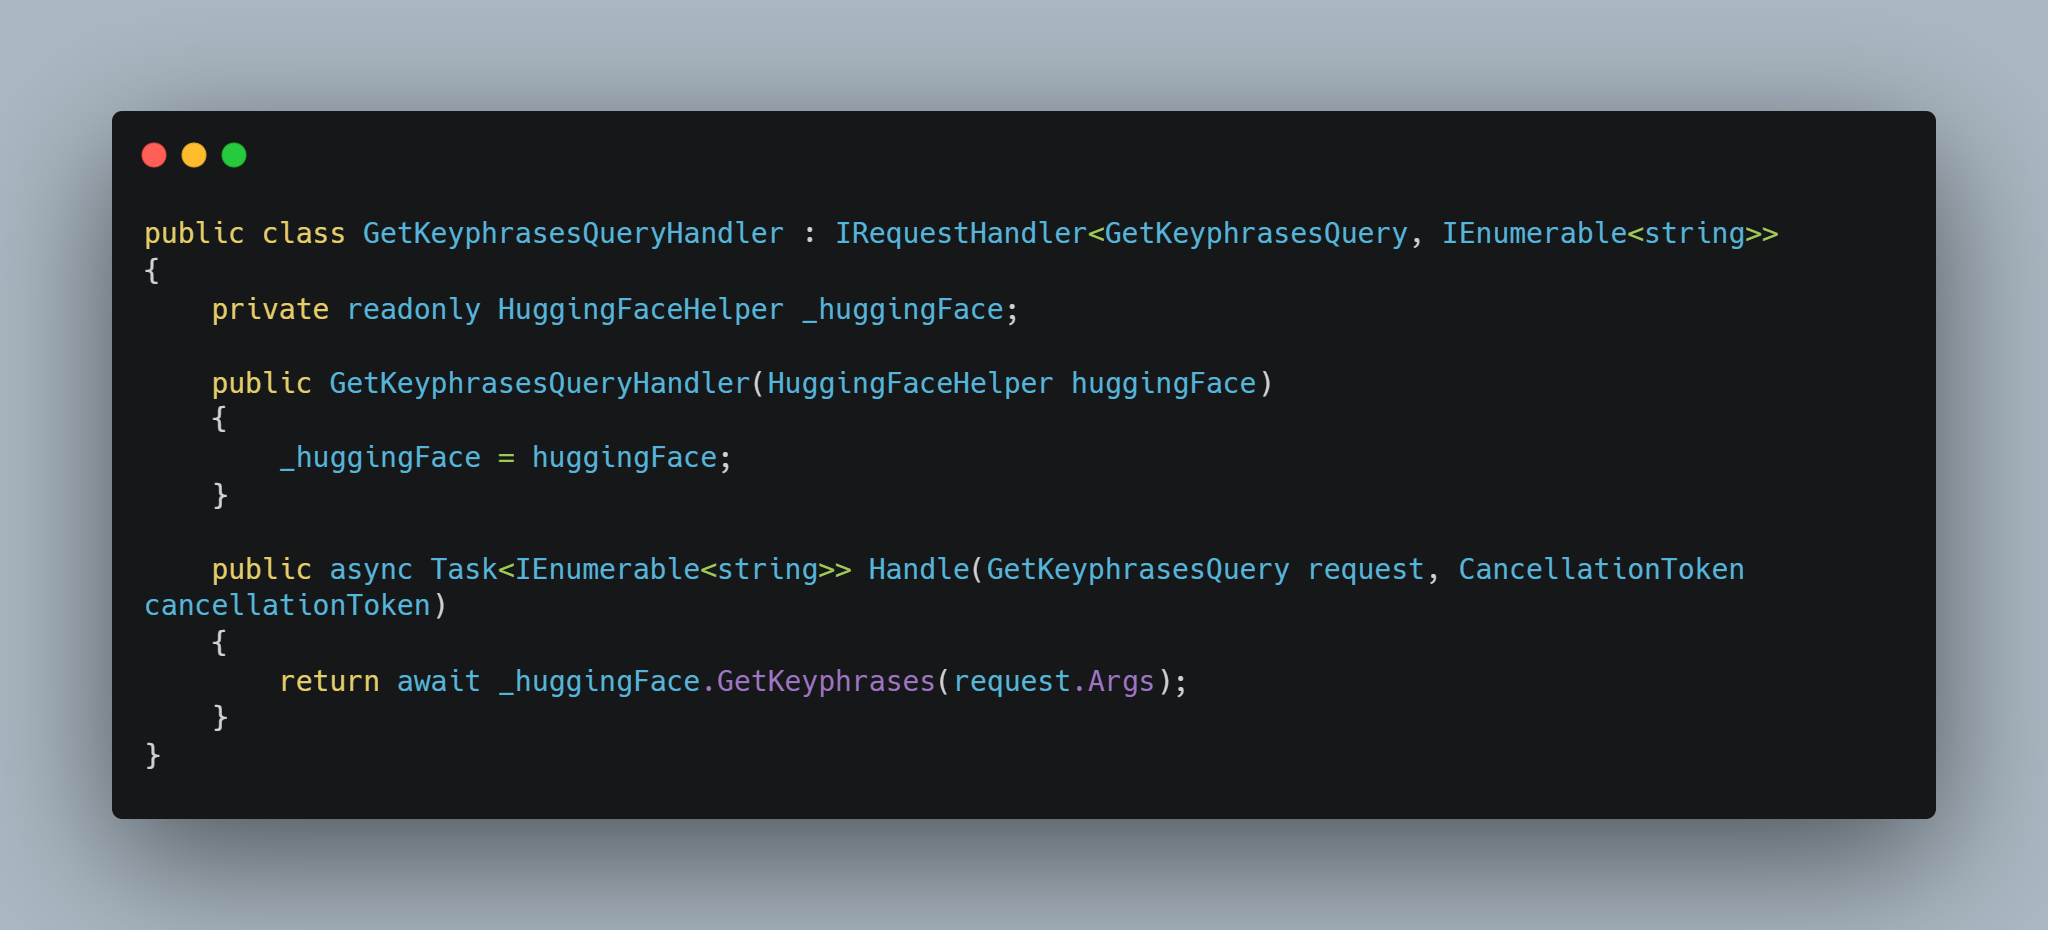
\includegraphics[width=150mm]{figs/getKeyphrasesHelper.png}
	\caption{Handler pentru extragerea cuvintelor cheie}
	\label{fig:getKeyphrasesHelper}
\end{figure}

Handlerul apelează metoda GetKeyphrases, având ca parametru textul introdus de utilizator. \\ HuggingFaceHelper este utilizat ca un serviciu și este posibilă apelarea metodelor din clasă. \\
Metoda menționată apelează altă metodă, CallModel, cu un URL pentru modelul care extrage cuvintele cheie și inputul utilizatorului. În această metodă, se creează un body în format JSON pentru un request de tip POST,
se trimite, apoi se așteaptă răspunsul. \\ 

Dacă răspunsul nu conține mesaj de eroare, acesta este transmis spre client, altfel se face o extra-validare pentru a detecta dacă eroarea primită este o eroare din cauza încărcării modelului, iar în cazul care este,
metoda se va apela recursiv pentru a porni modelul și a primi rezultatul așteptat, după ce vor mai fi efectuate câteva parsări pentru formatul corect al acestuia. 

\begin{figure}[ht]
	\centering
	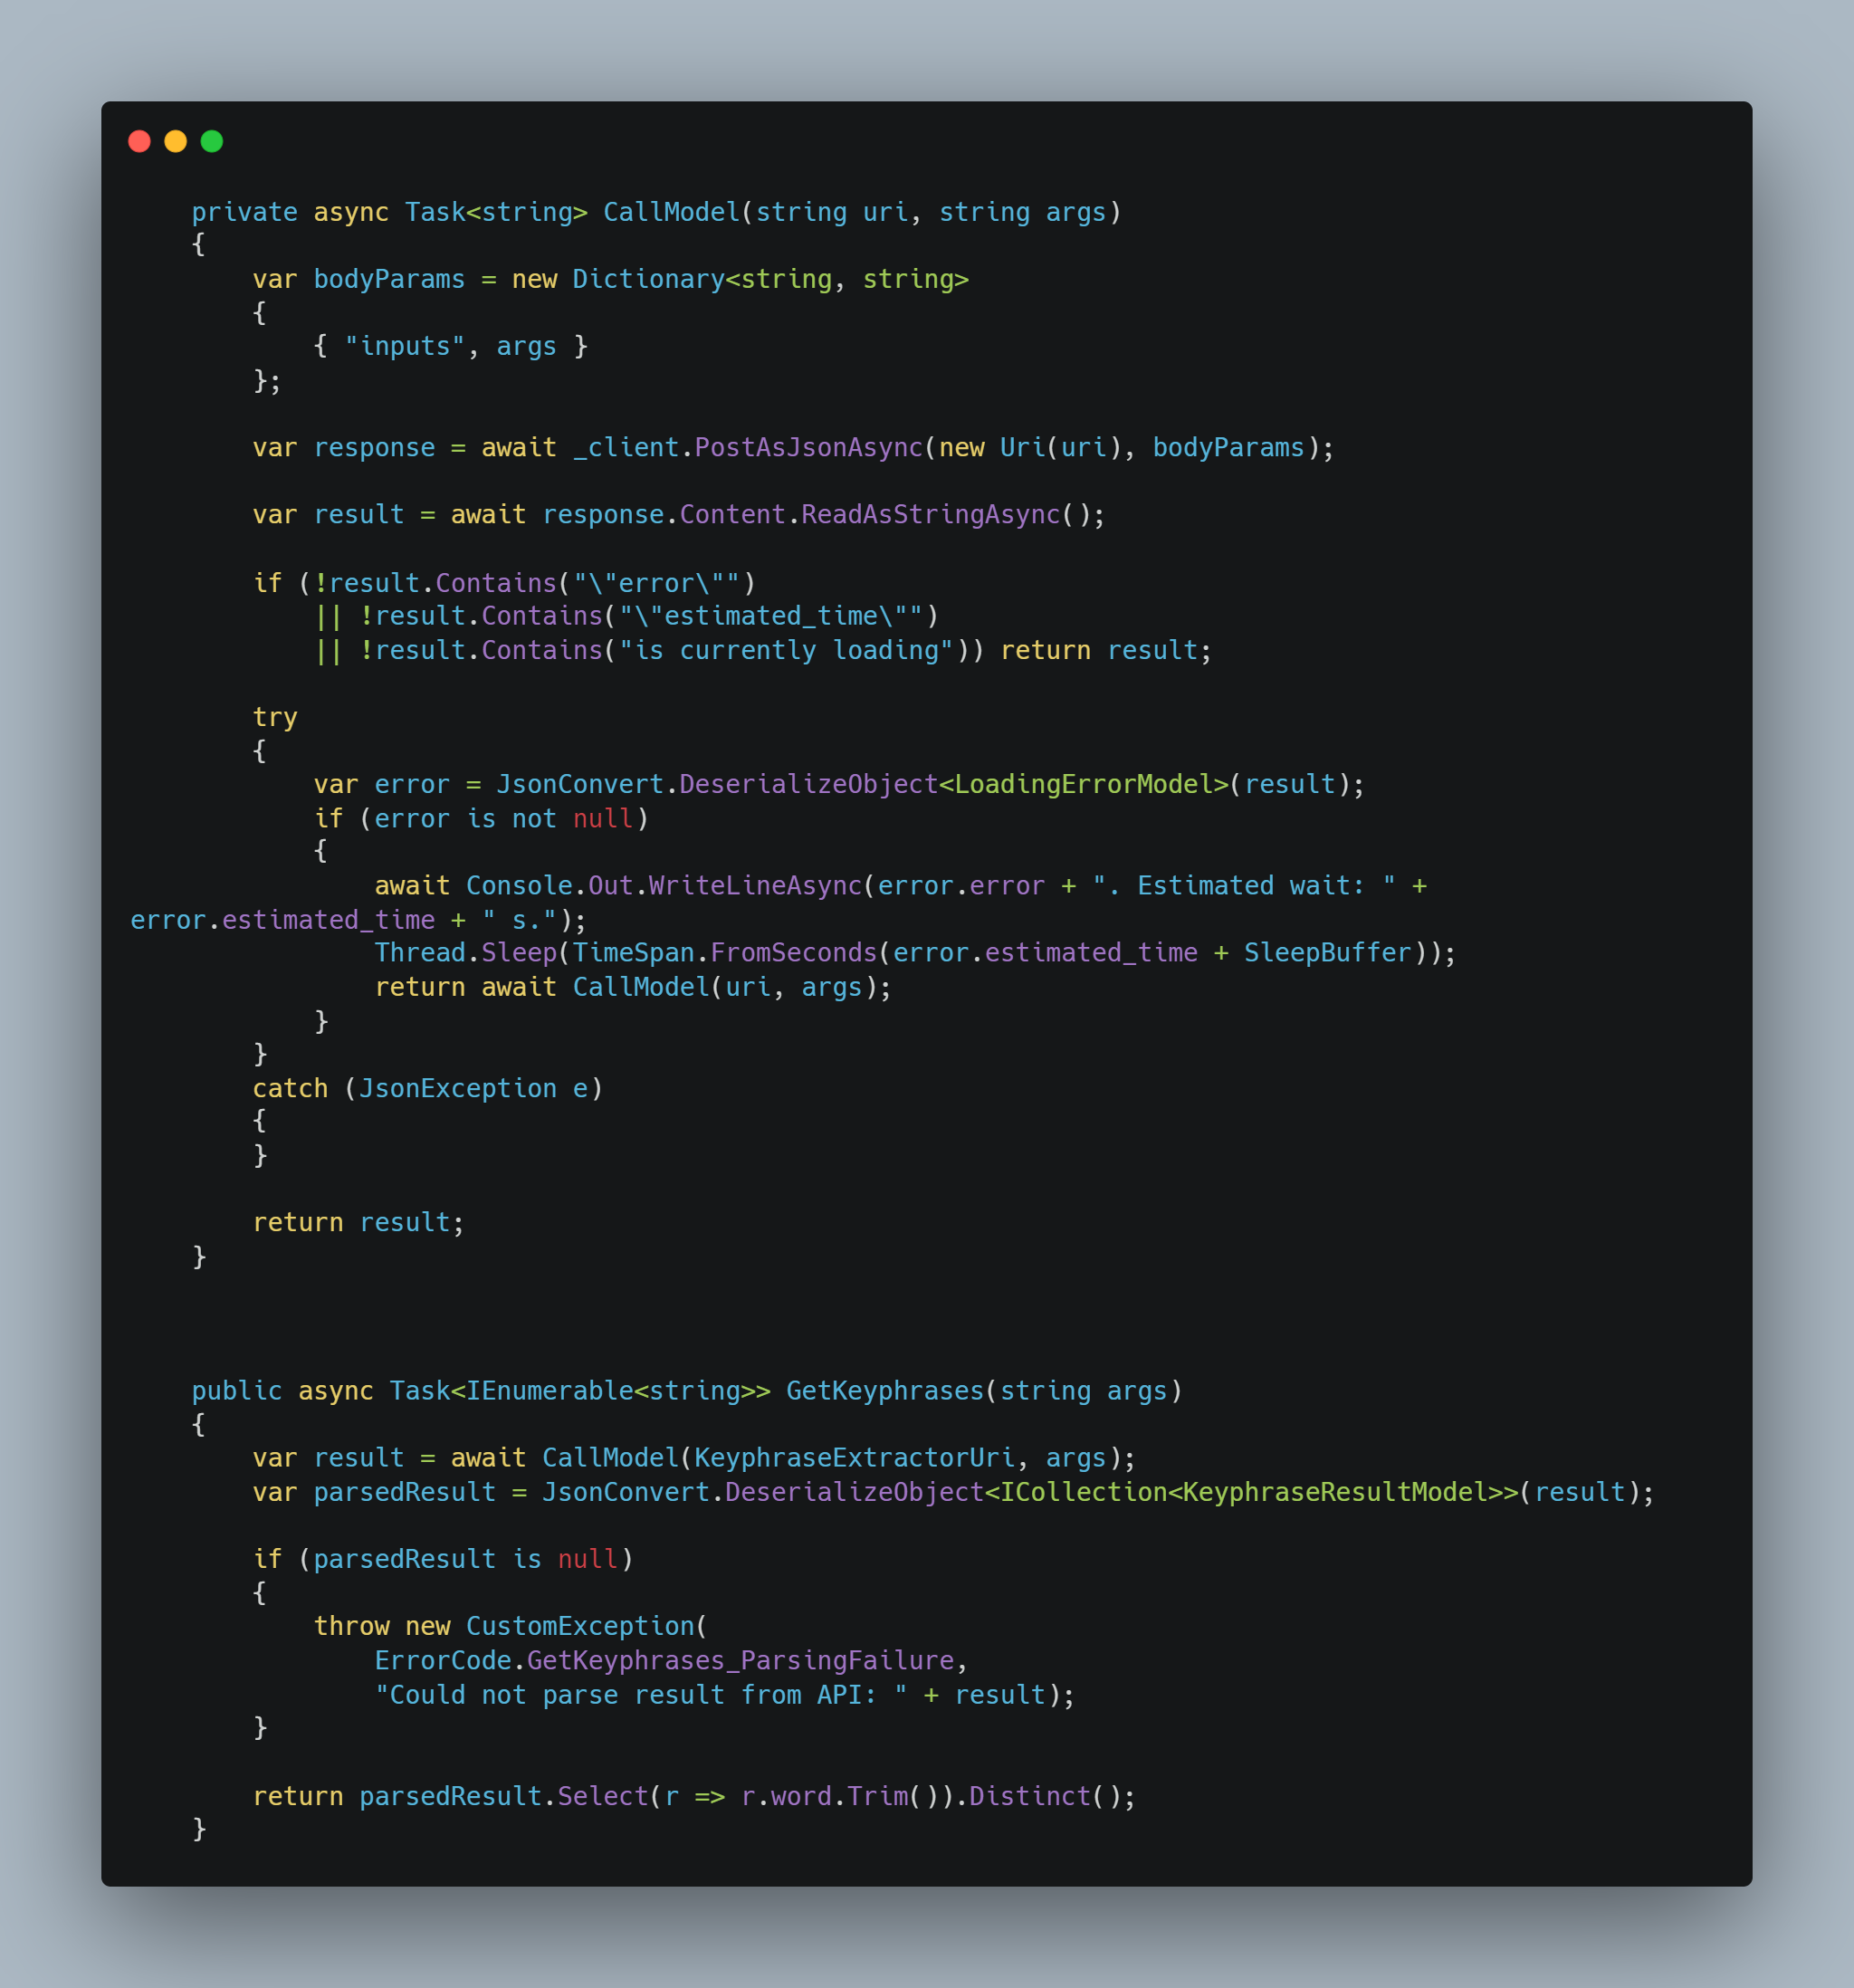
\includegraphics[width=150mm]{figs/huggingFaceHelper.png}
	\caption{Metode pentru a accesa funcționalitățile modelului NLP}
	\label{fig:huggingFaceHelper}
\end{figure}

Pentru cazurile în care metodele de validare aruncă excepții, pentru claritate cât mai mare a fluxului, excepțiile au fost customizate cu scopul de a fi transmise în format JSON în frontend și pentru a ajuta utilizatorul.
\begin{figure}[H]
	\centering
	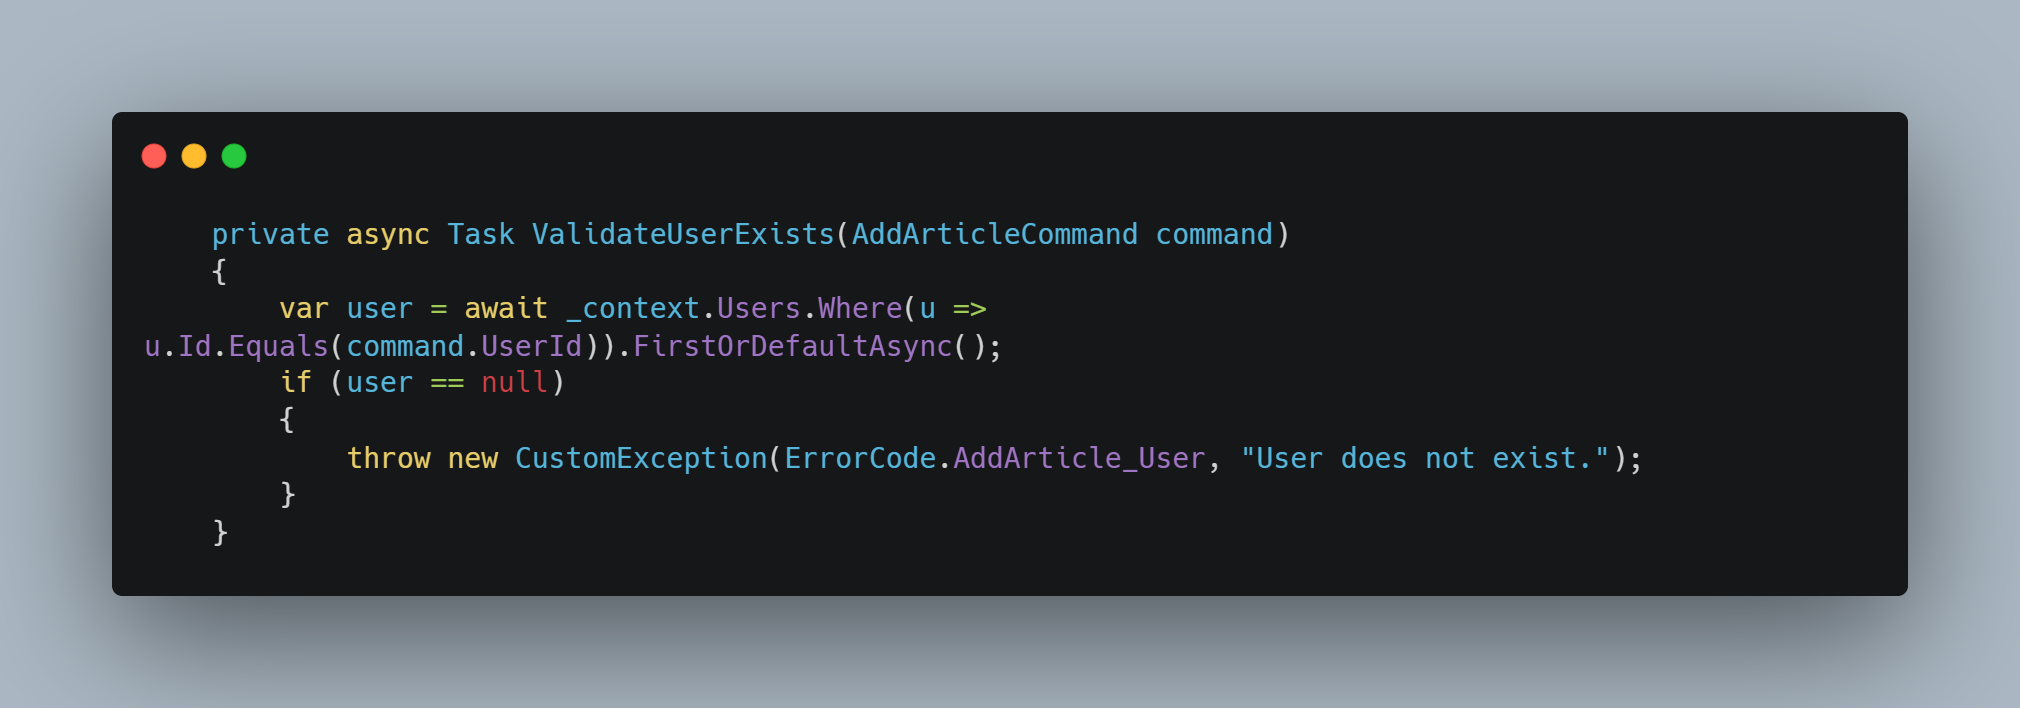
\includegraphics[width=150mm]{figs/customException.png}
	\caption{Exemplu validare care aruncă o excepție customizată}
	\label{fig:customException}
\end{figure}

Metoda din figura \ref{fig:customException} este folosită pentru validarea existenței unui utilizator al cărui Id corespunde cu cel din request.  \\ 
Dacă nu a fost găsit un utilizator și variabila este nulă, atunci o să se arunce o excepție cu mesajul din figură și un status customizat.

\subsubsection{Controllers}
Aici este nivelul în care modulul de frontend, clientul, interacționează cu modulul de backend, serverul, prin intermediul endpointurilor definite.\\
Un endpoint este, de fapt, un canal de comunicare, care include URL-ul spre o resursă.\\

Controllerele declarate sunt: UserController, ArticleController, UserKeywordsSearcheController, TextAnalysisController.\\
UserController conține endpoint-uri pentru adăugarea unui utilizator nou, logarea în aplicație, afișarea informațiilor unui utilizator, cât și editarea acestora. \\
Diagrama de secvență pentru procesul de logare în aplicație poate fi văzut în figura \ref{fig:sequnce}.
UserKeywordsSearcheController conține endpointuri pentru citirea căutărilor în funcție de anumite condiții. \\
TextAnalysisController conține endpointuri pentru extragerea cuvintelor cheie, sumarizarea textului și analiza sentimentelor pe text financiar.\\

Tot aici sunt declarate și tipul requesturilor: POST pentru adăugare, DELETE pentru ștergere, PUT pentru update, etc., după cum se poate vedea în figura \ref{fig:controllerExample}.
Mediatorul este adăugat pentru a gestiona (în handlere) requesturile, în funcție de tipul acestora: query pentru citiri din baza de date și commands pentru stocări sau actualizări ale bazei de date.

\begin{figure}[H]
	\centering
	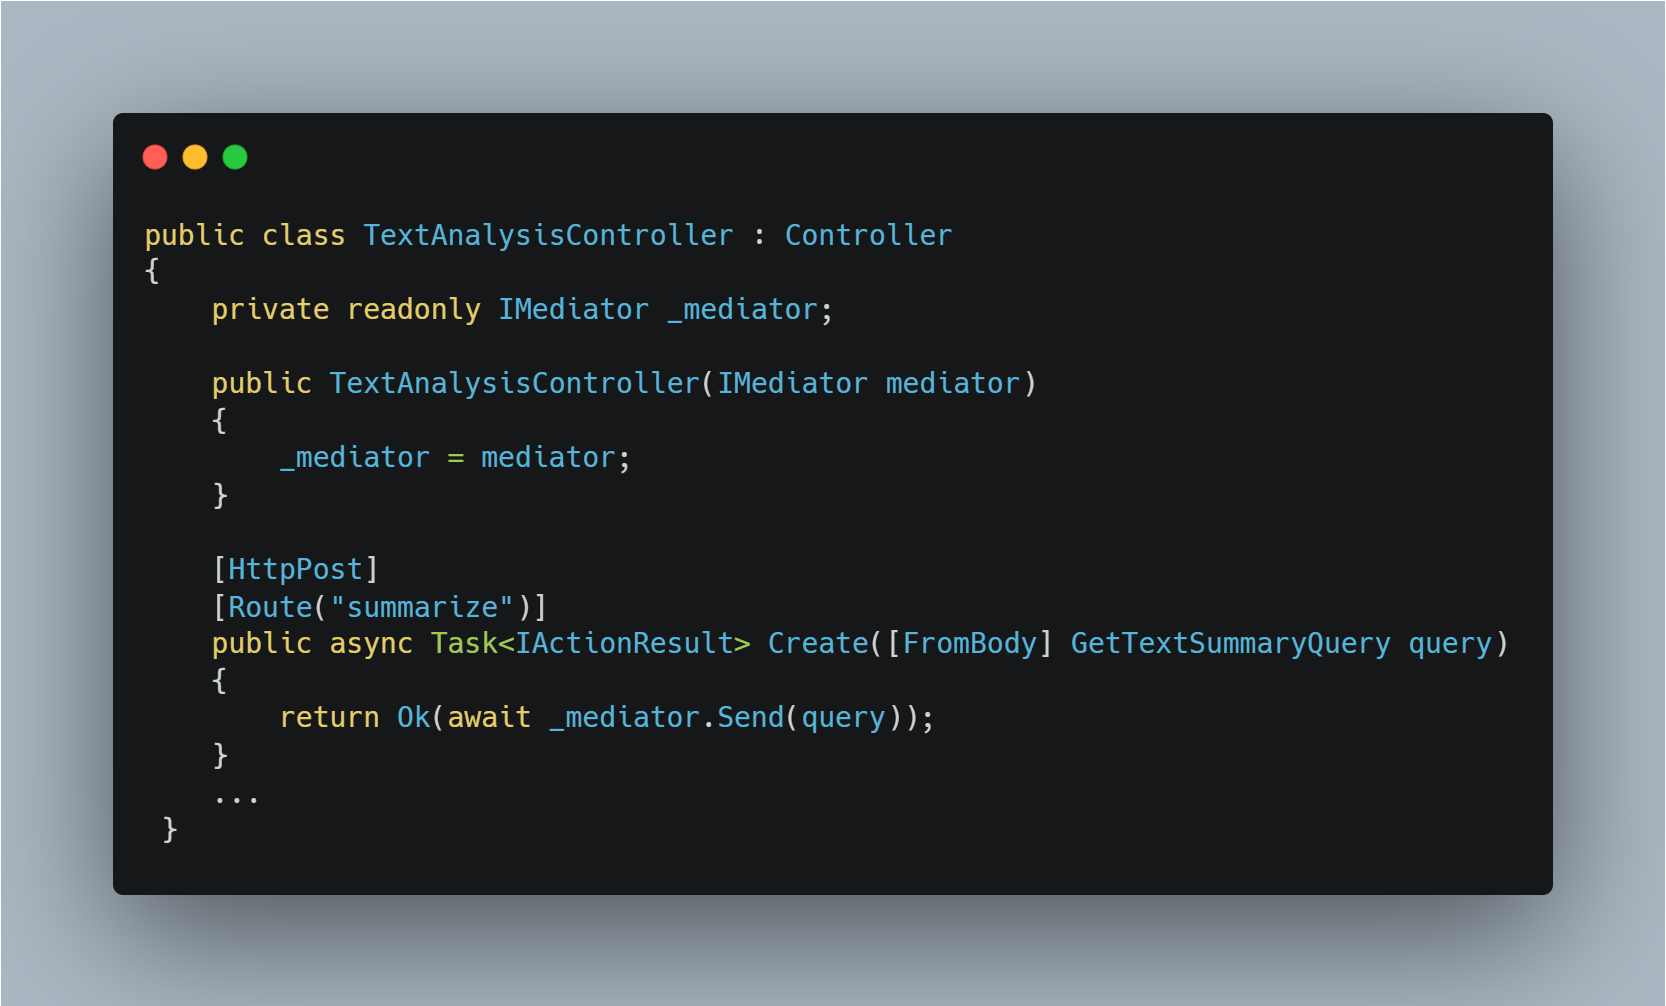
\includegraphics[width=150mm]{figs/controllerExample.png}
	\caption{Exemplu de controller cu Mediator}
	\label{fig:controllerExample}
\end{figure}

\section{Structura modulului de frontend}
În figura \ref{fig:frontendDiagram} este reprezentată diagrama modulului de backend.
\begin{figure}[H]
	\centering
	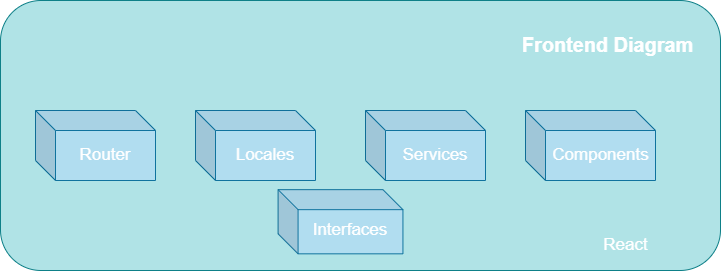
\includegraphics[width=150mm]{figs/frontendDiagram.png}
	\caption{Diagrama modulului de frontend}
	\label{fig:frontendDiagram}
\end{figure}

Diagrama pachetelor din acest modul poate fi văzută în figura \ref{fig:packageFE}.
\begin{figure}[h]
	\centering
	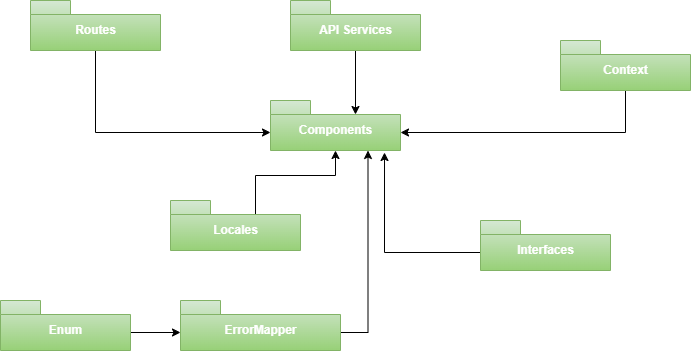
\includegraphics[width=150mm]{figs/packageFE.png}
	\caption{Diagrama pachetelor din modulul de frontend}
	\label{fig:packageFE}
\end{figure}

\subsubsection{Routes}

În modulul de frontend, componenta de Router se ocupă de rutare. \\ În general, o rută randează o pagină pentru un anumit URL.
În aplicație, pentru securitatea utilizatorului, au fost create rute publice și private. \\

Rutele publice reprezintă rutele pe care utilizatorul le poate accesa atunci când nu este autentificat, adică poate accesa paginile de Creare cont nou și de Logare în aplicație.\\

Pentru un utilizator neautentificat, orice încercare de a modifica forțat URL-ul și a accesa o rută privată, se rezumă la o redirecționare la o pagină cu rută publică.
Pentru rutele private, utilizatorul trebuie să aibă un cont creat și să fie logat. 
Pentru un utilizator autentificat, orice încercare de a modifica forțat URL-ul și accesa o rută publică, se rezumă la o redirecționare la pagina de Dashboard.\\

Pentru a putea gestiona global starea și pentru a obține statusul utilizatorului, dacă acesta este logat sau nu, se folosește un Context \ref{fig:reactContext}~\cite{ReactContext}.
\begin{figure}[h]
	\centering
	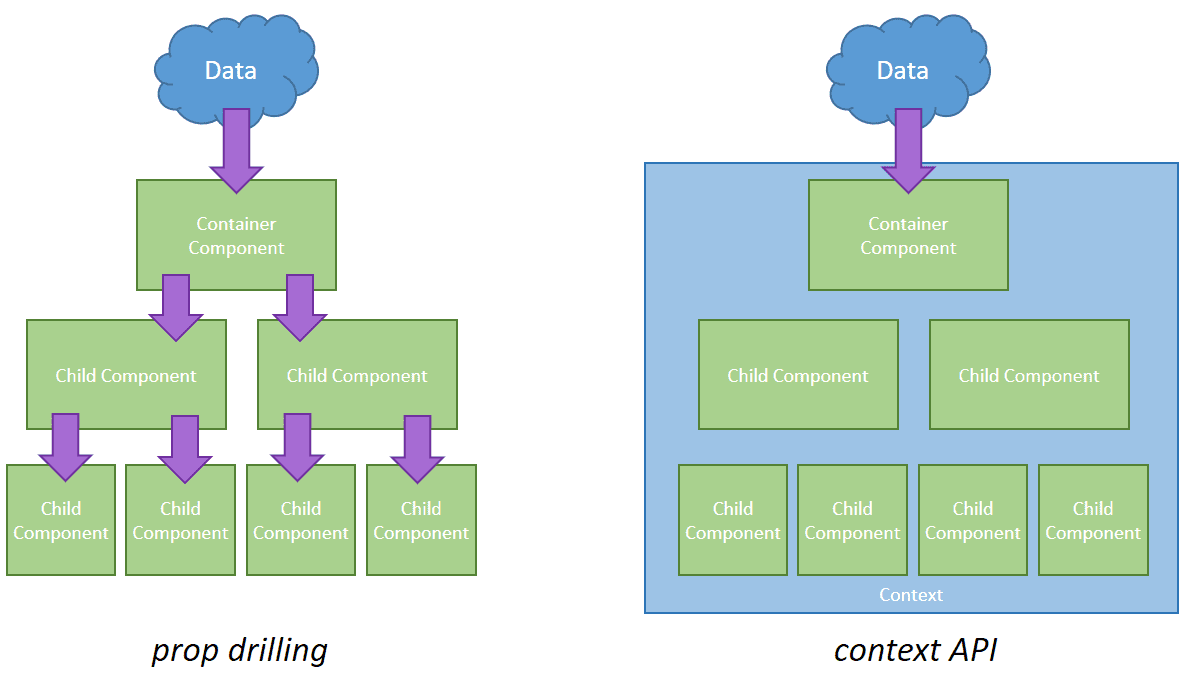
\includegraphics[width=150mm]{figs/reactContext.png}
	\caption{Contextul în React}
	\label{fig:reactContext}
\end{figure}

\subsubsection{Locales}
Internaționalizarea este implementarea unei aplicații astfel încât aceasta să fie disponibilă pentru utilizatori, indiferent de regiune.\\
Acest obiectiv a fost atins folosind i18n. Au fost create traduceri pentru toate textele din aplicație, fiind disponibile atunci când utilizatorul folosește switch-ul de limbă. 
Preferința utilizatorului va rămâne salvată, astfel încât atunci când va închide browserul și va reveni, va găsi aplicația în aceeași limbă.
\\

În fișierul index.ts din figura \ref{fig:i18nInstance}, trebuie asigurat faptul că librăria i18n este instalată și importurile sunt făcute pentru a beneficia de funționalitate.\\
Cu ajutorul funcției {\it use(...)} se pasează pluginul de i18n, apoi este inițializat cu resursele, care sunt fișierele de traduceri. În această aplicație, traducerile sunt pentru limba Engleză și limba Română.\\

{\it lng} este limba de început, dacă în localStorage există valoare pentru atributul 'language', atunci va fi folosit, altfel va fi folosită limba engleză. \\

Proprietatea de interpolare se referă la integrarea dinamică a valorilor în traduceri, iar opțiunea de escapeValue se referă la escaparea valorilor pentru a evita atacurile de tip XSS (Cross Site Scripting).
Acest tip de atac apare atunci când scripturi malițioase sunt injectate în paginile web, vizând alți utilizatori ai aplicației.\\

Atributul de keySeparator se folosește pentru a separa cheile cu un caracter definit în această configurare. Pentru că traducerile sunt JSON cu format key-value, este recomandat să fie setat pe false.

\begin{figure}[h]
	\centering
	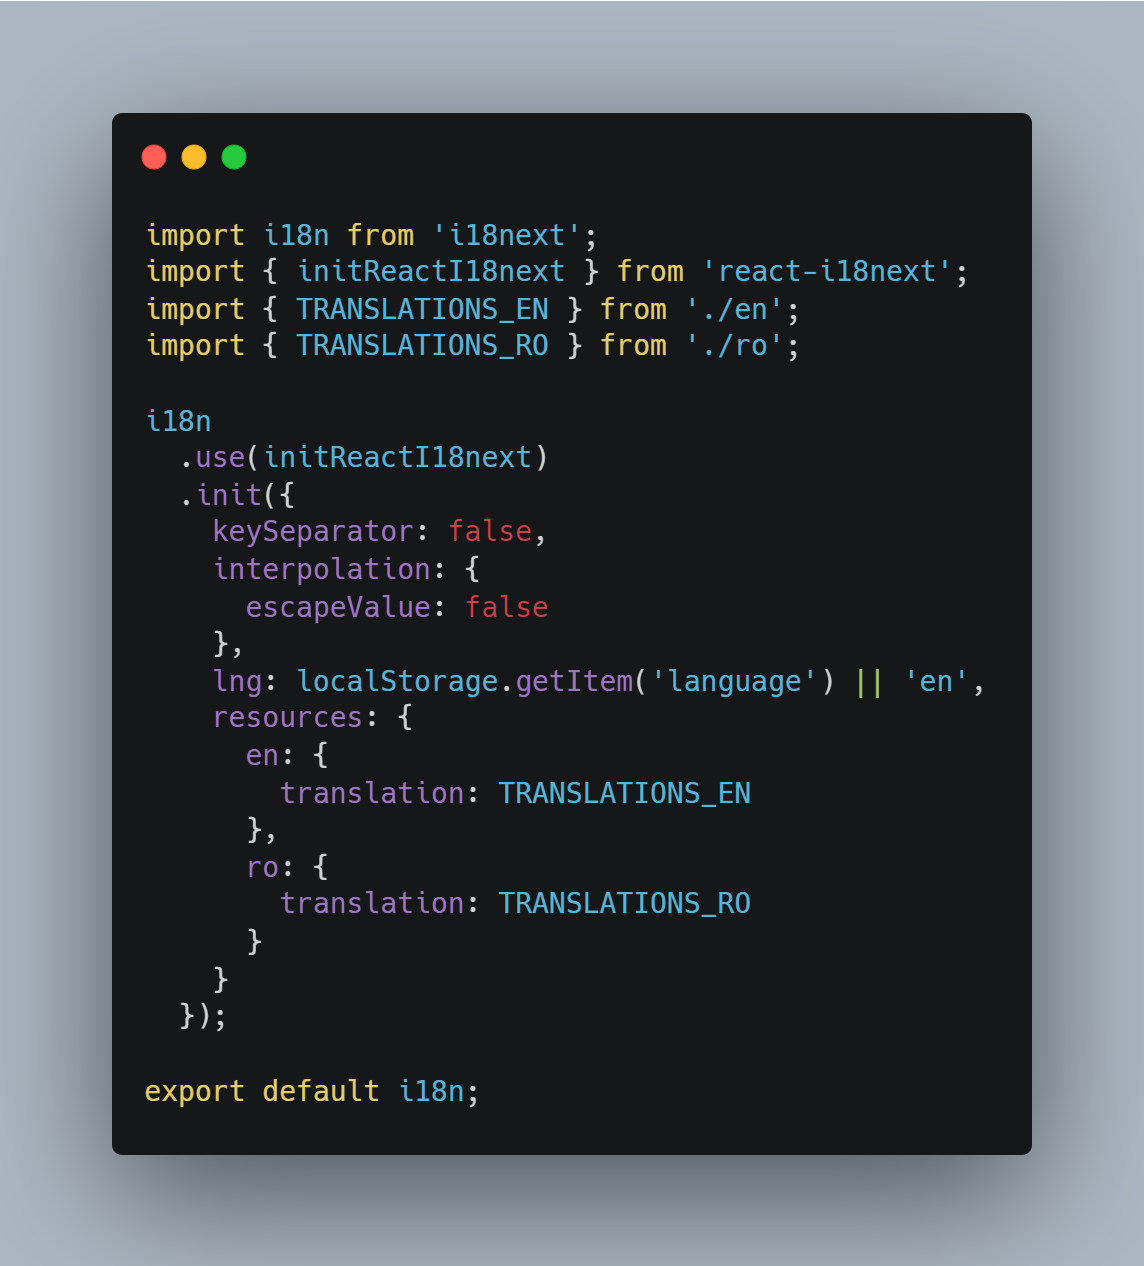
\includegraphics[width=150mm, height=150mm]{figs/i18nInstance.png}
	\caption{Configurare i18n}
	\label{fig:i18nInstance}
\end{figure}

\subsubsection{Services}
Pentru partea de servicii API și comunicare cu serverul, Axios este o librărie care ajută la creare request-urilor HTTP la endpoint-urile REST pentru a executa operații de stocare, citire, actualizare, ștergere (CRUD).\\
Folosind Axios cu un URL și, opțional un body, se obține un Promise care returnează un răspuns, după cum se poate vedea în figura \ref{fig:axiosPromise}.
\begin{figure}[h]
	\centering
	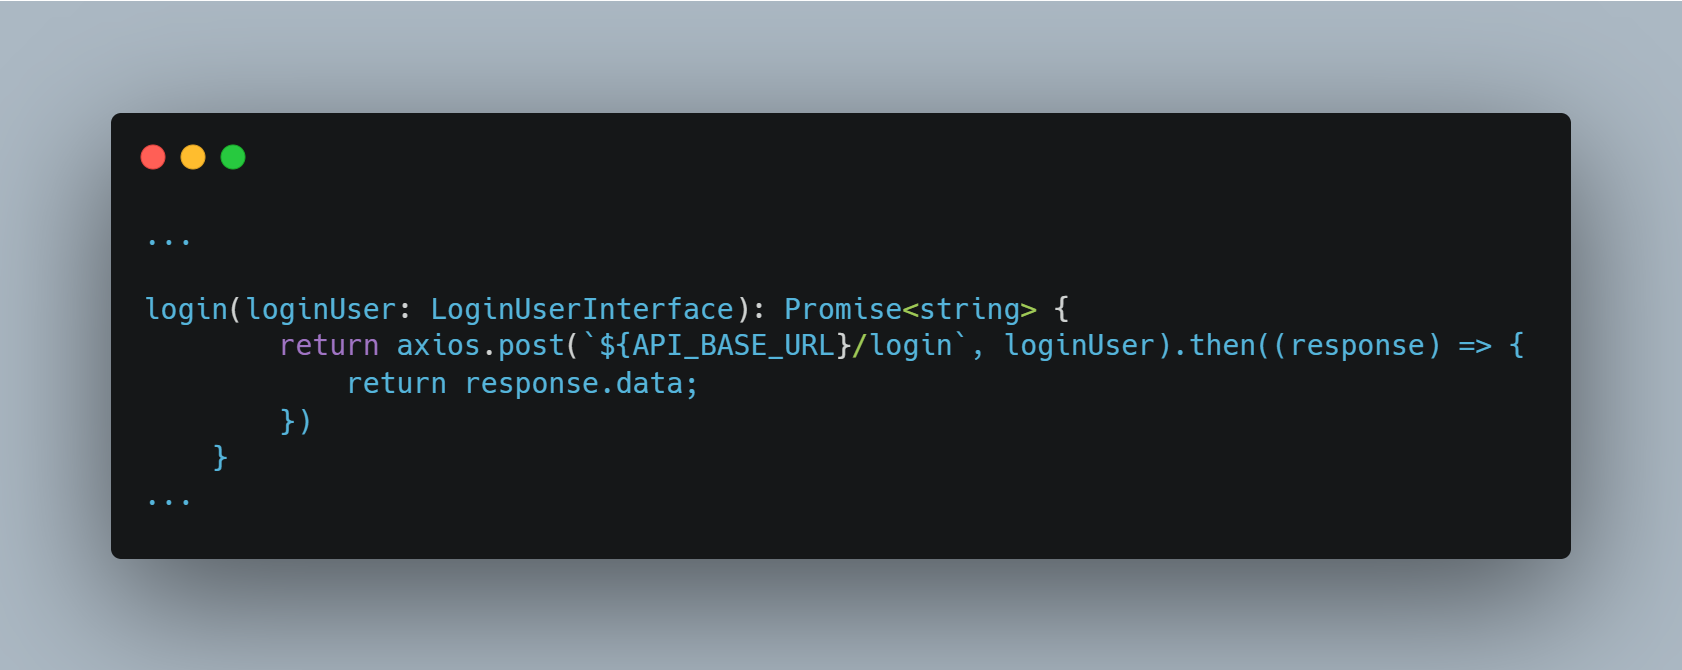
\includegraphics[width=150mm]{figs/axiosPromise.png}
	\caption{Structură request Axios}
	\label{fig:axiosPromise}
\end{figure}

\subsubsection{Components}
Componentele folosite în aplicație sunt din librările Ant Design, iar graficele sunt din librăria recharts. Pentru customizarea ambelor componente s-a folosit styled-components, cu o metodă de a aplica stilul numită CSS-in-JS. \\
Un exemplu de aplicare a stilului pe o componentă se poate vedea în figura \ref{fig:cssStyle}, iar rezultatul final în figura \ref{fig:notFoundPage}.
Se crează o componentă reutilizabilă numită Button404 (această componentă apare în pagina Not Fount) și moștenește stilul inițial al componentei din AntD prin {\it styled(Button)}. \\

\noindent Customizare componentei începe acum, când este setată o culoare de background pentru buton iar scrisul trebuie să fie alb (color: white). Se setează dimensiunilor butonului și un border-radius de 12 pixeli pentru a rotunji marginile butonului. 
\begin{figure}[h]
	\centering
	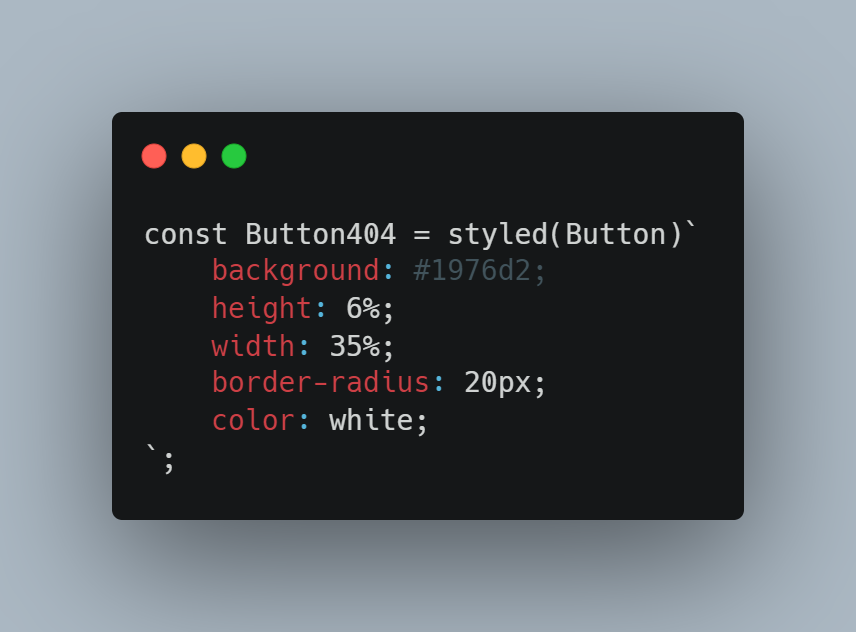
\includegraphics[width=100mm]{figs/cssStyle.png}
	\caption{Mod de aplicare a stilului folosind styled-components pe o componentă AntD}
	\label{fig:cssStyle}
\end{figure}

\newpage

\begin{figure}[h]
	\centering
	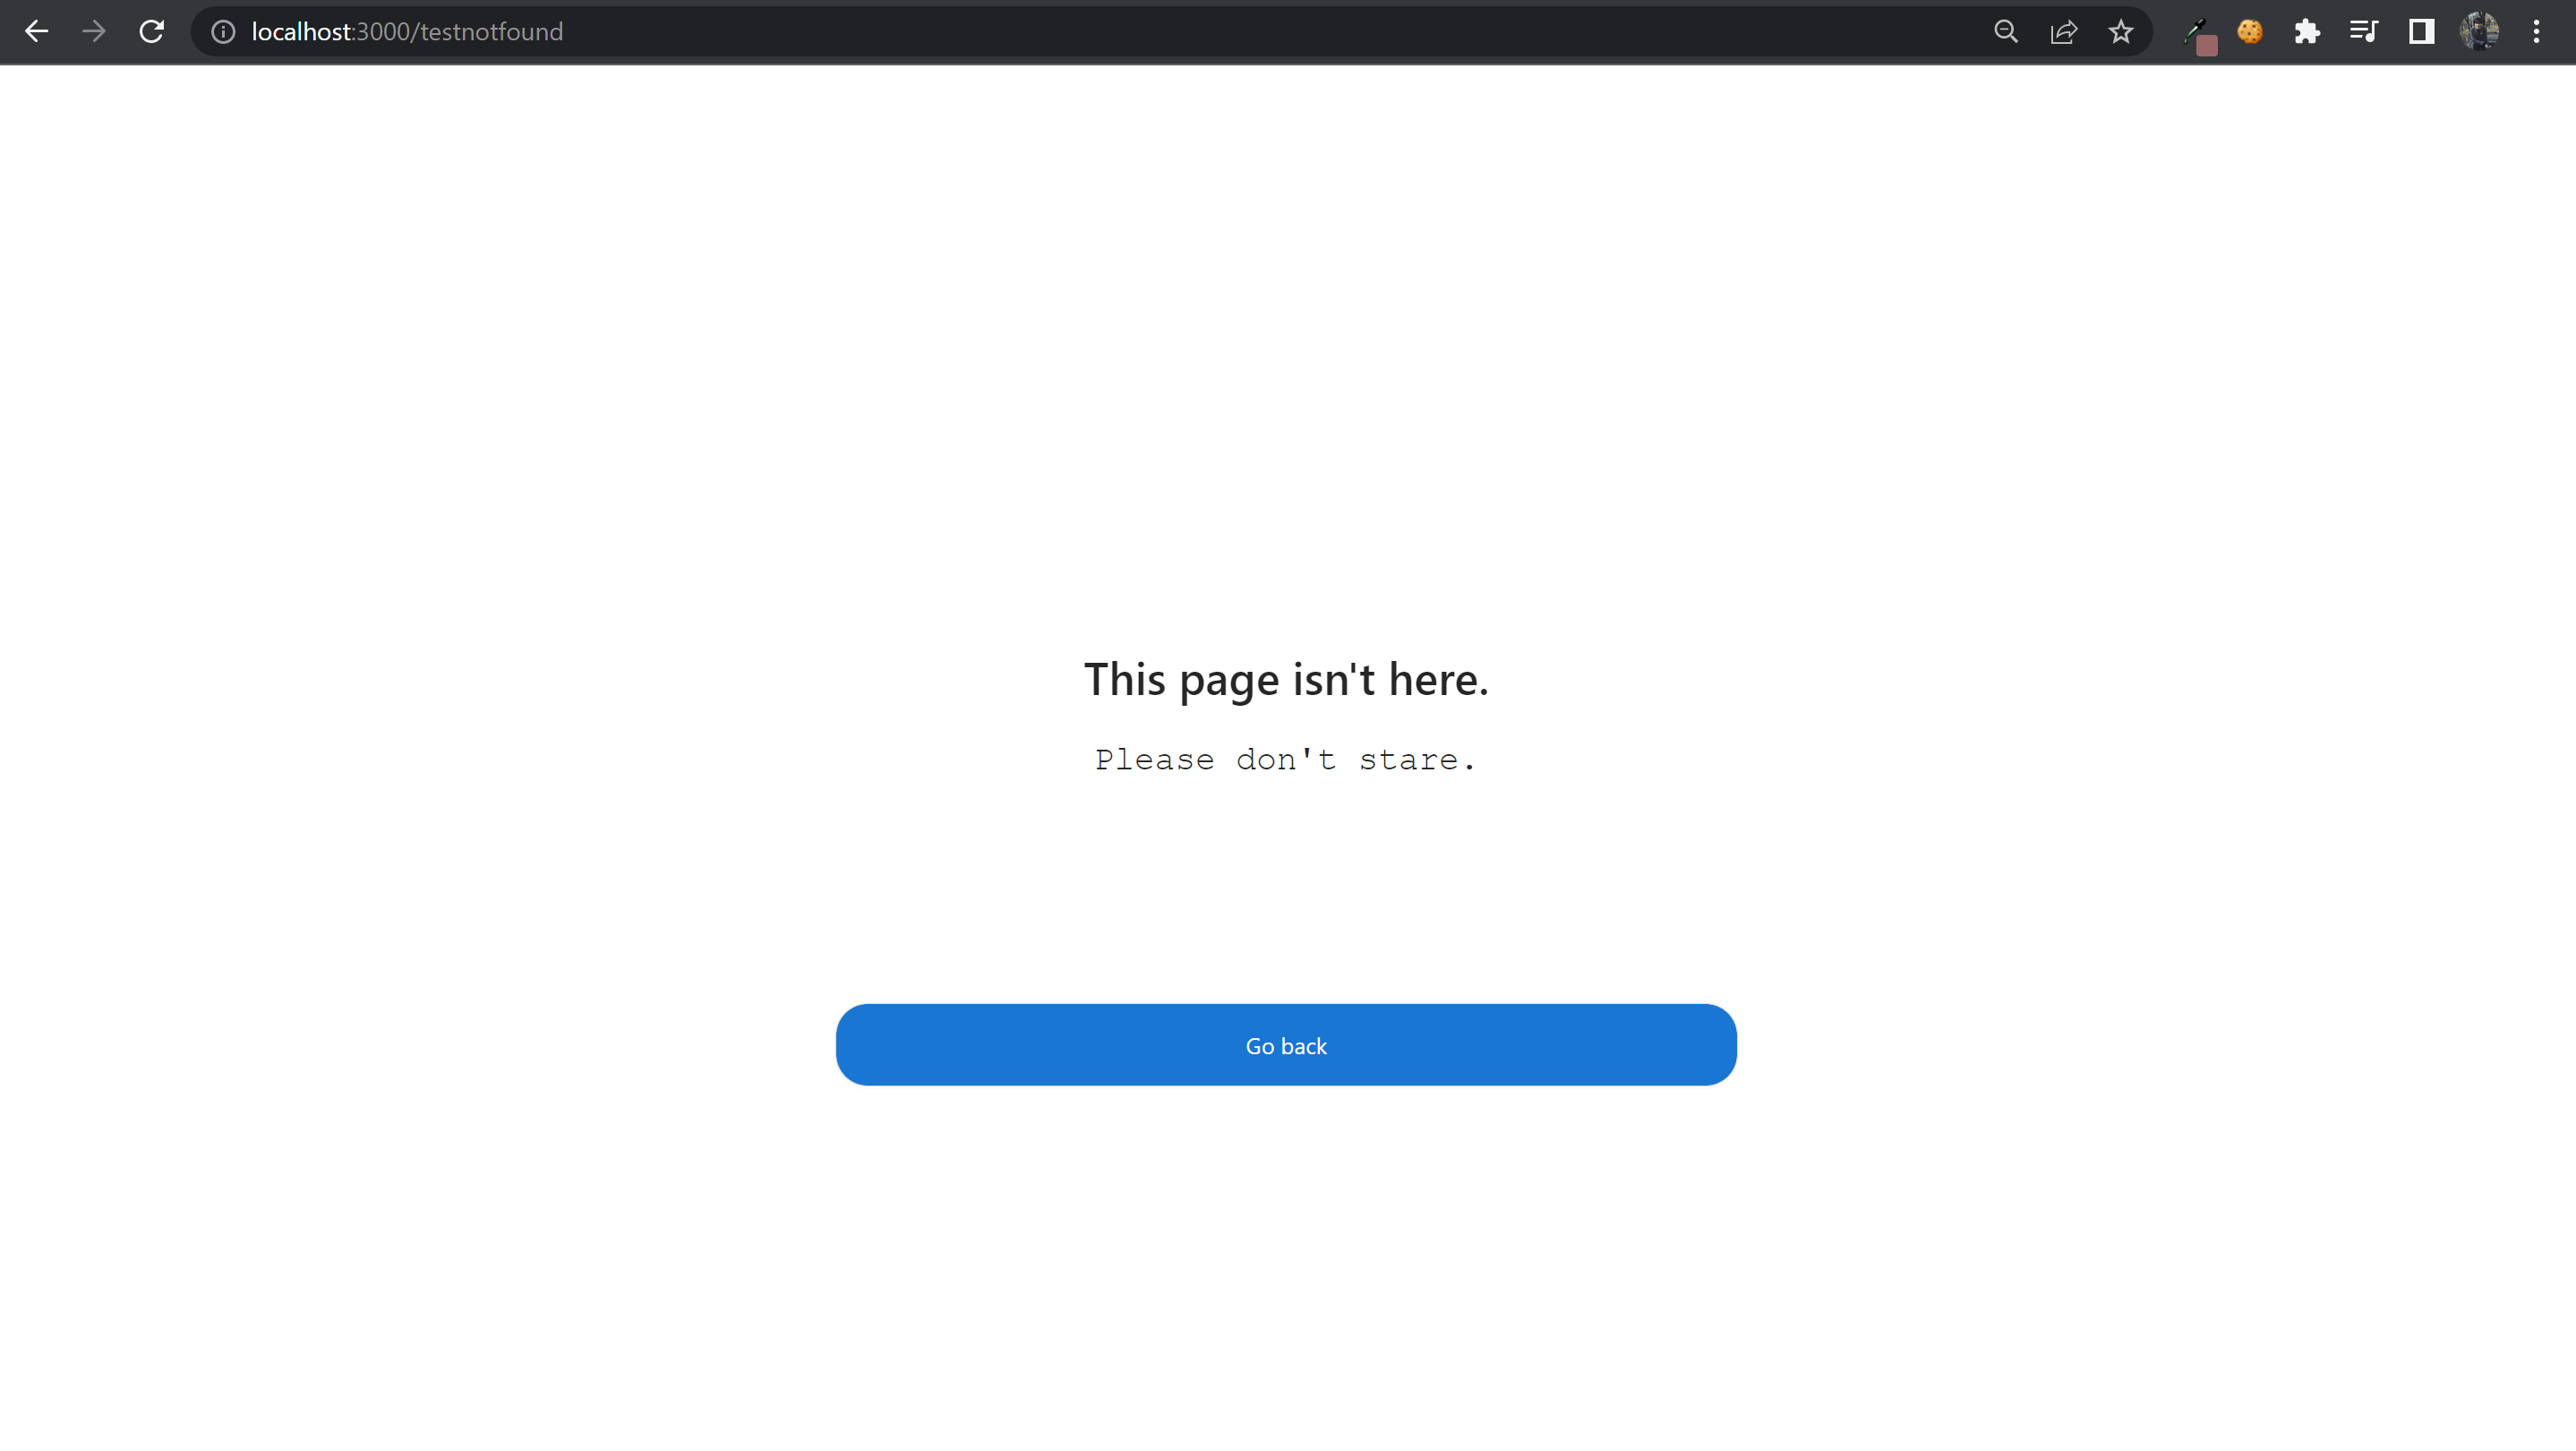
\includegraphics[width=100mm]{figs/notFoundPage.png}
	\caption{Stilul aplicat pe butonul din pagina de Not Found}
	\label{fig:notFoundPage}
\end{figure}

\begin{figure}[h]
	\centering
	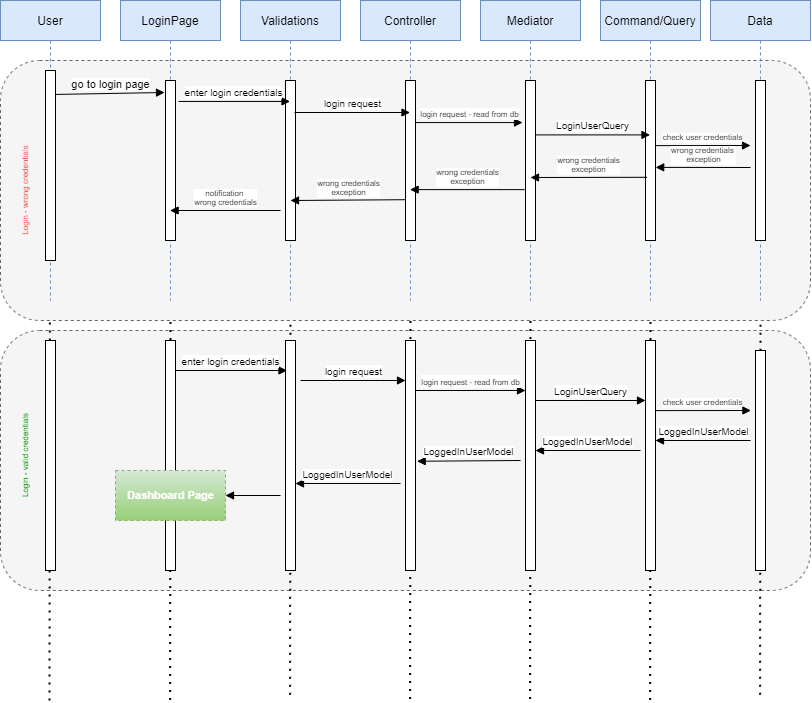
\includegraphics[width=150mm]{figs/sequnce.png}
	\caption{Diagramă de secvență pentru logarea în aplicație}
	\label{fig:sequnce}
\end{figure} 

\ \\ 
\section{Analizarea textului}
Aplicația realizează inferența pentru analiza sentimentelor din textele analizate, pentru sumarizarea textului și pentru extragerea cuvintelor cheie.\\
Hugging Face Inference API este accesat printr-un request HTTP, incluzând în body-ul requestului textul de la utilizator.\\

Cuvintele cheie sau expresiile sunt extrase din textul original și sunt evidențiate atât în partea de text original, cât și în partea de text sumarizat din pagina de Dashboard din frontend.\\
După extragerea cuvintelor cheie, acestea sunt salvate în baza de date, de unde se fac următoarele procesări, în funcție de inputul utilizatorului: \\

Pentru generarea graficului cu cele mai populare subiecte dintr-o anumită perioadă, se transmite o cerere cu perioada la server.\\
Mai departe, serverul caută în baza de date înregistrarile care corespund perioadei căutate și le contorizează în funcție de nume.
La final, rezultatul transmis este o listă de 10 elemente care conține obiecte constituite din numele cuvintelor și numărul de apariții, în acest fel fiind generat graficul de trending.\\

Pentru generarea graficului de evoluție al unui cuvânt cheie sau expresii, inputul trebuie să conțină perioada și cuvântul/cuvintele cautate.
Se face o căutare a înregistrărilor din baza de date care corespund perioadei căutate și al cărui nume corespunde cu inputul utilizatorului.\\
Înregistrarările care corespund căutării sunt ordonate apoi după data în care au fost salvate.
Rezultatul acestui filtru este o listă care conține obiecte constituite din ziua înregistrarii și numărul de apariții din acea zi.\\

WordCloud-ul este o colecție de cuvinte sau expresii de diferite mărimi. \\
Pentru generarea acestuia, la fel ca pentru graficul de trending, este nevoie de numărul de apariții pentru fiecare termen existent
în înregistrări. Diferența dintre cele două este că graficul de trending care este limitat la 10 elemente.\\
În funcție de numărul de înregistrări pentru un anumit termen, dimensiunea acestuia o sa varieze atunci când este afișat.
 % \chapter{Proiectare de Detaliu și Implementare}

\chapter{Testare și Validare}
\pagestyle{fancy}

\section{Testare backend}
Pentru partea de backend, s-a realizat testare automată a API-urilor, utilizând Swagger. 
Conform definiției de pe Wikipedia pentru API~\cite{API}, este o interfață de programare a aplicației, care permite mai multor dispozitive să comunice între ele. \\
Așadar, trebuie să ne asigurăm că informațiile transmise bidirecțional sunt corecte, atât din punct de vedere al URL-ului utilizat (acesta este modul în care se va face legătura între backend și frontend), cât și din punct de vedere al răspunsului și formatul acestuia.

\subsection{Testare login cu crendențiale greșite}
În cazul încercării de logare în aplicație când utilizatorul introduce credențialele greșite, răspunsul va fi sugestiv și nu va fi logat în aplicație, după cum se poate vedea în figurile \ref{fig:loginWrong1} și \ref{fig:loginWrong2}.
\begin{figure}[H]
	\centering
	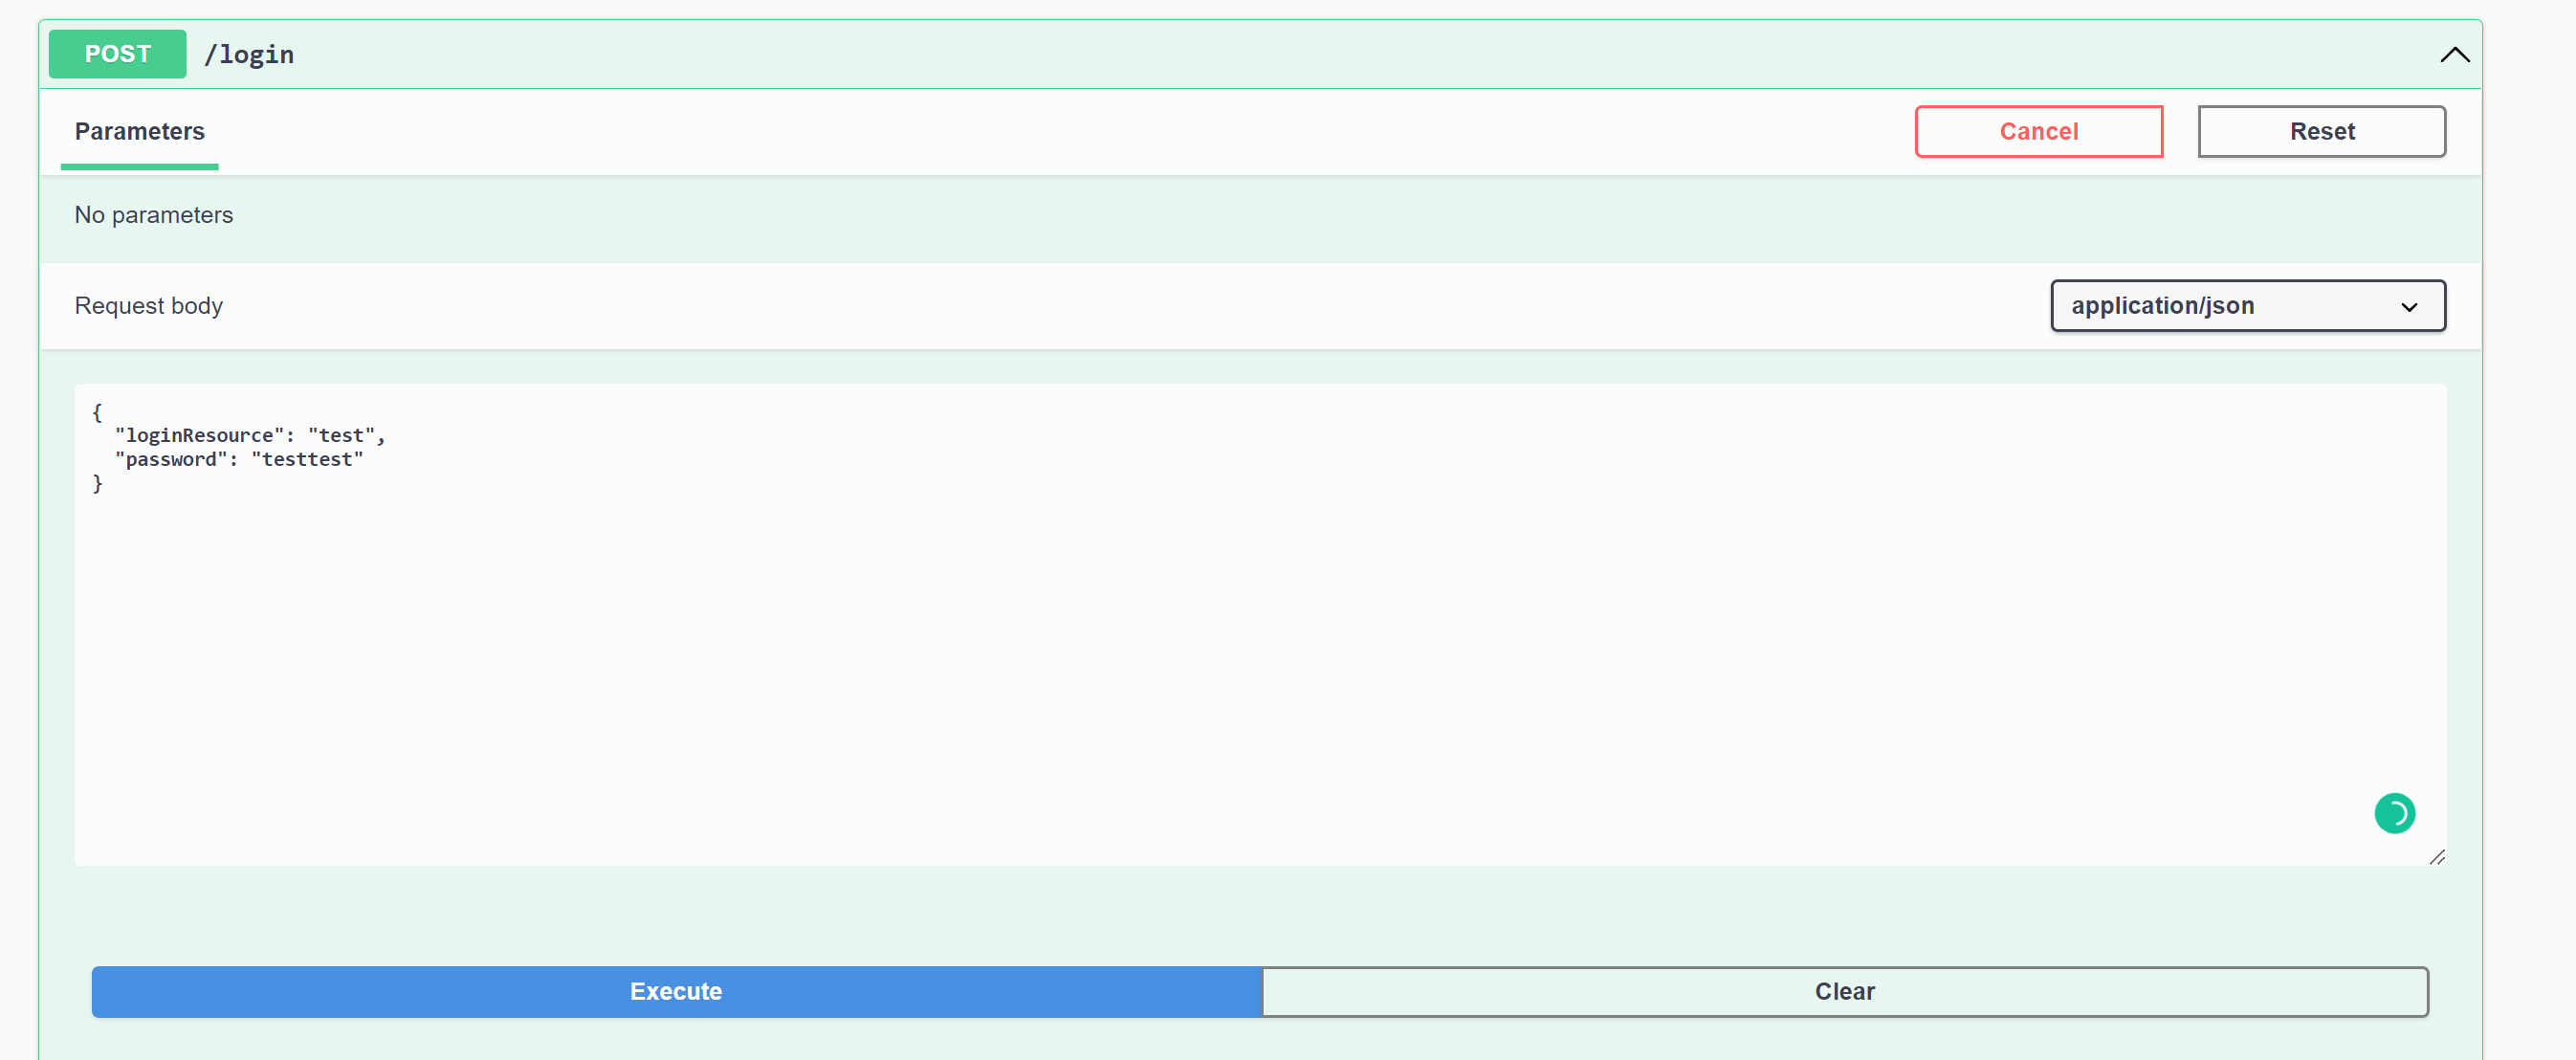
\includegraphics[width=100mm, scale=2]{figs/loginWrong1.png}
    \caption{Request - Login cu credențiale greșite}
	\label{fig:loginWrong1}
\end{figure}

\begin{figure}[H]
	\centering
	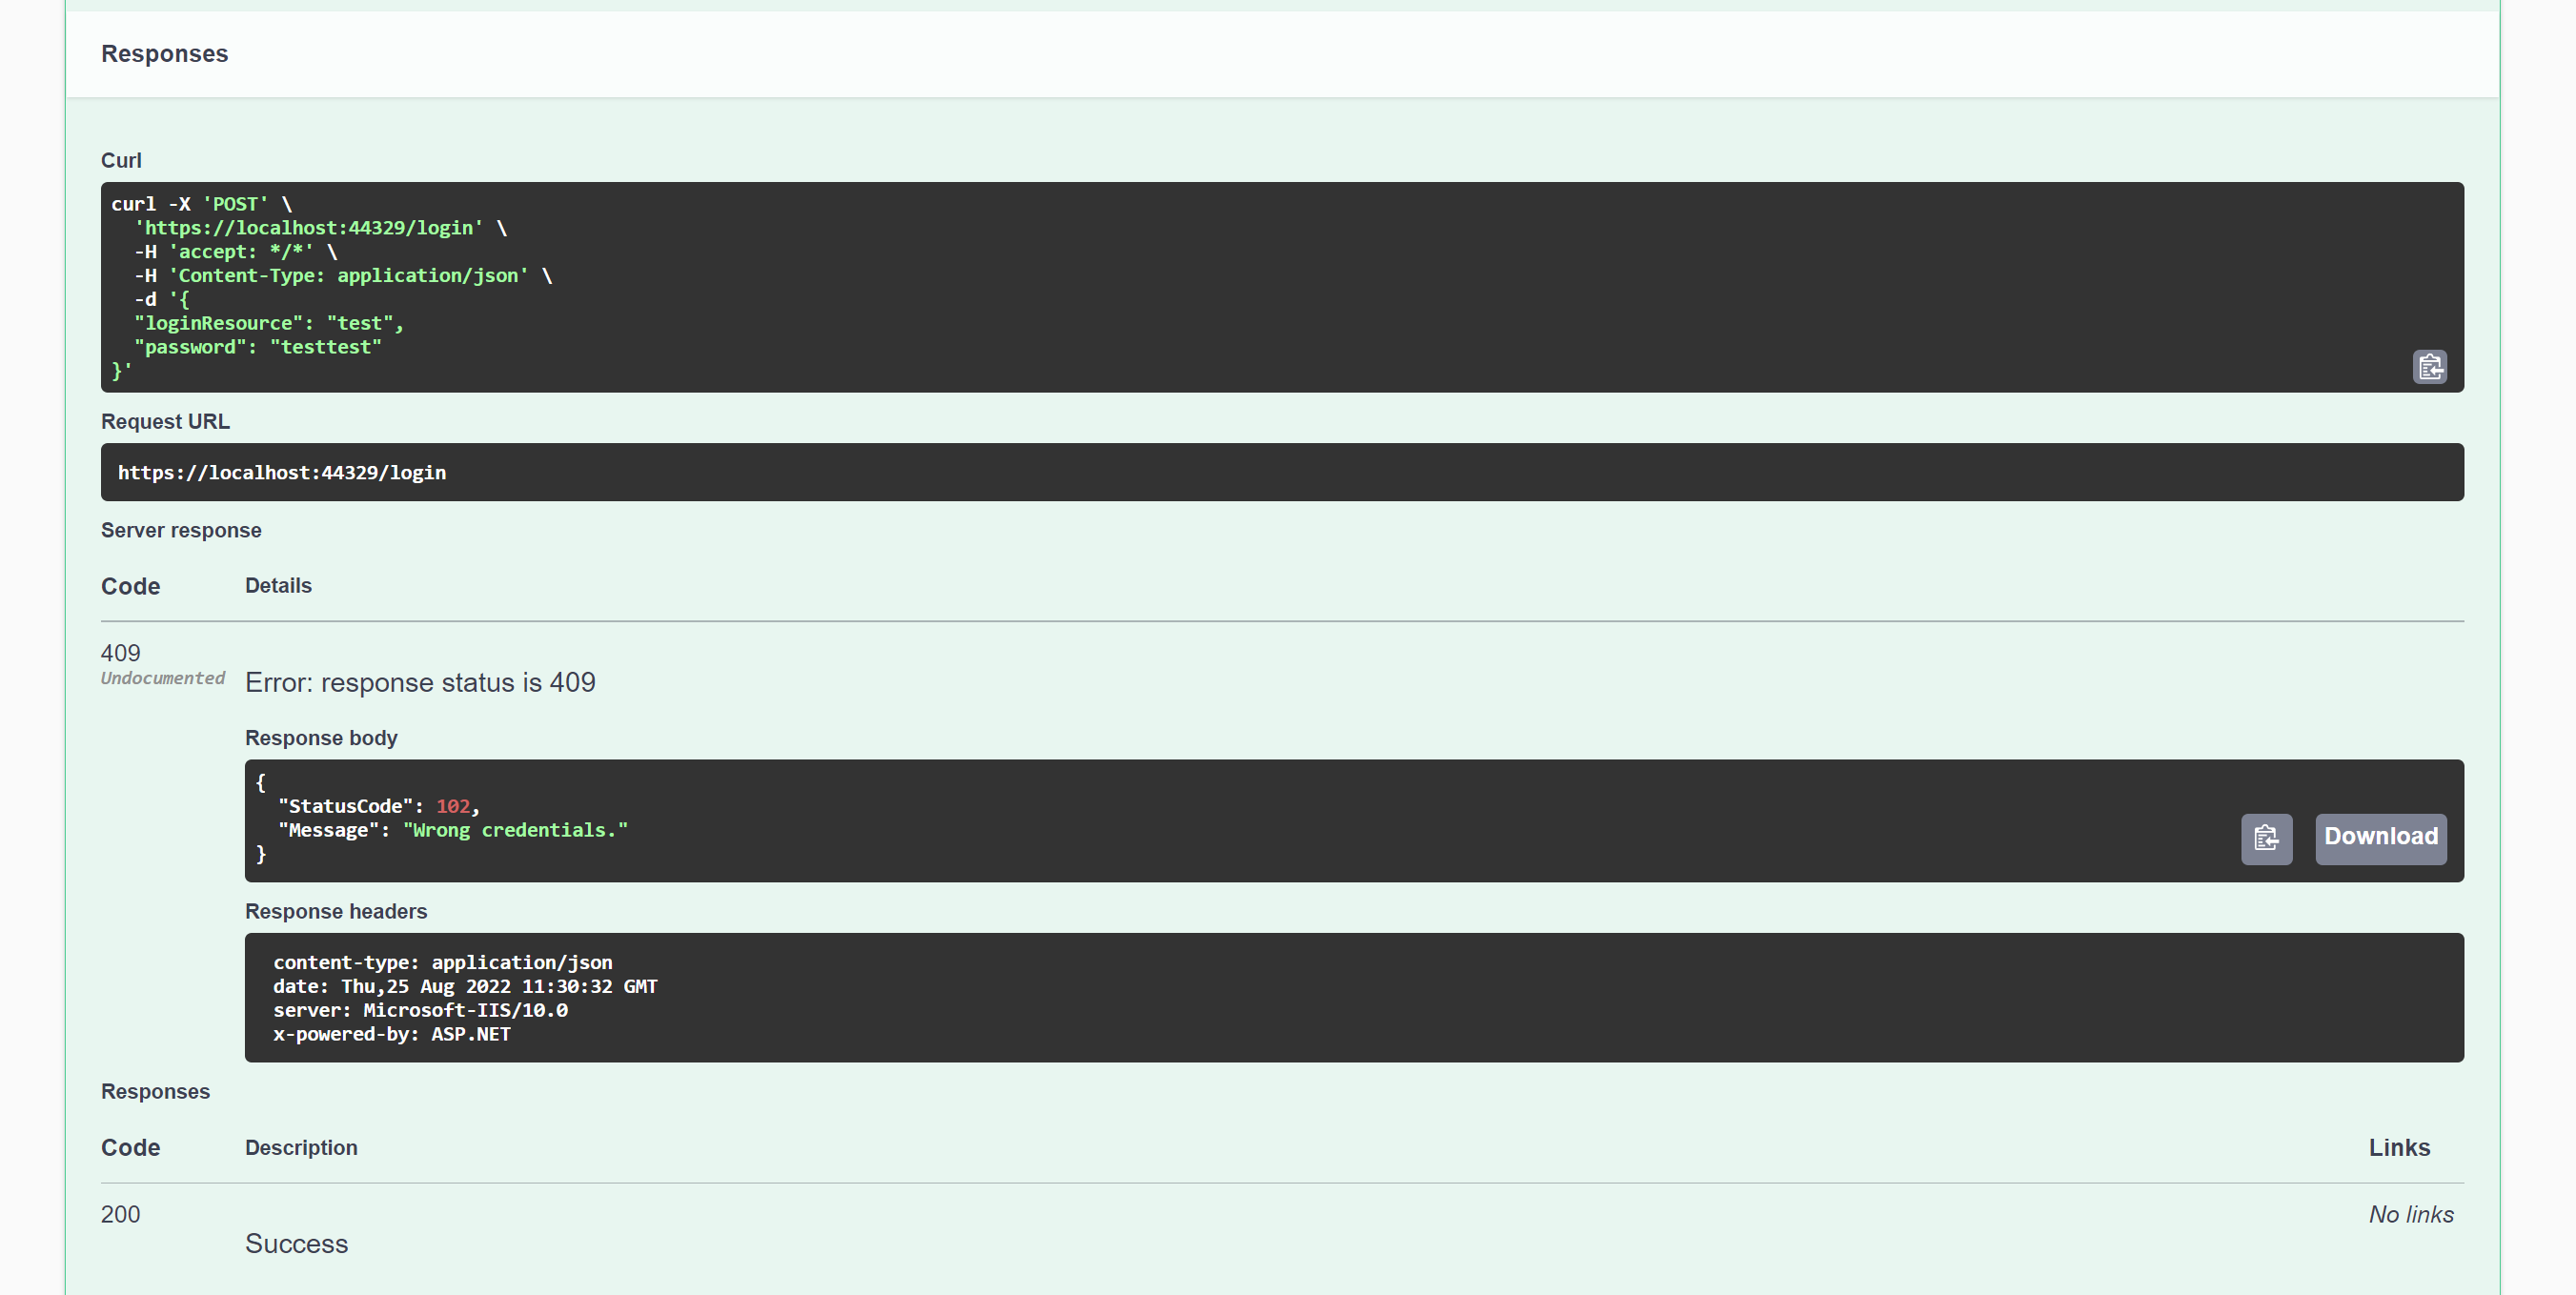
\includegraphics[width=100mm, scale=2]{figs/loginWrong2.png}
    \caption{Response - Login cu credențiale greșite}
	\label{fig:loginWrong2}
\end{figure}

\subsection{Testare login cu crendențiale corecte}
În cazul încercării de logare în aplicație când utilizatorul introduce credențialele corecte, răspunsul trimis la frontend va fi compus din Id-ul userului pentru a fi salvat în context și token-ul JWT generat, după cum se poate vedea în figurile \ref{fig:login1} și \ref{fig:login2}.

\begin{figure}[H]
	\centering
	\includegraphics[width=100mm, scale=2]{figs/login1.png}
    \caption{Request - Login cu credențiale corecte}
	\label{fig:login1}
\end{figure}

\begin{figure}[H]
	\centering
	\includegraphics[width=100mm, scale=2]{figs/login2.png}
    \caption{Response - Login cu credențiale corecte}
	\label{fig:login2}
\end{figure}
\subsection{Testare editare detalii utilizator când un câmp este gol}
În cazul încercării de editare a detaliilor utilizatorului când un câmp este gol, deși ar trebui să conțină informație sub formă de string, răspunsul va fi generat de constrângerea validatorului creat cu ajutorul Fluent Validation,
după cum se poate vedea în figurile \ref{fig:editWrong1} și \ref{fig:editWrong2}.
\begin{figure}[H]
	\centering
	\includegraphics[width=100mm, scale=2]{figs/editWrong1.png}
    \caption{Request - Editare detalii personale când un câmp este gol}
	\label{fig:editWrong1}
\end{figure}

\begin{figure}[H]
	\centering
	\includegraphics[width=100mm, scale=2]{figs/editWrong2.png}
    \caption{Response - Editare detalii personale când un câmp este gol}
	\label{fig:editWrong2}
\end{figure}


\section{Testare frontend}
Pentru partea de frontend, testarea s-a realizat manual, la nivelul fiecărei pagini, pentru a testa dacă funcționalitatea este cea așteptată în funcție de inputul utilizatorului.
Rezultatele se pot observa în figurile \ref{fig:testareFE1}, \ref{fig:testareFE2} și \ref{fig:testareFE3}.

\begin{figure}[h]
	\centering
	\includegraphics[height=100mm]{figs/testareFE1.png}
    \caption{Testare modul frontend - partea 1}
	\label{fig:testareFE1}
\end{figure}

\begin{figure}[ht]
	\centering
	\includegraphics[height=100mm]{figs/testareFE2.png}
    \caption{Testare modul frontend - partea 2}
	\label{fig:testareFE2}
\end{figure}

\begin{figure}[ht]
	\centering
	\includegraphics[height=100mm]{figs/testareFE3.png}
    \caption{Testare modul frontend - partea 3}
	\label{fig:testareFE3}
\end{figure}
\ \\
\section{Testare analiză a textului}
Pe partea de analiză de text, testarea s-a realizat prin compararea empirică a mai multor modele din Hugging Face utilizând diferite texte. % \chapter{Testare și Validare}

\chapter{Manual de Instalare și Utilizare}
\pagestyle{fancy}

\section{Instalare}
\subsection{Condiții prealabile generale}
\noindent Resursele hardware necesare pentru instalarea și rularea aplicației sunt:
\begin{itemize}
    \setlength\itemsep{0.5em}
    \item Sistem de operare: Windows
    \item Arhitectura sistemului de operare: x64
    \item Memorie RAM: minim 8GB
\end{itemize}

\subsection{Condiții prealabile pentru baza de date}
Este de preferat să fie instalate versiunile cele mai noi, {\it Long Term Support}.\\

\noindent Pentru instalarea resurselor necesare bazei de date, este nevoie de:
\begin{itemize}
    \setlength\itemsep{0.5em}
    \item \href{https://www.microsoft.com/en-us/sql-server/sql-server-downloads}{\color{blue}SQL Server}
    \begin{itemize}
        \setlength\itemsep{0.5em}
        \item Se descarcă din secțiunea Free Specialized Edition -> Developer
        \item Se deschide fișierul descărcat și se urmează instrucțiunile până la tipul instalării. Aici se va selecta {\it Basic}
        \item După ce instalarea a fost finalizată cu succes, se apasă butonul de {\it Install SSMS} 
        \item După ce SSMS a fost instalat, deschideți Microsoft SQL Server Management Studio
        \item Pentru Server Type se poate păstra Database Engine, iar pentru Authentication se va selecta Windows Authentication
    \end{itemize}

    \item \href{https://docs.microsoft.com/en-us/sql/ssms/download-sql-server-management-studio-ssms?view=sql-server-ver16}{\color{blue}SQL Server Management Studio (SSMS)}
    \begin{itemize}
        \setlength\itemsep{0.5em}
        \item Se deschide fișierul descărcat, se va selecta locația unde se dorește a fi instalat, apoi se apasă pe butonul de Install
        \item După ce instalarea e completa, e nevoie să fie restartat calculatorul 
    \end{itemize}
\end{itemize}

După ce toate instalările au fost finalizate cu succes, se pot crea baze de date, tabele și se pot efectua diferite comenzi și interogări.
\subsection{Condiții prealabile pentru modulul de backend}
Aplicația a fost creată utilizând .NET 6. De preferat, a se folosi această versiune, pentru că este posibil să fie modificări în versiunile ulterioare sau anterioare ce implică o sintaxă diferită.
Spre exemplu, la trecerea de la .NET 5 la .NET 6, fișierele Program.cs și Startup.cs au fost comasate.
\begin{itemize}
    \setlength\itemsep{0.5em}
    \item \href{https://dotnet.microsoft.com/en-us/download}{\color{blue}.NET 6}
    \begin{itemize}
        \setlength\itemsep{0.5em}
        \item Se apasă butonul Download {\it .NET SDK x64}, versiunea .NET 6.0, LTS
        \item Din pagina unde s-a făcut redirecționarea după apăsarea pe buton, se va selecta Installer-ul potrivit pentru sistemul de operare
        \item După descărcare, se va deschide fișierul executabil și se vor urma instrucțiunile
        \item Se poate testa într-un command line dacă instalarea s-a făcut cu succes, scriind {\it dotnet --info}
    \end{itemize}
    \item IDE: \href{https://www.jetbrains.com/rider/download/#section=windows}{\color{blue}Rider}
    \begin{itemize}
        \setlength\itemsep{0.5em}
        \item Se poate descărca de pe site-ul oficial sau din \href{https://www.jetbrains.com/toolbox-app/}{\color{blue}Jetbrains Toolbox}
        \item Se acceptă toate setările default
    \end{itemize}
\end{itemize}

\subsection{Condiții prealabile pentru modulul de frontend}
\begin{itemize}
    \setlength\itemsep{0.5em}
    \item Node v16.13.0
    \begin{itemize}
        \setlength\itemsep{0.5em}
        \item Se poate descărca \href{https://nodejs.org/en/download/}{\color{blue}de aici}
        \item Se acceptă toate setările default
    \end{itemize}
    \item Node Package Manager (npm) 8.1.0
    \begin{itemize}
        \setlength\itemsep{0.5em}
        \item Se poate descărca \href{https://nodejs.org/en/download/}{\color{blue}de aici}
        \item Se acceptă toate setările default
    \end{itemize}
    \item Text Editor: Visual Studio Code
    \begin{itemize}
        \setlength\itemsep{0.5em}
        \item Se poate descărca \href{https://code.visualstudio.com/download}{\color{blue}de aici}
        \item Se acceptă toate setările default
    \end{itemize}
\end{itemize}

\section{Rulare}
\subsection{Setup baza de date}
Dacă apar erori legate de baza de date, trebuie să se creeze una manual care să coincidă cu numele din fișierul appsettings.json din modulul de backend.
\subsection{Rulare modul backend}
La prima utilizare, trebuie să se importe proiectul și să se ruleze configurarea IIS Express. Se va rula comanda {\it dotnet ef database update} pentru a fi actualizată baza de date și pentru a fi create tabelele care vor fi ulterior folosite.
\begin{figure}[ht]
	\centering
	\includegraphics[width=150mm]{figs/configBackend.png}
    \caption{Configurări rulare backend}
	\label{fig:configBackend}
\end{figure}

Aplicația va deschide în broswer Swagger cu {\it https://localhost:44329/swagger/index.html}, un instrument care permite testarea și documentarea serviciilor REST.
\begin{figure}[H]
	\centering
	\includegraphics[width=150mm]{figs/swagger.png}
    \caption{Swagger, instrument pentru testarea endpointurilor aplicatiei}
	\label{fig:swagger}
\end{figure}
În acest moment, backend-ul rulează pe portul 44329 la care se va conecta modulul de frontend pentru a folosi API-ul creat.
\subsection{Rulare modul frontend}
După instalarea editorului de text Visual Studio Code, se va importa proiectul aici. Pentru a fi instalate toate dependințele necesare rulării proiectului, 
se va rula în terminal {\it npm init}. 
După ce toate dependințele au fost descărcate și instalate cu succes, se poate rula în terminal comanda {\it npm start}. După ce aplicația a pornit, se va deschide în broswer un tab de React App cu {\it http://localhost:3000/login}.
\begin{figure}[ht]
	\centering
	\includegraphics[width=150mm]{figs/startAppFrontend.png}
    \caption{Rulare frontend}
	\label{fig:startAppFrontend}
\end{figure}

\section{Manual de utilizare}
La pornirea aplicației, dacă nu a folost logat niciun alt utilizator înainte, prima pagină care se va deschide va fi pagina de login.
În funcție de preferințele utilizatorului, acesta poate modifica limba aplicației cu ajutorul switch-ului de limbi. Această setare poate fi modificată și mai târziu.

Pentru crearea unui cont nou, se va apăsa pe butonul indicat în figura \ref{fig:loginPage}. După ce am ajuns pe pagina de Register sau Creare cont nou, utilizatorul va trebui să completeze datele.
Aplicația ofera feedback vizual utilizatorului atunci când informațiile introduse de acesta în pagină nu respectă una dintre condițiile de număr minim, număr maxim de caractere format corect pentru email. Acest lucru se poate vedea în figura \ref{fig:createAccount}.
După ce toate câmpurile au fost corect completate din punct de vedere al restricțiilor menționate mai sus, se mai fac 2 verificări - numele de utilizator și email-ul să fie unice.
În cazul în care una din ele nu respectă condiția de unicitate, utilizatorul va fi notificat cu un mesaj corespunzător pentru a putea lua măsuri, după cum se poate vedea în figura.

\begin{figure}[ht]
	\centering
	\includegraphics[width=100mm]{figs/loginPage.png}
    \caption{Pagina de login}
	\label{fig:loginPage}
\end{figure}

\begin{figure}[ht]
	\centering
	\includegraphics[width=150mm]{figs/createAccount.png}
    \caption{Pagina de creare cont nou}
	\label{fig:createAccount}
\end{figure}

După ce contul a fost creat cu succes, se ajunge la pagina de login, unde trebuie completate credențialele pentru a putea intra în aplicație. 
În cazul în care credențialele nu sunt corecte, utilizatorul va fi notificat, după cum se poate vedea în figura \ref{fig:wrongCredentialsLogin}. 
\begin{figure}[H]
	\centering
	\includegraphics[width=150mm]{figs/wrongCredentialsLogin.png}
    \caption{Credențiale greșite la logarea în aplicație}
	\label{fig:wrongCredentialsLogin}
\end{figure}
În acest moment, utilizatorul nu este logat și are acces doar la pagina de Login și pagina de Register, toate celelalte pagini din aplicație sunt inaccesibile, iar daca va încerca să ajungă la una din ele din URL, 
acesta va fi redirecționat automat la pagina de login. 

Când credențialele corecte au fost completate, utilizatorul va intra în aplicație. În acest moment, are acces la toate paginile și resursele din aplicație, dar nu are acces la paginile de Login și Register. 

După logare, pe pagina de Dashboard, utilizatorul poate adauga în caseta de text un text pe care dorește să îl analizeze. Nu poate trece mai departe, la componentele de afișare a informațiilor detaliate
până când nu există input în casetă; altfel, va primi un mesaj specific, cum e în figura \ref{fig:dashboardInput}.
\begin{figure}[H]
	\centering
	\includegraphics[width=150mm]{figs/dashboardInput.png}
    \caption{Încercare de a efectua o analiză fără input de la utilizator}
	\label{fig:dashboardInput}
\end{figure}

După ce userul a adăugat textul pe care dorește să îl analizeze și apasă pe butonul SUBMIT, rezultatele vor apărea și un buton de mers la următoarea pagină se va încărca, cum apare în figura \ref{fig:seeMoreButton}.
\begin{figure}[H]
	\centering
	\includegraphics[width=150mm]{figs/seeMoreButton.png}
    \caption{Buton pentru a merge în pagina de vizualizare a analizei detaliate a textului}
	\label{fig:seeMoreButton}
\end{figure}

După ce ajungem în pagina cu informații detaliate despre textul analizat, putem observa pe primul rând 2 carduri în care este afișat textul original și textul sumarizat. \\
În următorul card, avem statisticile sentimentelor - pozitiv, neutru și negativ. Aceste informații se pot vedea în figura \ref{fig:seeMore1}.
\begin{figure}[H]
	\centering
	\includegraphics[width=150mm]{figs/seeMore1.png}
    \caption{Rezultate analiza - partea 1}
	\label{fig:seeMore1}
\end{figure}

În ultimul card, care este unul interactiv, utilizatorul poate alege dintre cuvintele cheie extrase din text și perioada dorită pentru a genera graficul aparițiilor, după cum se poate vedea în figura \ref{fig:seeMore2}. \\
În acest grafic, în primul dropdown sunt cuvintele cheie extrase din text. Acestea pot fi observate fiind evidențiate prin subliniere în textul original din figura \ref{fig:seeMore1}. 
Rezultatul pe grafic poate fi observat în figura \ref{fig:keywordsEvolution}.

\begin{figure}[H]
	\centering
	\includegraphics[width=150mm]{figs/seeMore2.png}
    \caption{Rezultate analiza - partea 2}
	\label{fig:seeMore2}
\end{figure}
\begin{figure}[H]
	\centering
	\includegraphics[width=150mm]{figs/keywordsEvolution.png}
    \caption{Rezultate analiza - evoluție cuvinte cheie}
	\label{fig:keywordsEvolution}
\end{figure}

În acest punct, se poate observa butonul de salvare a articolului analizat, împreună cu rezultatele obținute în istoricul personal al utilizatorului, în figura \ref{fig:saveArticle}.  \\
Informațiile pot fi redeschise ulterior, în orice moment, din pagina de Dashboard, cum apar în figura \ref{fig:personalHistory}, apăsând butonul See More. De asemenea, articolele pot fi șterse din istoricul personal
al utilizatorului apăsând butonul Delete.
\begin{figure}[H]
	\centering
	\includegraphics[width=150mm]{figs/saveArticle.png}
    \caption{Buton de salvare articol}
	\label{fig:saveArticle}
\end{figure}
\begin{figure}[H]
	\centering
	\includegraphics[width=150mm]{figs/personalHistory.png}
    \caption{Istoricul analizelor de text salvate de utilizator}
	\label{fig:personalHistory}
\end{figure}

Pentru a edita informațiile contului utilizatorul, se accesează pagina de Profile. Câmpurile care pot fi modificate sunt Nume, Prenume, Nume de utilizator, Email, Parola. 
Singurele restricții în modificarea acestor câmpuri sunt ca Numele de utilizator și Email-ul să fie unice, neatribuite altui cont existent, altfel utilizatorul va fi notificat cu una dintre următoarele erori, ca în figura \ref{fig:editProfileUsername}.

\begin{figure}[H]
	\centering
	\includegraphics[width=150mm]{figs/editProfileUsername.png}
    \caption{Utilizatorul încearcă să își schimbe username-ul, dar acesta este deja atribuit altui cont}
	\label{fig:editProfileUsername}
\end{figure}

După ce utilizator a ales un nou username și/sau email care respectă condiția de unicitate, acesta va fi notificat că actualizarea detaliilor contului s-a făcut cu succes, cum apare în figura \ref{fig:editProfile}.
\begin{figure}[H]
	\centering
	\includegraphics[width=150mm]{figs/editProfile.png}
    \caption{Actualizare detalii cont cu succes}
	\label{fig:editProfile}
\end{figure}

În pagina de Manage, utilizatorul poate vedea topicele cele mai populare, adică cele mai des apărute cuvinte cheie sau expresii în analizele efectuate și de restul utilizatorilor.\\
În cazul în care utilizatorul a selectat o perioadă în care nu sunt înregistrate date, va fi notificat de acest lucru, ca în figura \ref{fig:trendingNoData}, altfel rezultatele vor fi afișate pe grafic, ca în figura \ref{fig:trending}. 
\begin{figure}[h]
	\centering
	\includegraphics[width=150mm]{figs/trendingNoData.png}
    \caption{Grafic pentru top 10 cele mai populare subiecte - niciun rezultat}
	\label{fig:trendingNoData}
\end{figure}

\begin{figure}[h]
	\centering
	\includegraphics[width=150mm]{figs/trending.png}
    \caption{Grafic pentru top 10 cele mai populare subiecte}
	\label{fig:trending}
\end{figure}

\newpage
Alt element important pe care utilizatorul îl poate vedea aici este un WordCloud, care este, de fapt, o colecție de cuvinte sau expresii de diferite mărimi, ca în figura \ref{fig:wordcloud}. Mărimea este determinată de numărul total de apariții.
\begin{figure}[ht]
	\centering
	\includegraphics[width=150mm]{figs/wordcloud.png}
    \caption{WordCloud}
	\label{fig:wordcloud}
\end{figure}

\ \\
Evoluția unui cuvânt cheie sau expresie poate fi observată într-o perioadă de timp selectată.\\
La fel ca în cazul topicelor populare, dacă nu există date salvate pentru perioada sau inputul selectat, utilizatorul va fi notificat de acest lucru, ca în figura \ref{fig:evolutionNoData}. 
\begin{figure}[h]
	\centering
	\includegraphics[width=150mm]{figs/evolutionNoData.png}
    \caption{Evoluția unui cuvânt cheie într-o anumită perioadă - niciun rezultat}
	\label{fig:evolutionNoData}
\end{figure}

\newpage
Altfel, în grafic se poate observa evoluția pe zile, ca în figura \ref{fig:evolution}.
\begin{figure}[t]
	\centering
	\includegraphics[width=150mm]{figs/evolution.png}
    \caption{Evoluția unui cuvânt cheie într-o anumită perioadă}
	\label{fig:evolution}
\end{figure} % \chapter{Manual de Instalare și Utilizare}

\chapter{Concluzii}
\pagestyle{fancy}

\section{Analiza rezultatelor obținute}
Aplicația realizată îndeplinește obiectivele setate la început, fiind un instrument de analiză detaliată a unui text cu specific financiar.\\
Reușind integrarea modelelor de procesare de limbaj natural în aplicația web, aceasta oferă, pe lângă funcționalități generale ale unei aplicații web, analiza sentimentelor financiare dintr-un text, 
sumarizarea textului și extragerea cuvintelor cheie.\\

Unul dintre obiectivele setate la început pentru aplicație era ca utilizatorul să poată lua o decizie financiară informată. 
Cu ajutorul analizei sentimentelor financiare, sunt obținute scoruri pentru fiecare dintre sentimentele negativ, neutru, pozitiv și acestea pot influența decizia utilizatorului.\\
De multe ori, un scor pozitiv ridicat poate fi perceput ca un lucru bun, la fel cum un scor negativ ridicat poate fi perceput ca un lucru rău.
Pentru cazurile excepționale când un scor negativ ridicat poate însemna și un lucru benefic pentru investitor, acesta trebuie determinat din context.\\

Textele analizate pot avea diferite dimensiuni și posibil, doar anumite părți sunt interesante pentru investitor. Deci dimensiunea unui text e măsurată în timp și se dorește un răspuns într-un timp scurt.\\
Autorul scrie în~\cite{LengthOfAnArticle} următoarea afirmație: {\it "If you are looking for a good rule of thumb, write content between 1,500 and 3,000 words."}. Continuând apoi cu o analiză a timpului
petrecut citind un anumit număr de cuvinte~\cite{TimePerWords}, considerând o viteză medie, pentru aproximativ 2000 de cuvinte o persoană va petrece aproximativ 6.7 minune per articol.\\

A citi nu e nici pe de parte un lucru rău, doar că aici se doresc informații în timp cât mai scurt pentru că se urmărește momentul potrivit. Așadar, intervine sumarizarea textului, alt obiectiv al acestei aplicații.
Utilizatorul va reduce timpul petrecut pentru citirea unui articol, extragând ideile principale, astfel încât să își poată da seama din context de motivul scorului sentimentelor rezultat.\\

Tot în acest scop, aplicația realizează și extragerea cuvintelor cheie, pentru a oferi o privire de perspectivă asupra a ce se întâmplă în acest moment.\\
Cu rezultatele obținute, utilizatorul poate vedea evoluția interesului general pentru un anumit subiect, cele mai populare 10 subiecte și anumite definiții pentru cuvintele cheie cheie extrase.\\

Pe lângă aceste funcționalități, aplicația web se concentrează și pe partea de securitate; întrucât utilizatorul poate să își salveze documente în istoricul personal, accesul altor persoane cu intenții rele trebuie să fie restricționat.
Acest lucru e realizat cu ajutorul tokenilor, rutelor protejate și parolele unice.

\newpage

\section{Dezvoltări și îmbunătățiri ulterioare}
Pentru partea de îmbunătățiri ulterioare, în primul rând, o funcționalitate necesară consider că ar fi o analiză a sentimentelor pe text, pe anumite părți din text selectate de utilizator.\\
Spre exemplu să existe 2 cursoare, unul pentru a fi poziționat la începutul textului care se dorește a fi analizat și alt cursor pentru a fi poziționat la finalul textului. 
Momentan, în aplicație, sentimentul financiar este obținut pentru tot textul analizat, așa că o îmbunătățire ar fi selectarea unui sub-text, spre exemplu, frază sau paragraf.\\

Poate fi introdus un mod de vizitator unde un utilizator neautentificat poate să analizeze un număr fix de articole, dar pentru stocarea rezultatelor sau vizualizarea graficelor să fie necesară autentificarea. \\
Tot pe partea de autentificarea, poate fi utilă și logarea în aplicație folosing Google.\\

O altă îmbunătățire care poate fi adusă poate fi reprezentată de sugestia de articole relevante de pe Internet pentru cuvintele cheie sau expresiile identificate.\\

De asemenea, se poate introduce și varianta de analizare a unui text introducând doar URL-ul acestuia. Pentru a fi posibil acest lucru, modelul de analiză ar trebui să accepte
un text întreg și să nu fie limitat la un număr fix de tokeni. O posibilă soluție poate fi găsită aici~\cite{TransformersLongText}. % \chapter{Concluzii}

\bibliographystyle{IEEEtran} 
\bibliography{thesis}%same file name as for .bib

\end{document}
